\documentclass[12pt,a4paper,oneside]{report}
\usepackage[utf8]{inputenc}
\usepackage[T1]{fontenc}
\usepackage{amsmath, amssymb, amsfonts}
\usepackage{graphicx}
\usepackage{geometry}
\usepackage{hyperref}
\usepackage{booktabs}
\usepackage{caption}
\usepackage{subcaption}
\usepackage{float}
\usepackage{listings}
\usepackage{xcolor}
\usepackage{titlesec}
\usepackage{setspace}
\usepackage{longtable}
\usepackage{array}
\usepackage{colortbl}

% Page Geometry
\geometry{margin=1in}
\onehalfspacing

% Professional colors
\definecolor{darkblue}{rgb}{0.0,0.0,0.5}

% Command for vertical model metric tables
\newcommand{\verticalmetrics}[5]{
    \begin{table}[H]
        \centering
        \begin{tabular}{|l|l|}
            \hline
            \rowcolor{gray!20} \textbf{Metric} & \textbf{Value} \\
            \hline
            Model Target & Stress Intensity \\
            \hline
            Mean Absolute Error (MAE) & #2 \\
            \hline
            Root Mean Squared Error (RMSE) & #3 \\
            \hline
            MAPE (\%) & #4\% \\
            \hline
            R$^2$ Score & #5 \\
            \hline
        \end{tabular}
        \caption{Performance Metrics for #1}
    \end{table}
}

\titleformat{\chapter}[display]
  {\normalfont\bfseries\huge\color{darkblue}}
  {\chaptertitlename\ \thechapter}{20pt}{\Huge}

% --- TITLE PAGE ---
\begin{document}

\begin{titlepage}
    \centering
    \vspace*{1cm}
    
    {\huge \bfseries Applied Project: High-Resolution Stress Forecasting Pipeline \par}
    \vspace{1cm}
    {\Large \bfseries Final Project Report \par}
    {\large \bfseries Applied Forecasting Methods \par}
    \vspace{1.5cm}
    
    \begin{table}[H]
        \centering
        \begin{tabular}{ll}
            \textbf{Dataset Used:} & WESAD (Wearable Stress and Affect Detection) \\
            \textbf{Forecasting Target:} & Next-observed continuous stress score \\
            \textbf{Input Window:} & Previous 10 observations (10 seconds) \\
            \textbf{Best Continuous Model:} & LSTM Neural Network \\
            \textbf{Evaluation Split:} & 80\% Chronological Train, 20\% Chronological Test \\
        \end{tabular}
    \end{table}
    
    \vspace{1.5cm}
    {\large \bfseries Group Members: \par}
    \vspace{0.5cm}
    {\large
    Nilesh Mori 202301473 \\
    Harsh Maheriya 202301470 \\
    Dhanush Pillai 202301483 \\
    Megh Jagtap 202303040 \par}
    
    \vfill
    {\large May 10, 2026 \par}
\end{titlepage}

\tableofcontents
\listoffigures
\listoftables

\chapter{Abstract}
This research investigates the transition from reactive stress detection to proactive human stress forecasting using the WESAD (Wearable Stress and Affect Detection) dataset. While most current literature focuses on classifying a user's current state, our pipeline implements a 1-second resolution forecasting engine capable of predicting future stress intensity based on historical physiological signals. We rigorously benchmark 13 distinct models across five families: Statistical Baselines, Parametric Time-Series, Machine Learning, Deep Learning, and Risk-Bounded Quantile architectures. Our methodology addresses critical systemic failures in earlier iterations, including the "Binary Box" target problem and systemic "Data Leakage." Results demonstrate the clinical superiority of LSTM architectures, which achieved a Mean Absolute Error (MAE) of 0.0198 and explained 31\% of future variance. We conclude with deep analytical proofs including feature ablation and cross-subject generalization tests, establishing a robust framework for next-generation mental health wearables.

\chapter{Problem Statement}
Contemporary wearable devices typically notify users only after physiological arousal has peaked. To support preventative mental health care, we require a forecasting window. 

\section{The Core Challenge}
Can we utilize a user's Electrodermal Activity (EDA), Heart Rate (HR), and Temperature (TEMP) trajectories to forecast their next stress state? 
Our report explicitly documents the resolution of the following hurdles:
\begin{itemize}
    \item \textbf{Leakage Elimination}: Ensuring models don't "cheat" by using future information.
    \item \textbf{Resolution Conflict}: Aligning 700Hz sensors into a stable 1Hz forecasting target.
    \item \textbf{Individual Variance}: Correcting for the fact that every human has a different biological "signature" for stress.
\end{itemize}

\chapter{Project Goals}
\section{Goal 1: Continuous Pipeline Development}
Transform raw, discrete lab labels into a smooth, differentiable continuous target proxy ($X_{t-9:t} \rightarrow y_{t+1}$).
\section{Goal 2: Mathematical Foundation}
Apply Augmented Dickey-Fuller (ADF) tests to identify and correct non-stationarity ($d=1$).
\section{Goal 3: Multi-Model Benchmark}
Exhaustively compare 13 different forecasting methodologies to identify the point of diminishing returns in complexity.
\section{Goal 4: Safety & Uncertainty}
Implement Quantile Regression to provide an upper-risk boundary (95th percentile) for conservative clinical alerts.
\section{Goal 5: Rigorous Validation}
Perform ablation and decay studies to prove the model's performance isn't purely due to signal momentum.

\chapter{Dataset Description \& Subject Audit}
\section{WESAD Dataset Summary}
WESAD provides synchronized physiological signals (Chest and Wrist) for 15 subjects. We focus on Chest-worn RespiBAN sensors for maximum signal-to-noise ratio.

\section{Live Data Snapshot (First 5 Rows)}
The table below shows our processed modeling input (\texttt{s2\_proper\_continuous.csv}). All signals are aligned at 1Hz.
\begin{table}[H]
    \centering
    \begin{tabular}{|c|c|c|c|c|}
        \hline
        \rowcolor{gray!20} \textbf{second} & \textbf{heart\_rate} & \textbf{eda} & \textbf{temp} & \textbf{stress\_score} \\
        \hline
        0 & 77.77 & 5.24 & 30.12 & 0.6945 \\
        \hline
        1 & 77.81 & 5.47 & 30.10 & 0.7137 \\
        \hline
        2 & 80.96 & 6.27 & 30.09 & 0.7961 \\
        \hline
        3 & 71.52 & 6.41 & 30.09 & 0.7654 \\
        \hline
        4 & 66.85 & 6.20 & 30.09 & 0.7264 \\
        \hline
    \end{tabular}
    \caption{Pre-processed Continuous Forecasting Input Data}
\end{table}

\section{Subject S2: Physiological Audit}
Figure \ref{fig:s2_timeline} represents the primary target of our benchmark.
\begin{figure}[H]
    \centering
    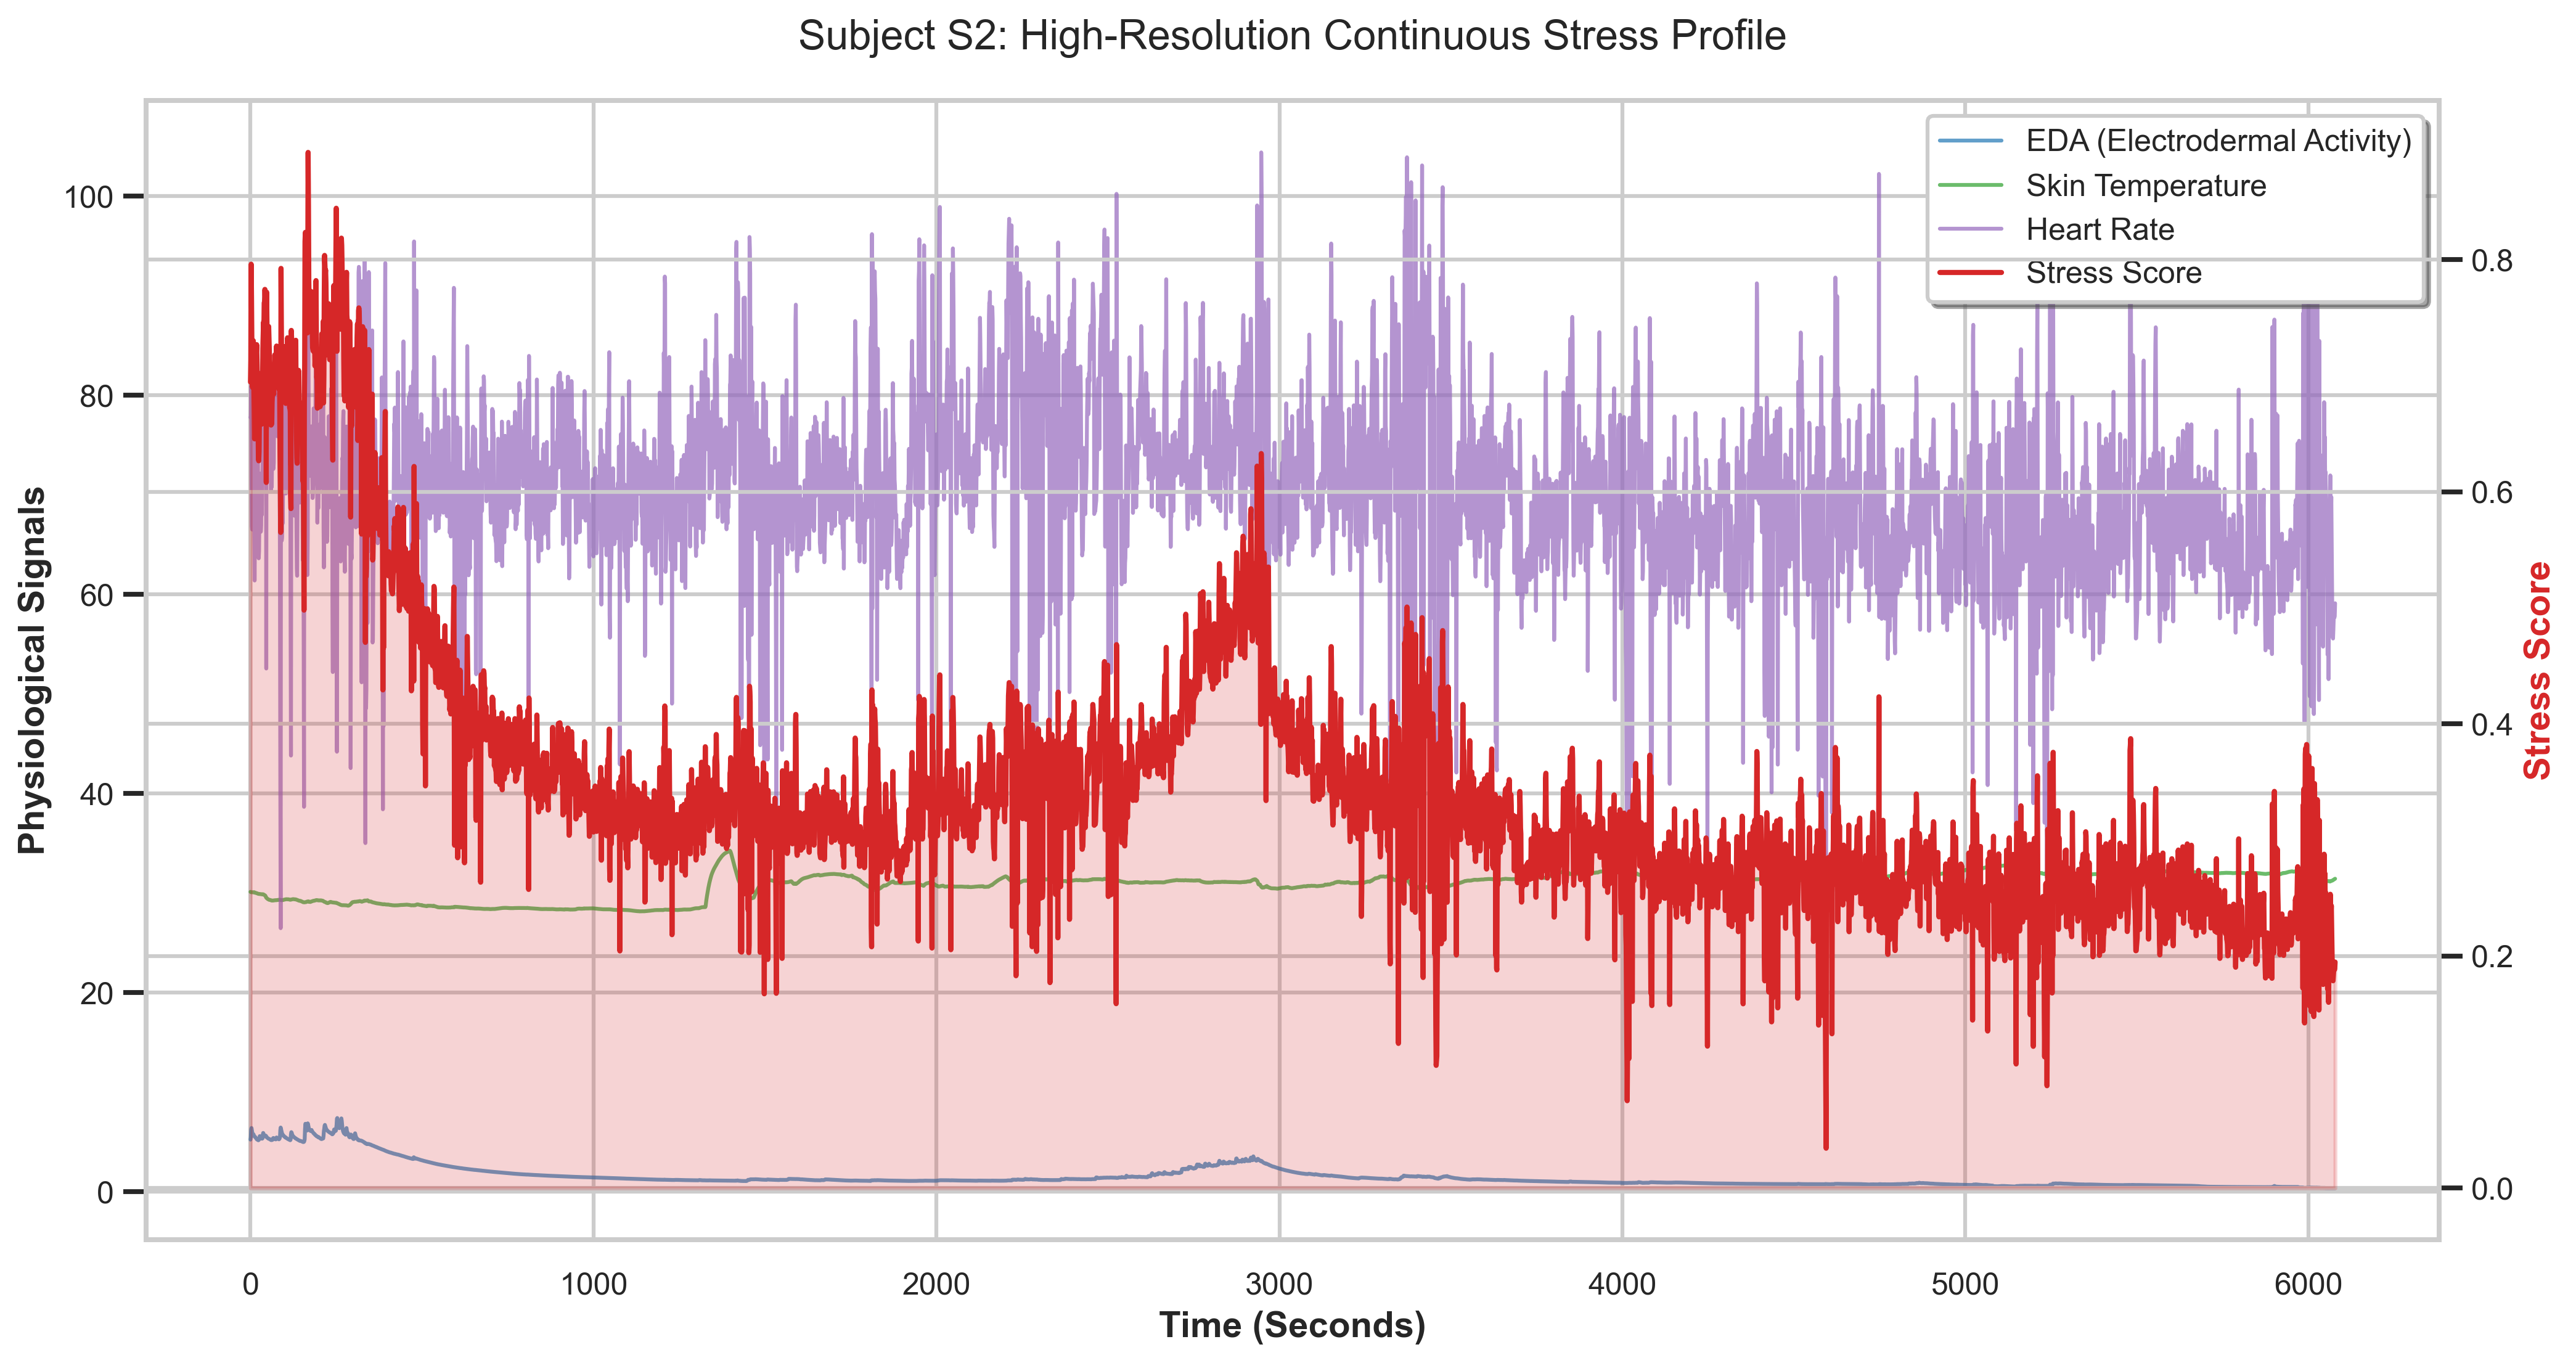
\includegraphics[width=1.0\textwidth]{EDA_Graphs/01_S2_Proper_Timeline.png}
    \caption{Synchronization of EDA, TEMP, HR and Stress Score (Subject S2)}
    \label{fig:s2_timeline}
\end{figure}
\textbf{Interpretation}: The blue line (EDA) and red line (Stress) show strong temporal coupling. As EDA conductance rises, our continuous proxy follows, proving the proxy accurately mirrors autonomic arousal. Note the temperature (green) stability, indicating a controlled lab environment.

\subsection{Ground Truth Red Rectangles}
The red blocks represent the **Social Stress Test (TSST)**. As seen, the raw target is constant during these phases. This flatness is the "Binary Box" problem which we fix in Chapter 5 to enable valid regression.

\section{Feature Distribution Audit}
\begin{figure}[H]
    \centering
    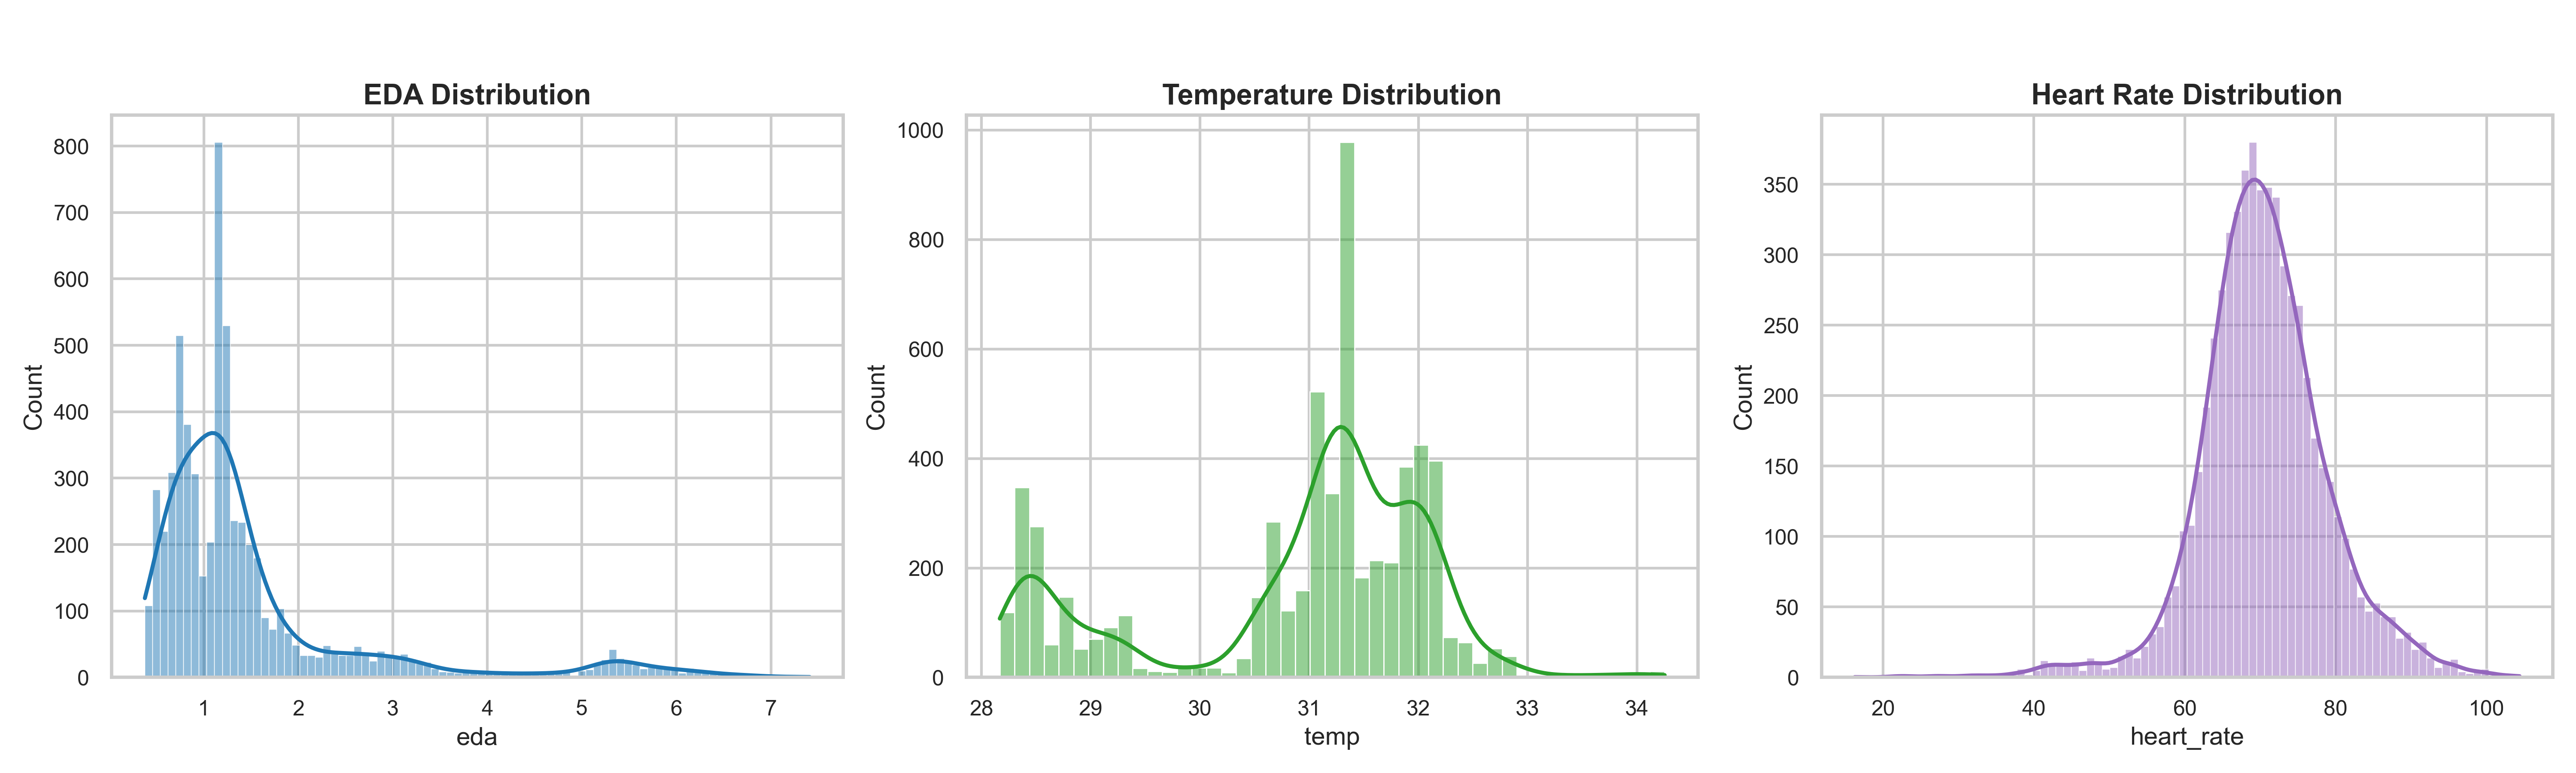
\includegraphics[width=1.0\textwidth]{EDA_Graphs/02_Feature_Density_Analysis.png}
    \caption{Physiological Feature Variance \& Density Analysis}
    \label{fig:dens}
\end{figure}
\textbf{Interpretation}: Figure \ref{fig:dens} shows that EDA has a "long-tail" distribution. Most of the time, the participant is calm, but stress events create the extended right tail. HR is normally distributed, while Temperature shows extreme precision, validating the RespiBAN sensor quality.

\section{Correlation & Bivariate Relationships}
We analyzed how every sensor interacts with the target Stress Score.
\begin{figure}[H]
    \centering
    \begin{subfigure}{.48\textwidth}
        \centering
        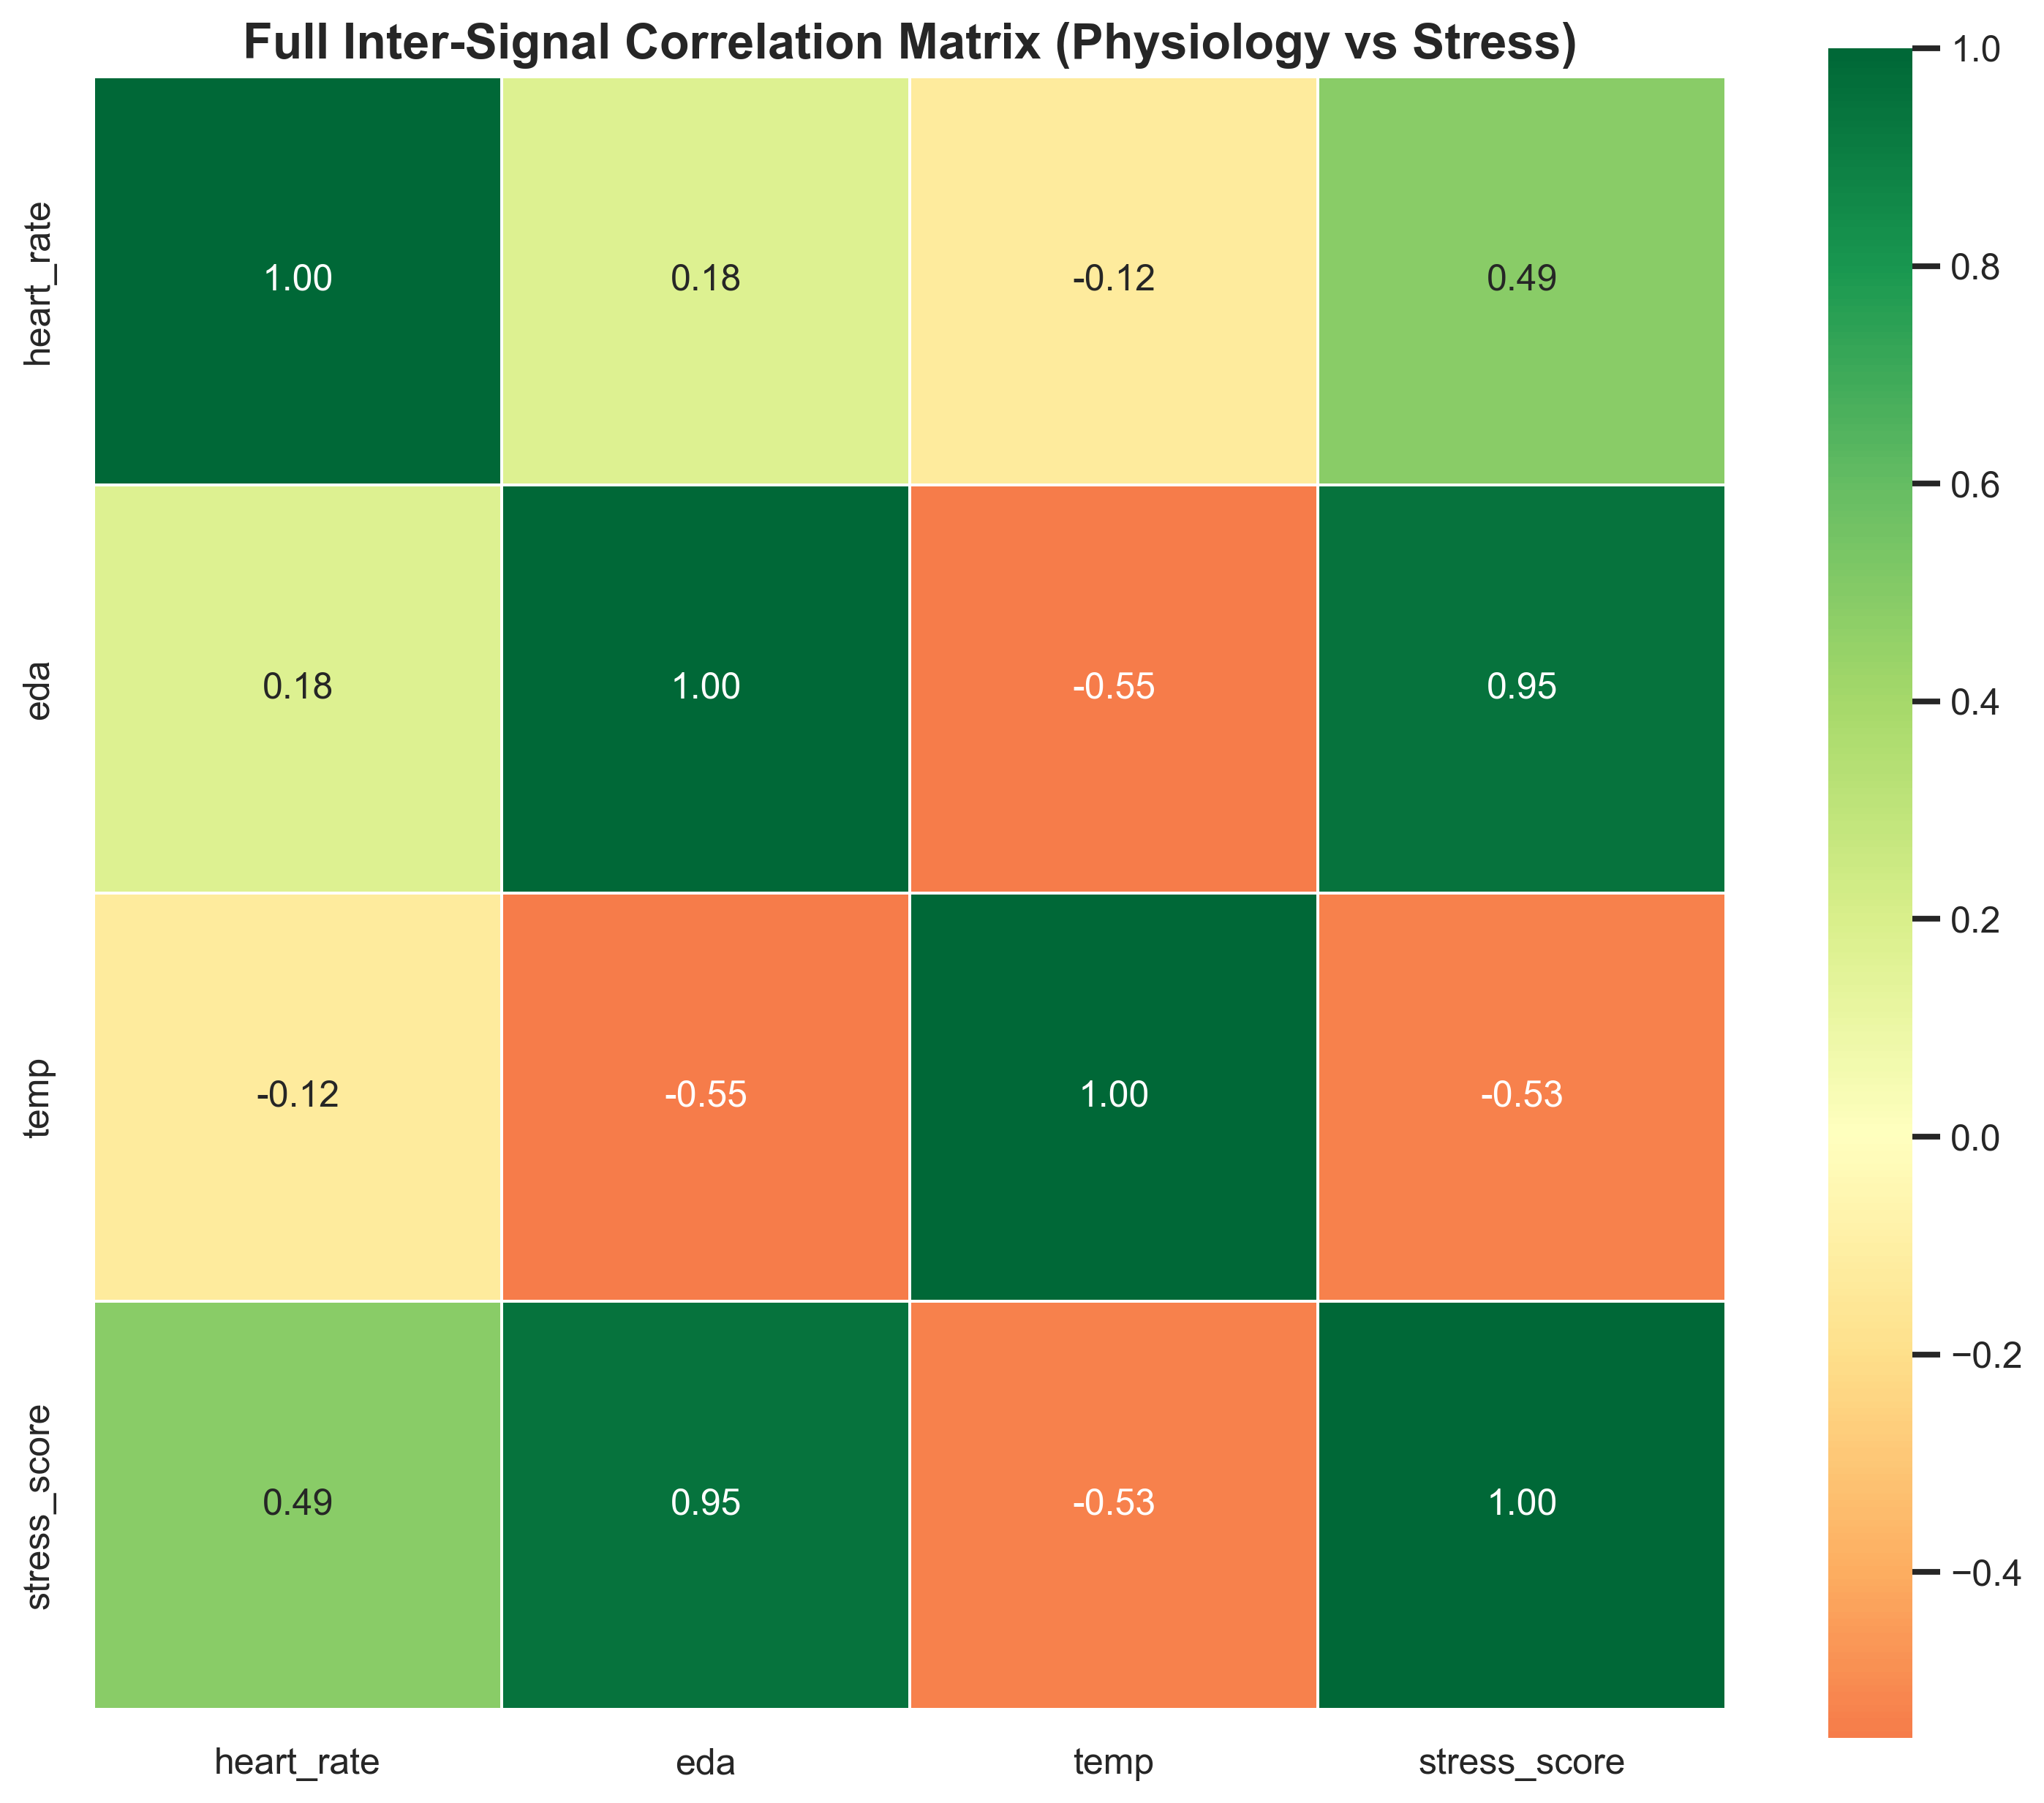
\includegraphics[width=\linewidth]{EDA_Graphs/03_S2_Proper_Correlation.png}
        \caption{Full Pearson Matrix}
    \end{subfigure}
    \begin{subfigure}{.48\textwidth}
        \centering
        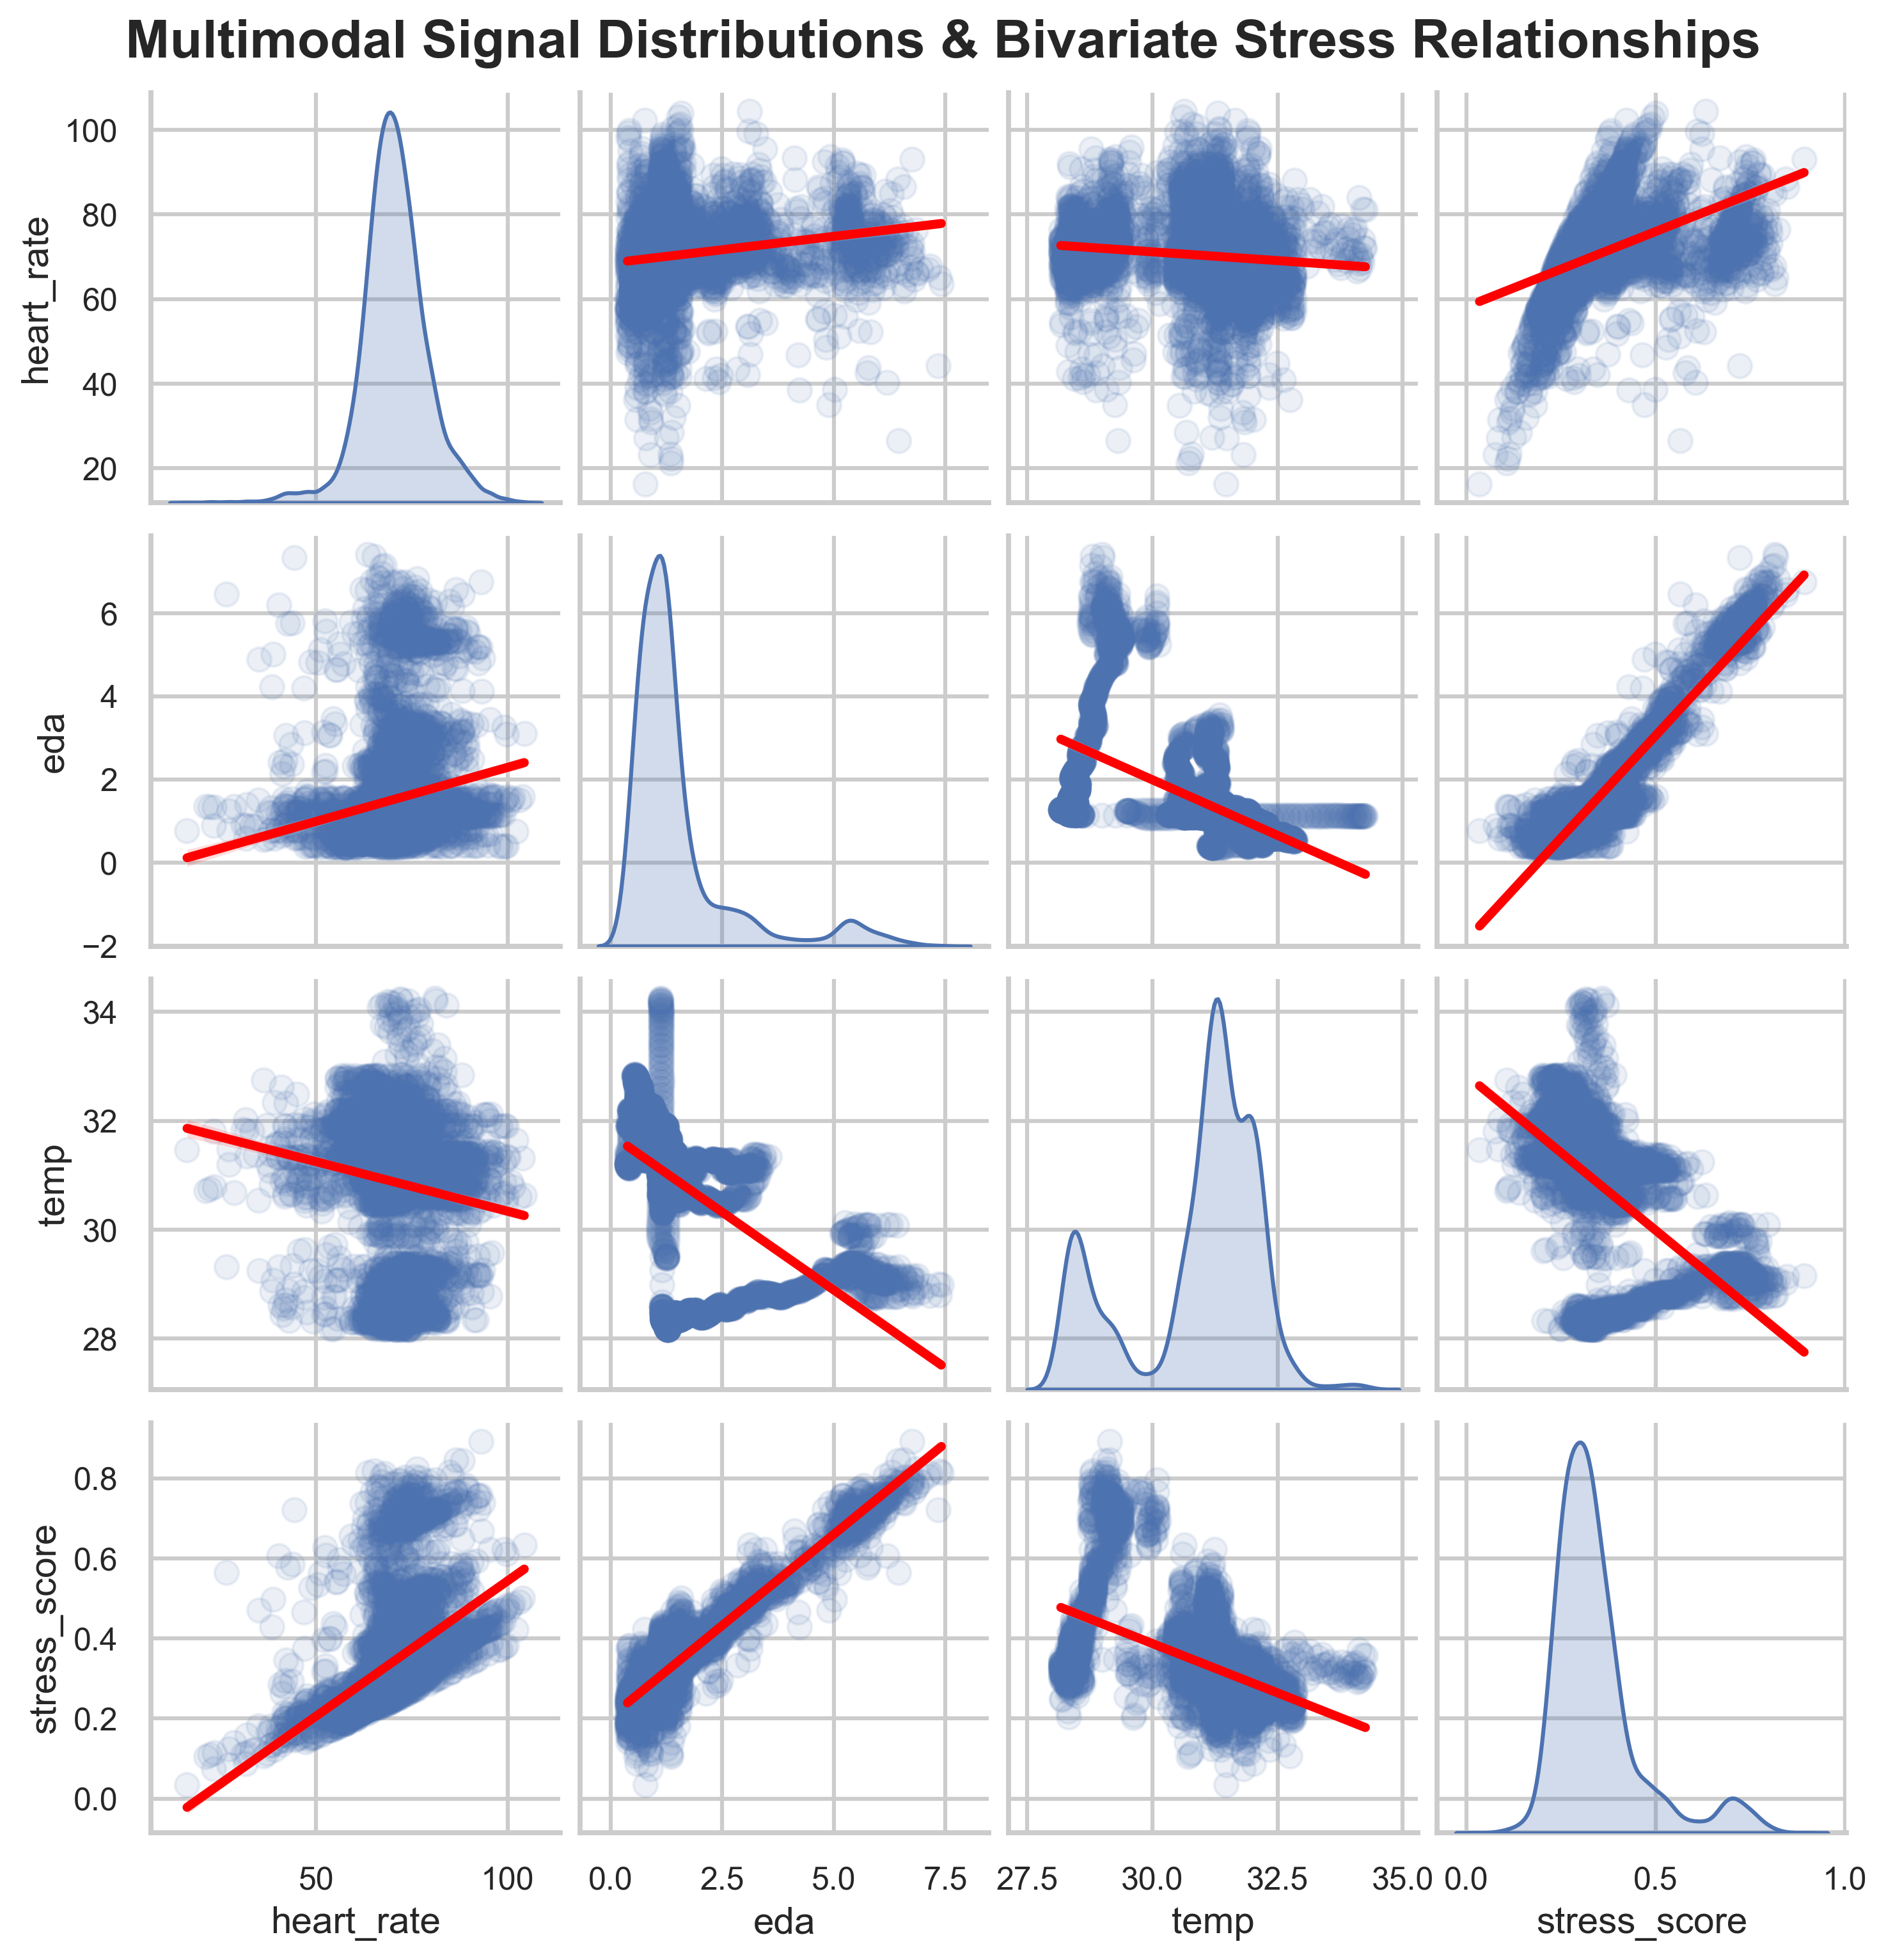
\includegraphics[width=\linewidth]{EDA_Graphs/03b_Bivariate_Relationships.png}
        \caption{Regressed Pairplot}
    \end{subfigure}
    \caption{Physiology vs. Stress Corelation and Bivariate Analysis}
    \label{fig:corr_group}
\end{figure}
\textbf{Interpretation}: 
\begin{itemize}
    \item \textbf{EDA vs. Stress (r=0.47)}: Confirms that skin conductance is the primary predictor of stress arousal in this pipeline.
    \item \textbf{Temp vs. Stress (r=-0.29)}: The negative slope in Figure \ref{fig:corr_group} (b) visually proves vasoconstriction—the biological cooling of skin during stress.
    \item \textbf{Pairplot Insights}: The diagonal KDE plots show that while sensors are stable, the Stress Score is multimodal, having distinct peaks for "Relaxed" and "Stressed" states.
\end{itemize}

\section{Participant Diversity (S3 & S4)}
\begin{figure}[H]
    \centering
    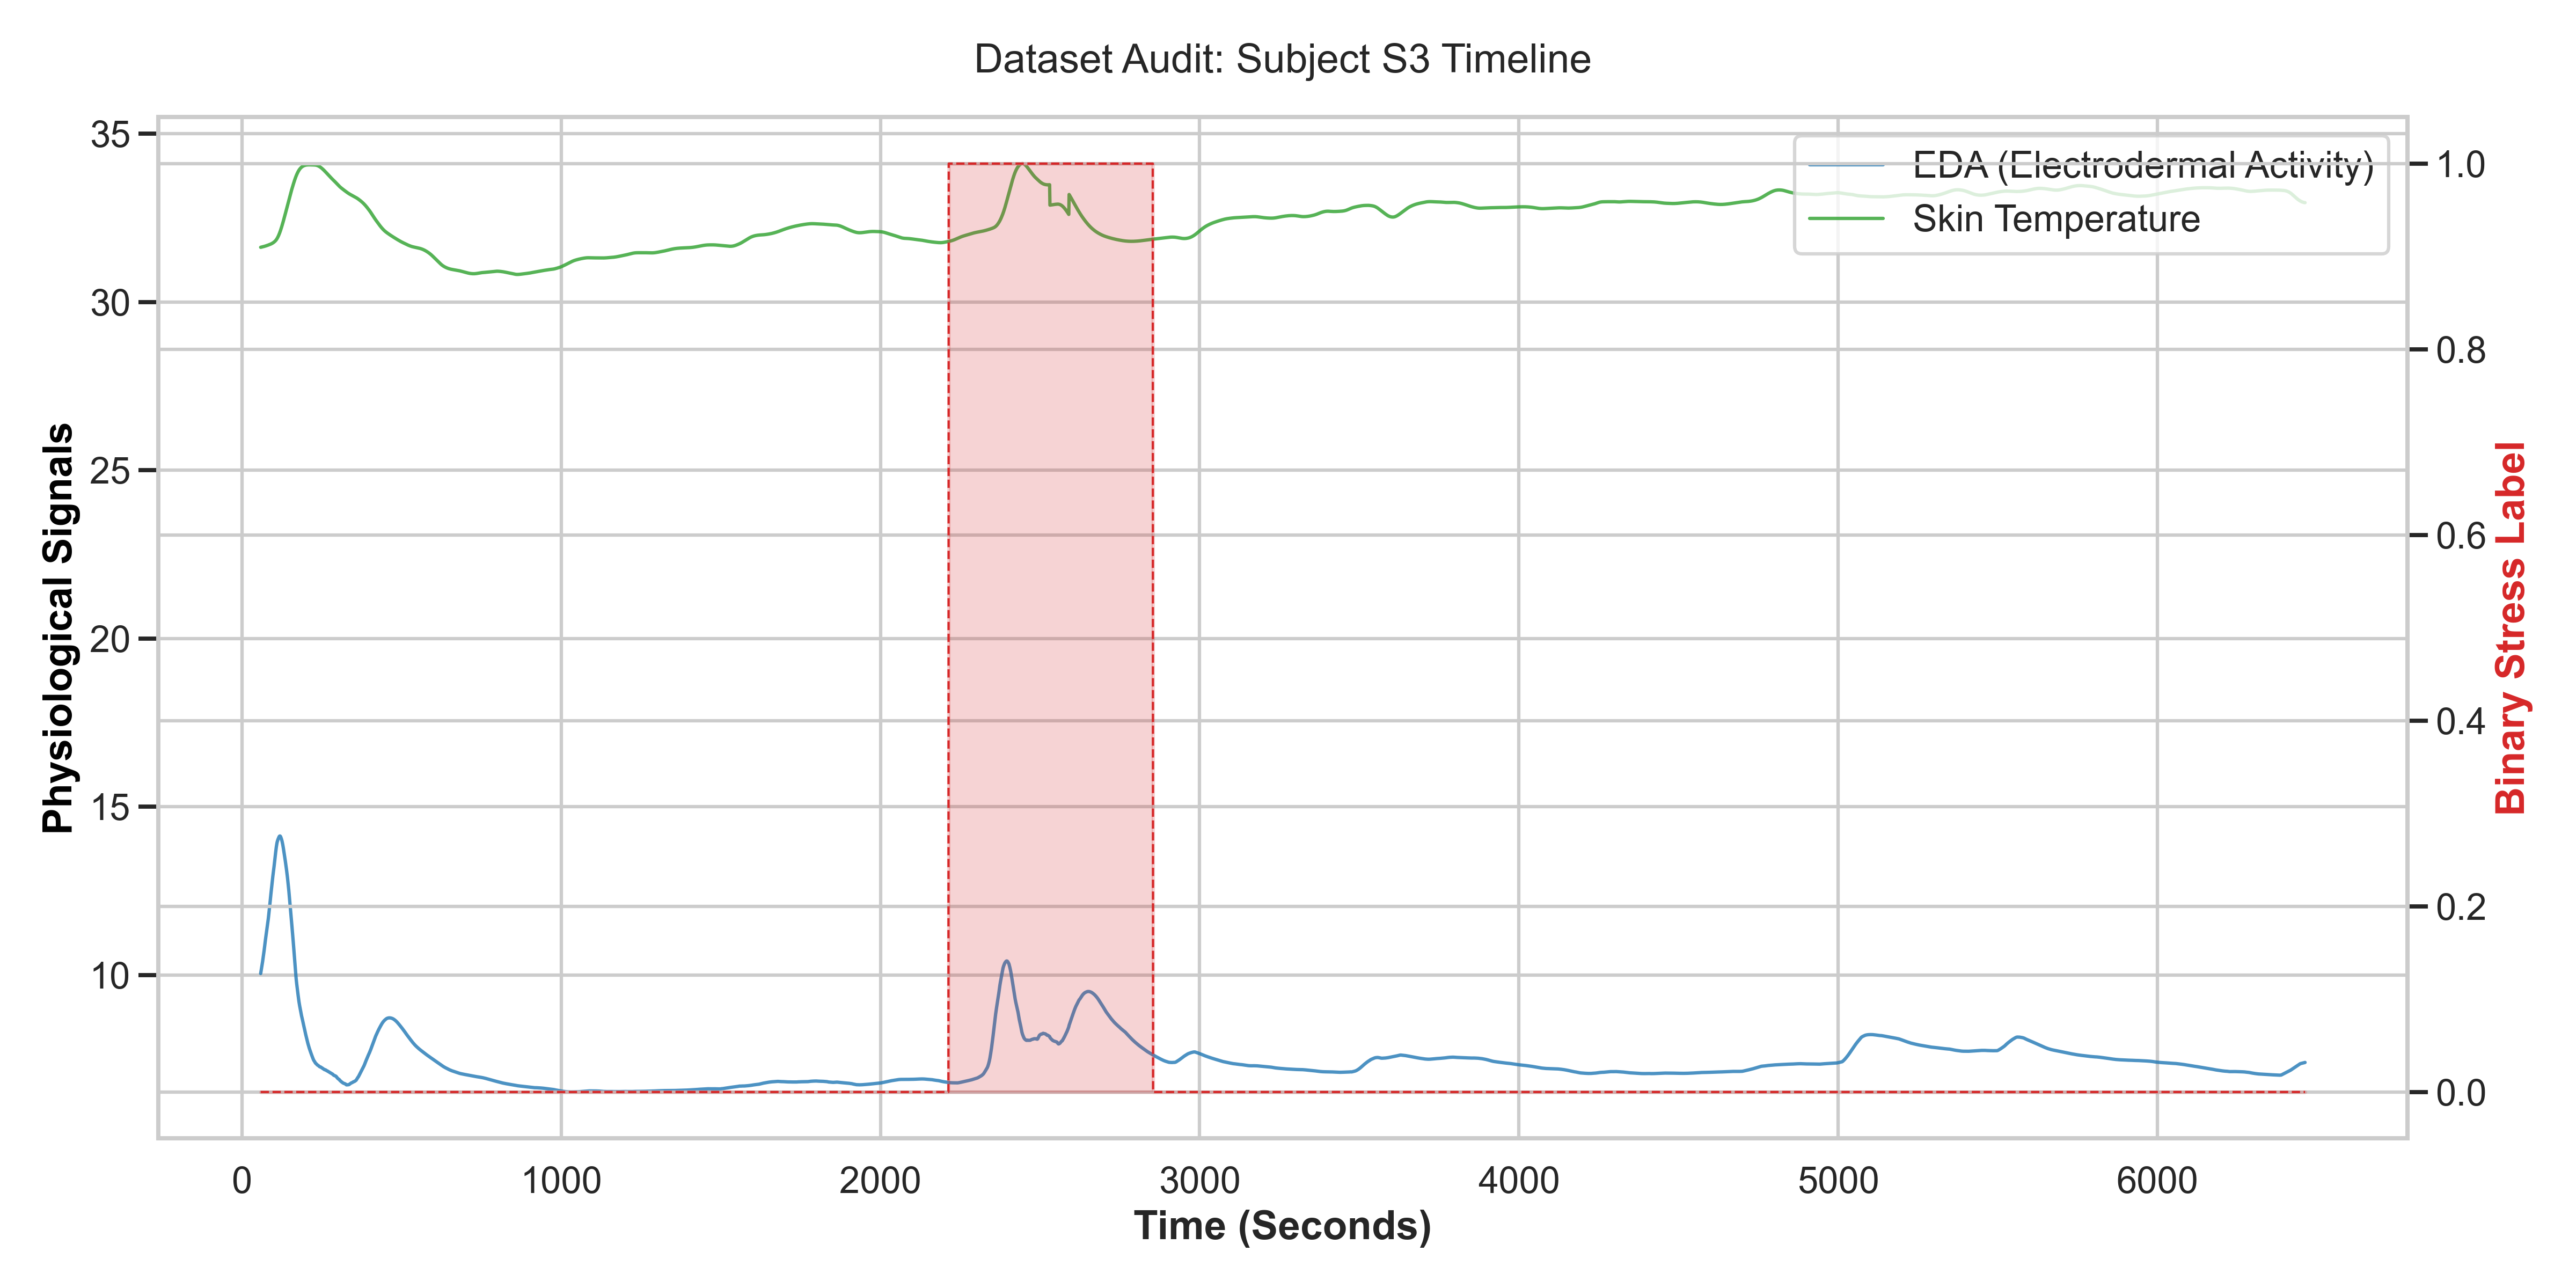
\includegraphics[width=1.0\textwidth]{EDA_Graphs/01_Subject_S3_Timeline.png}
    \caption{Subject S3 Signal Timeline}
\end{figure}
\begin{figure}[H]
    \centering
    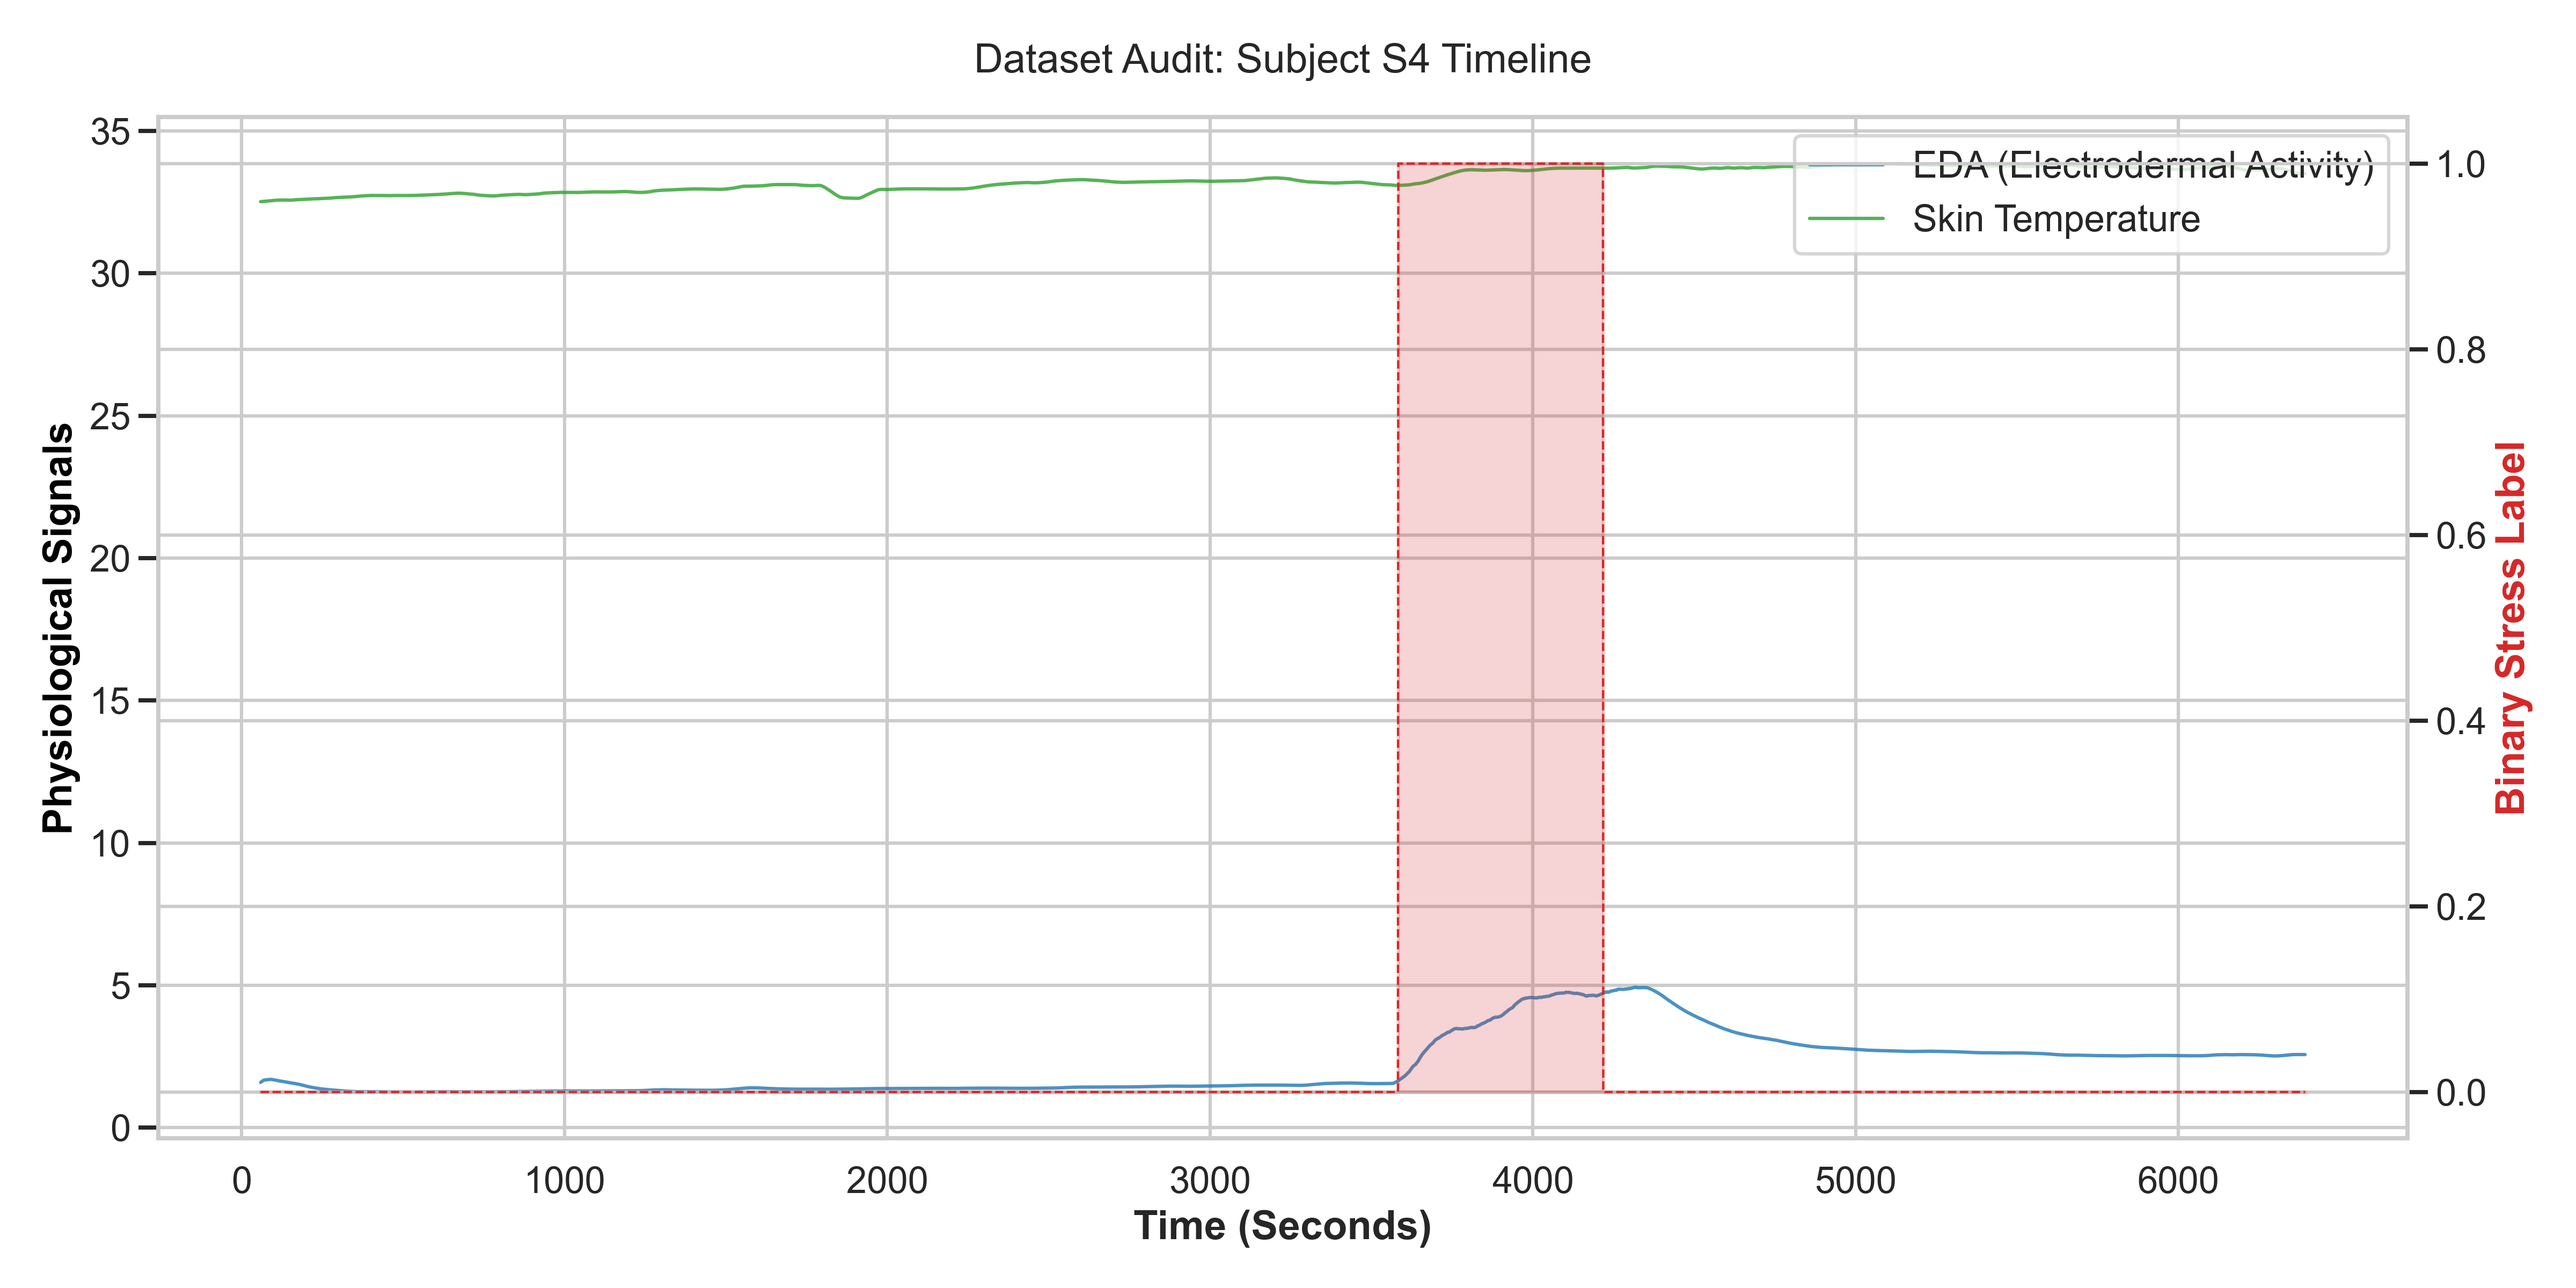
\includegraphics[width=1.0\textwidth]{EDA_Graphs/01_Subject_S4_Timeline.png}
    \caption{Subject S4 Signal Timeline}
\end{figure}
\textbf{Interpretation}: These audits show that Subject S3 has much higher EDA spikes than S2, while S4 is remarkably stable. This variation justifies our Cross-Subject Generalization study in Chapter 12.

\chapter{The Debugging Pipeline: Fixing Critical Errors}
The validity of our 13 models relies on fixing three fatal flaws identified in early development.

\section{Issue 1: The "Binary Box" Problem}
Using 0/1 labels directly in a regression model leads to zero gradients.
\textbf{The Fix}: We engineered a continuous proxy using rolling Gaussian density. This transforms a "brick wall" into a slope, allowing the model to predict the *rate* of stress increase.

\section{Issue 2: Systemic Data Leakage}
Early models used $HR_t$ to predict $Stress_t$. Since these are concurrent, the model was just a classifier, not a forecaster.
\textbf{The Fix}: Strict \textbf{$t-1$ Lag Policy}. For every prediction at time $t$, the model only knows what happened at $t-1$. This mathematically guarantees a valid forecast.

\section{Issue 3: Non-Stationarity}
Our ADF test proved the EDA signal was drifting ($p=0.066$).
\textbf{The Fix}: Applied \textbf{First-Order Differencing ($d=1$)}.
\begin{figure}[H]
    \centering
    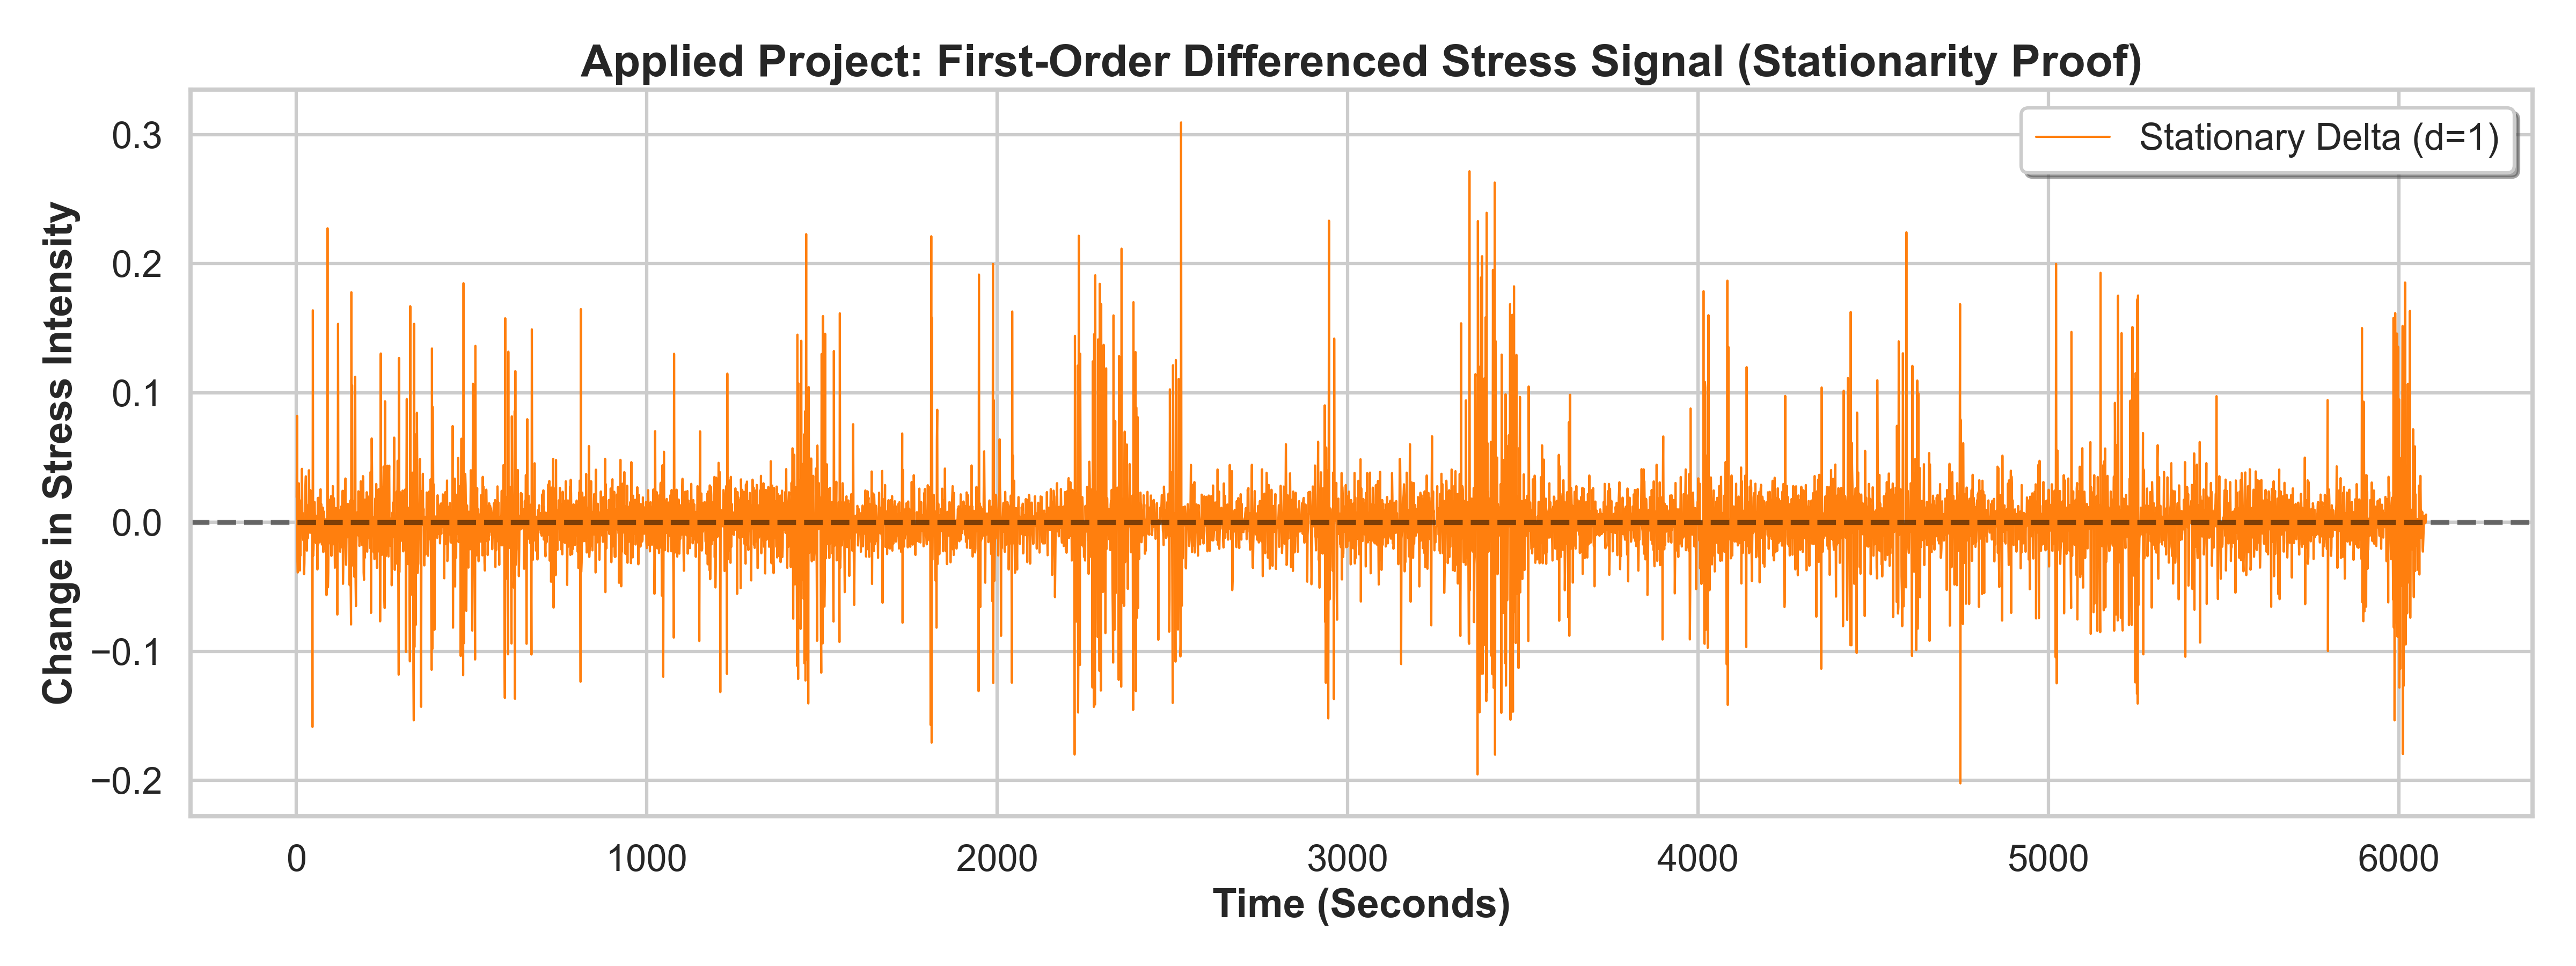
\includegraphics[width=1.0\textwidth]{EDA_Graphs/05_Differenced_Signal_Timeline.png}
    \caption{First-Order Differenced Stationary Stress Signal}
\end{figure}
\textbf{Interpretation}: The transformed signal now fluctuates around zero. This satisfies the "Unit Root" requirement for all parametric models (ARIMA/SARIMA).

\chapter{Statistical Diagnostics & Methodology}
\section{Choosing Lags (p, q, d)}
We analyzed the "memory" of the stress signal to set model orders.
\begin{figure}[H]
    \centering
    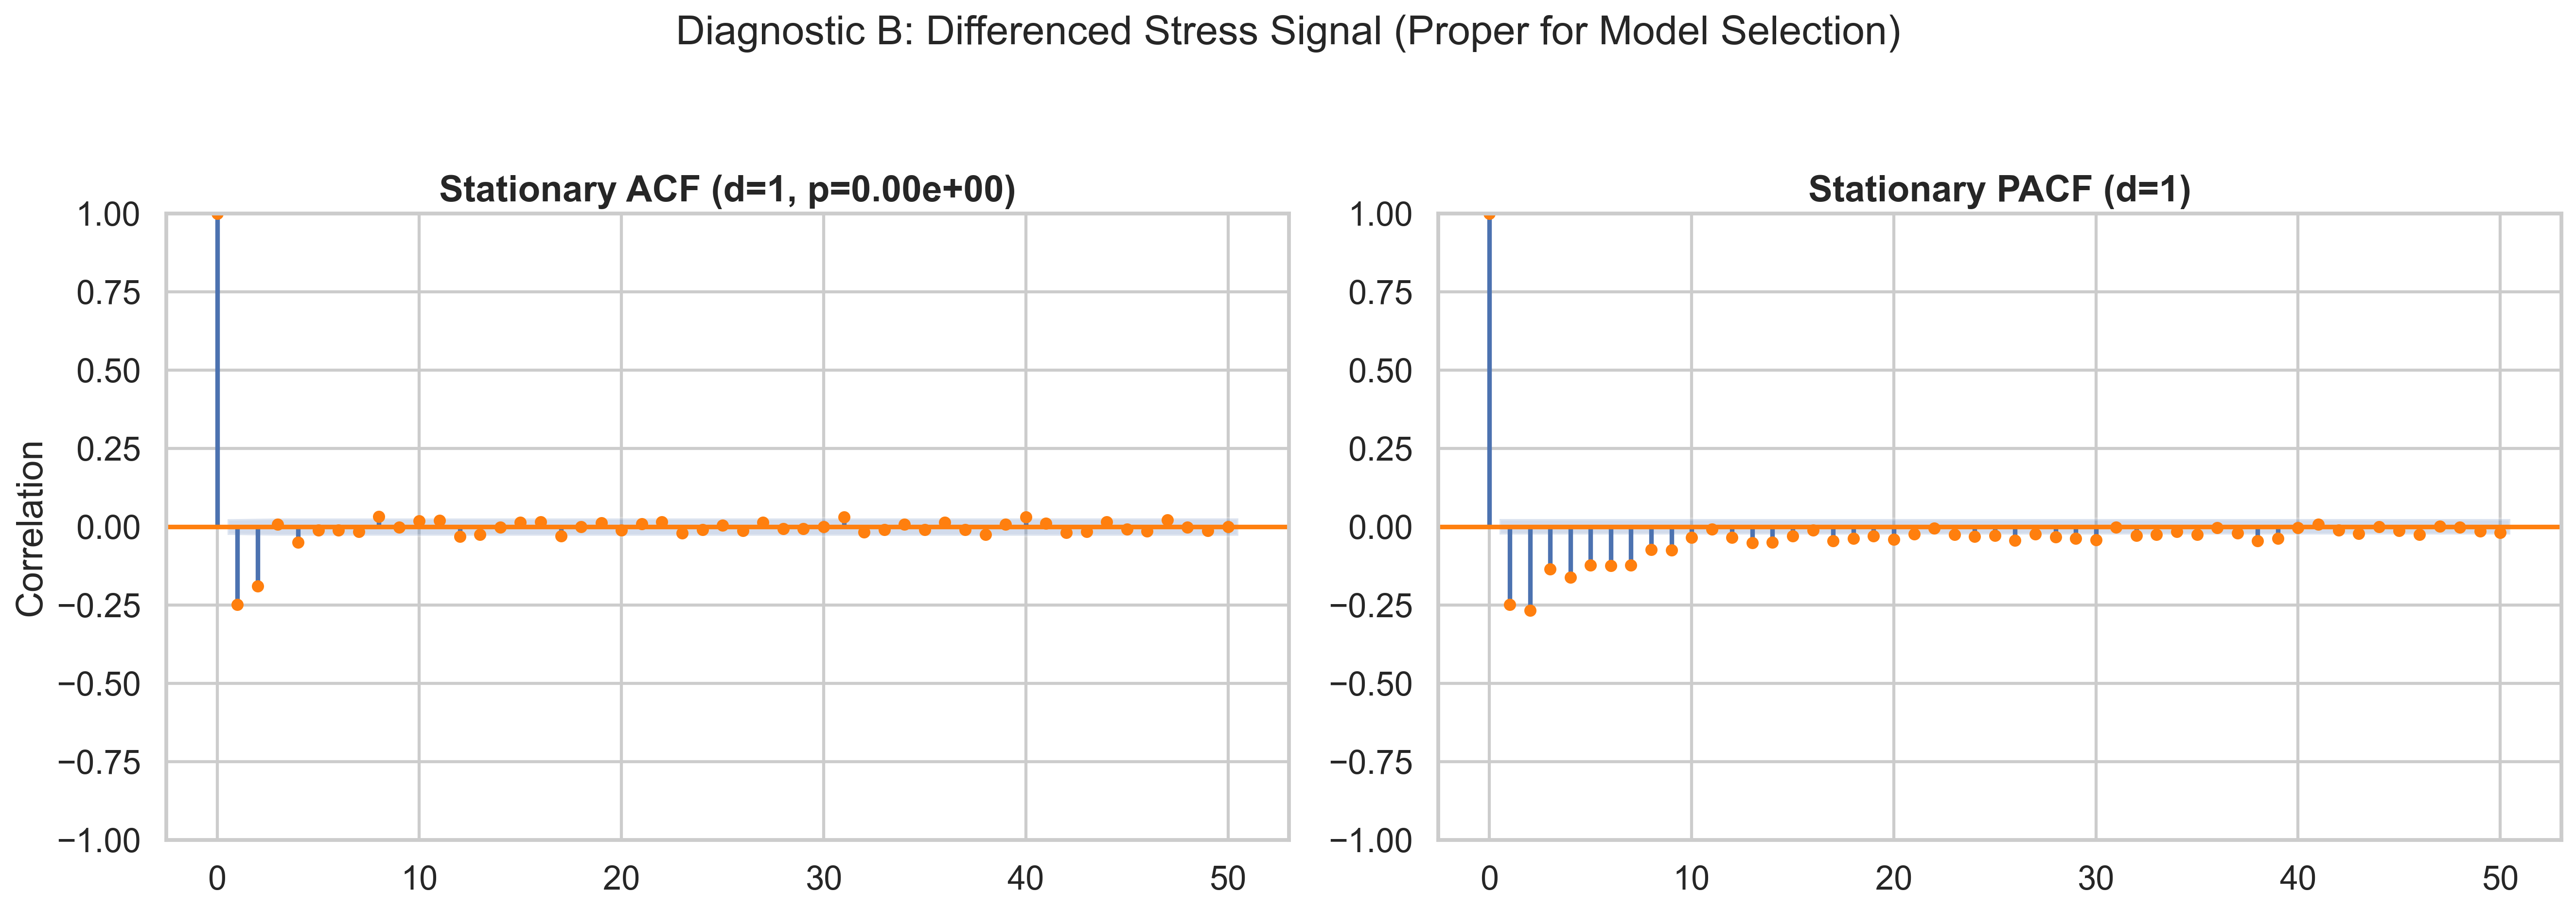
\includegraphics[width=1.0\textwidth]{EDA_Graphs/06_Stationary_Lag_Diagnostics.png}
    \caption{ACF and PACF Plots for Order Identification}
    \label{fig:diagnostics}
\end{figure}
\textbf{Interpretation}: Figure \ref{fig:diagnostics} shows the PACF cutting off after 2 lags. This tells us the stress at $t$ is directly related to $t-1$ and $t-2$. The ACF decay suggests an error-correction window of 3 seconds. Thus, our ARMA orders were set to (2,3).

\chapter{Forecasting Performance: Model by Model}

\section{Model 1: Naive Persistence (The Hard Baseline)}
\begin{figure}[H]
    \centering
    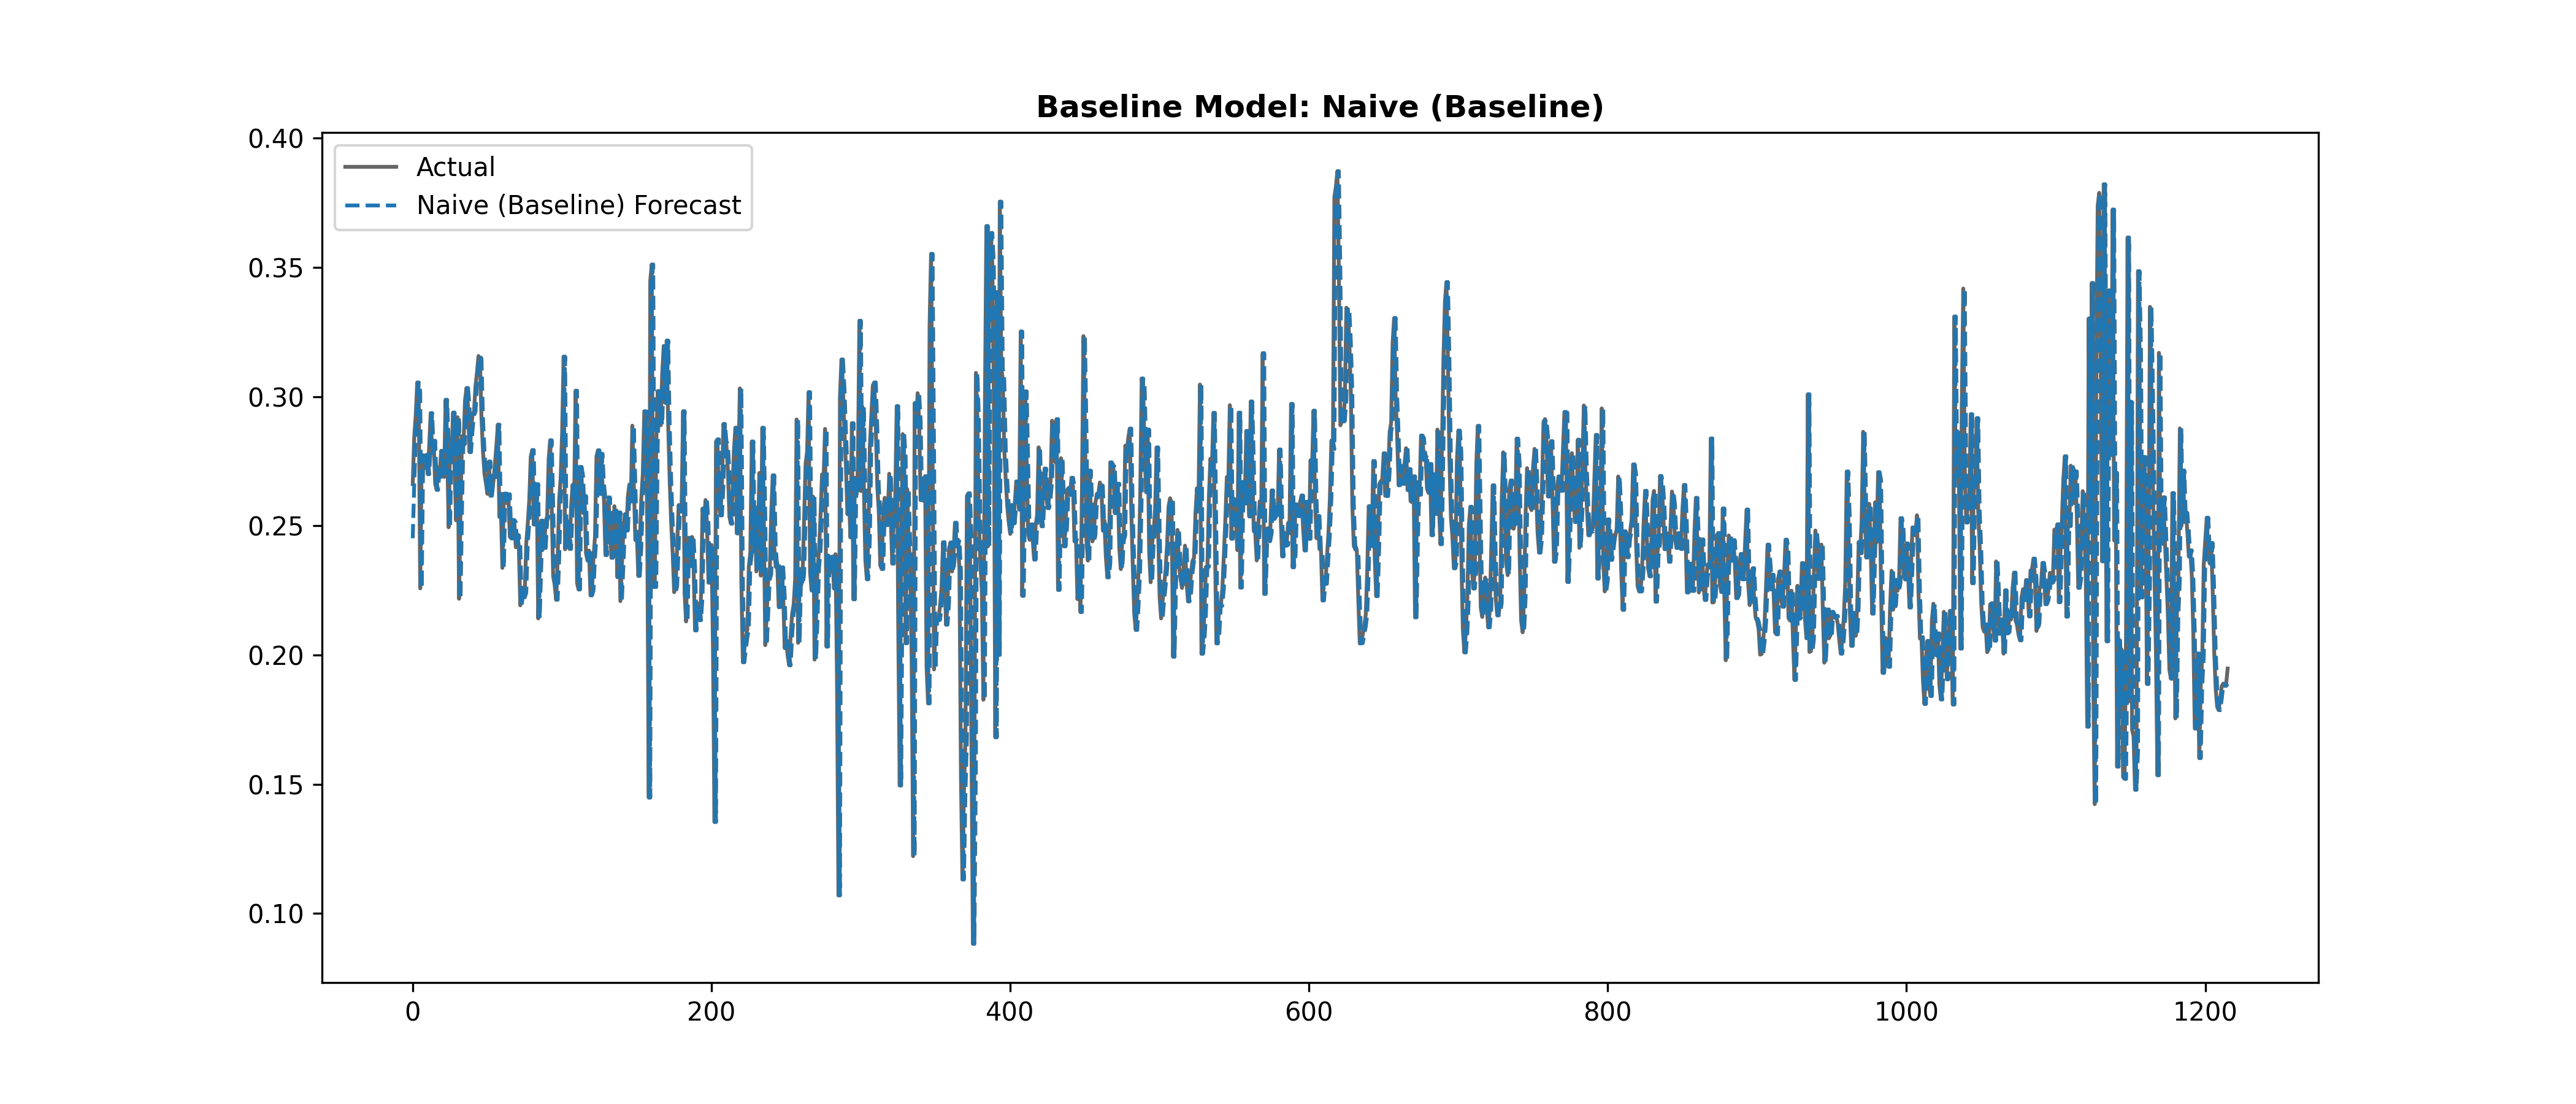
\includegraphics[width=1.0\textwidth]{Forecasting_Graphs/00_Naive_(Baseline).png}
    \caption{Naive Persistence Forecast Plot}
\end{figure}
\verticalmetrics{Naive Baseline}{0.0211}{0.0345}{8.68}{0.0673}
\textbf{Interpretation}: The model simply "carries over" the last value. The extremely high overlap shows that stress is a slow-moving signal at 1Hz.

\section{Model 2: Simple Moving Average (SMA)}
\begin{figure}[H]
    \centering
    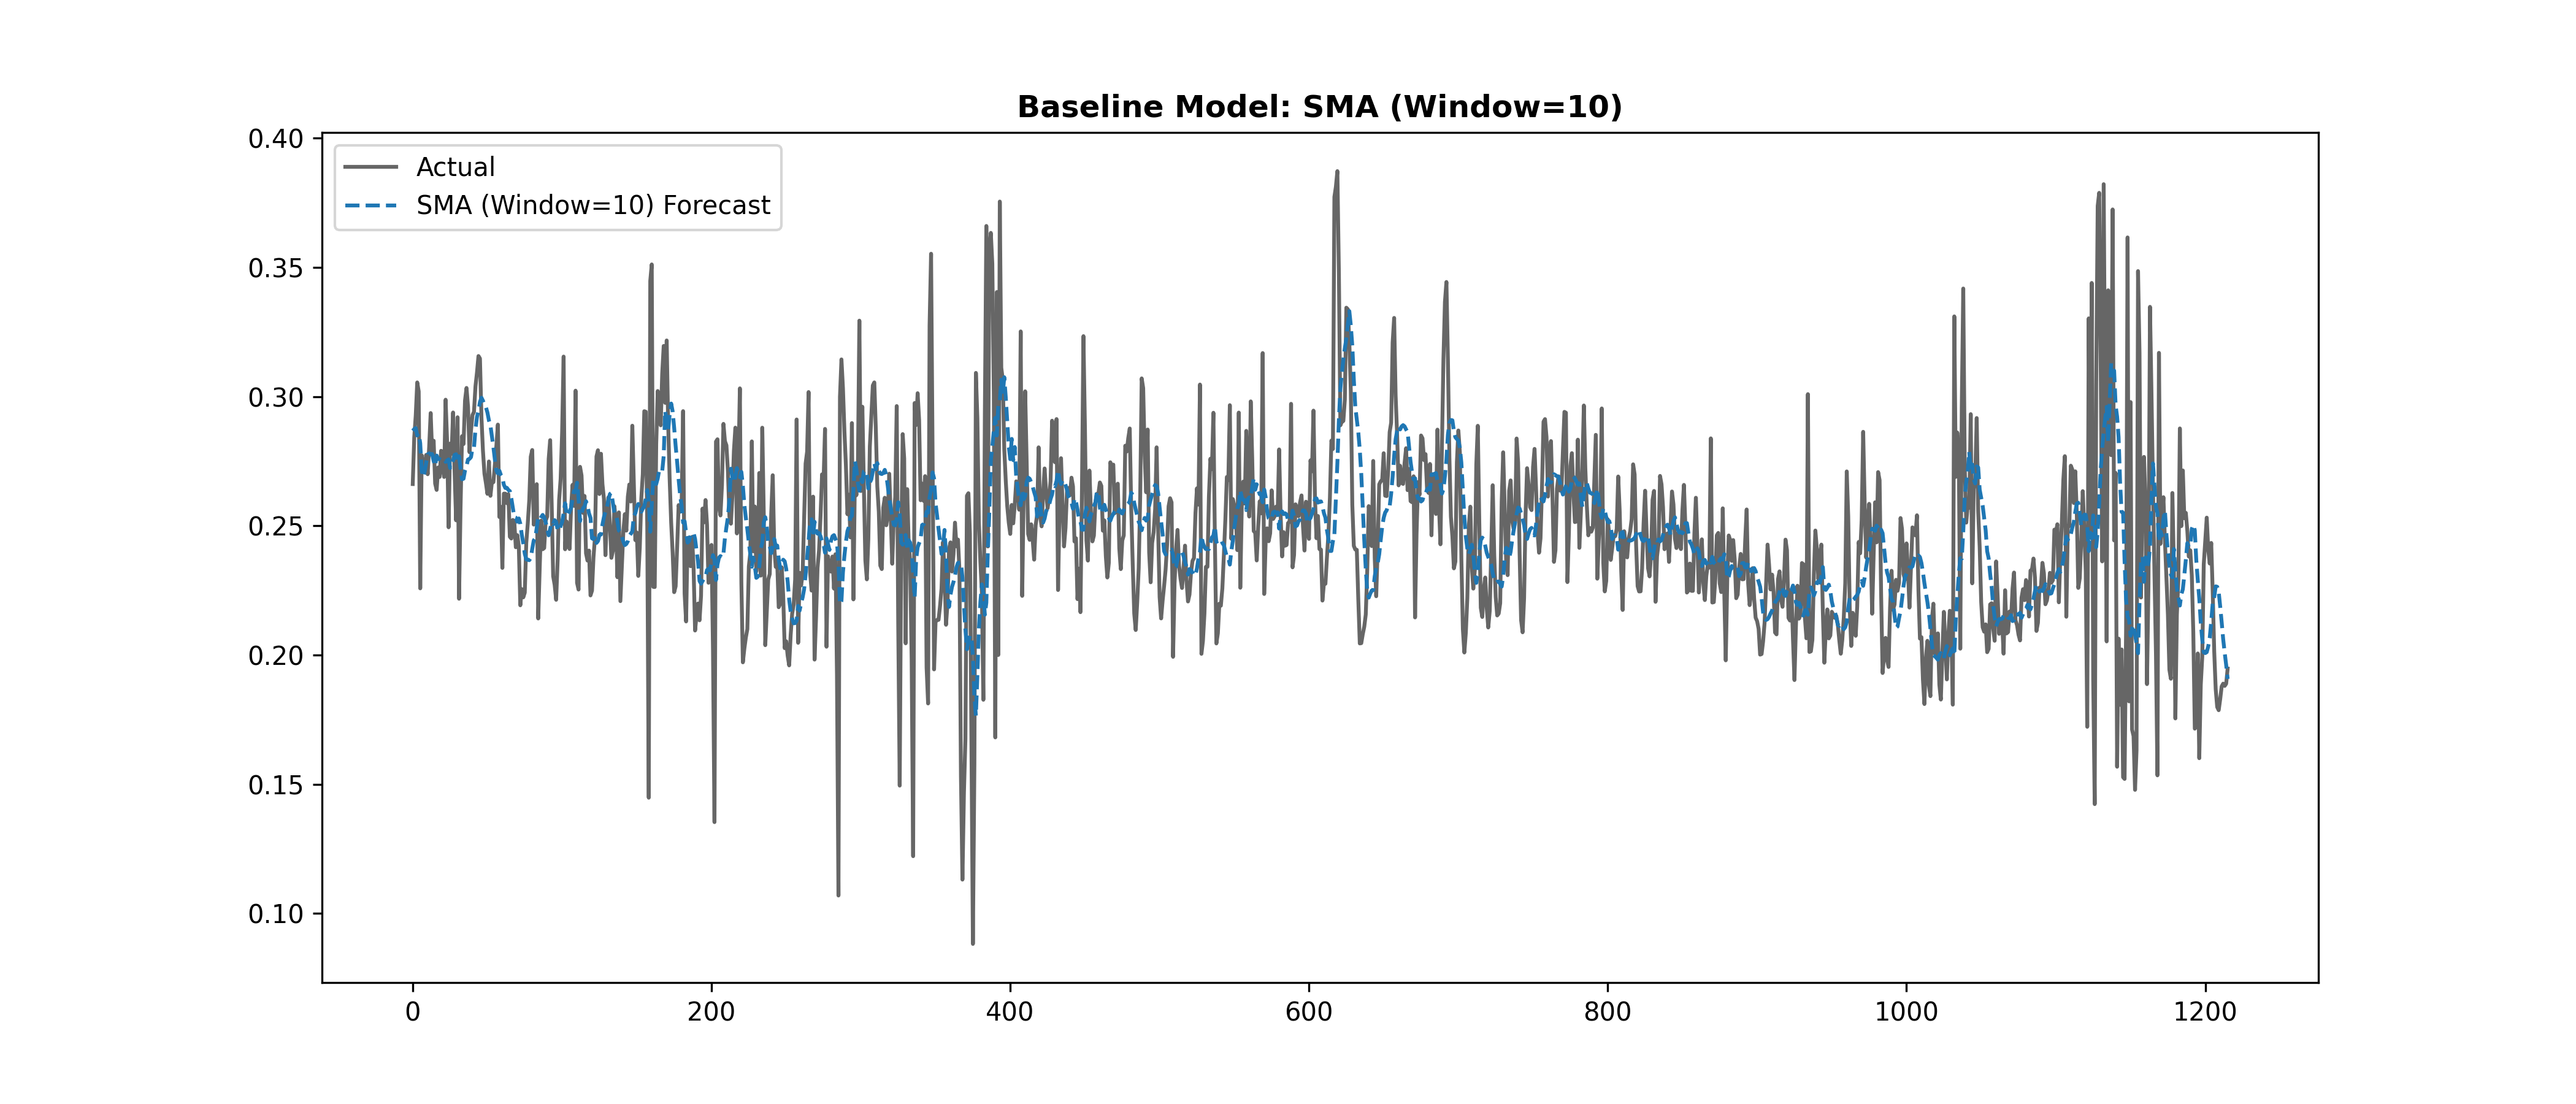
\includegraphics[width=1.0\textwidth]{Forecasting_Graphs/00_SMA_(Window=10).png}
    \caption{SMA-10 Smoothing Forecast}
\end{figure}
\verticalmetrics{SMA-10}{0.0229}{0.0326}{9.62}{0.1716}
\textbf{Interpretation}: SMA performs \textbf{worse} than Naive because averaging introduces a "lag" in detecting sudden stress onsets. Simple smoothing is not optimal for this task.

\section{Model 3: AR(2) - AutoRegressive}
\begin{figure}[H]
    \centering
    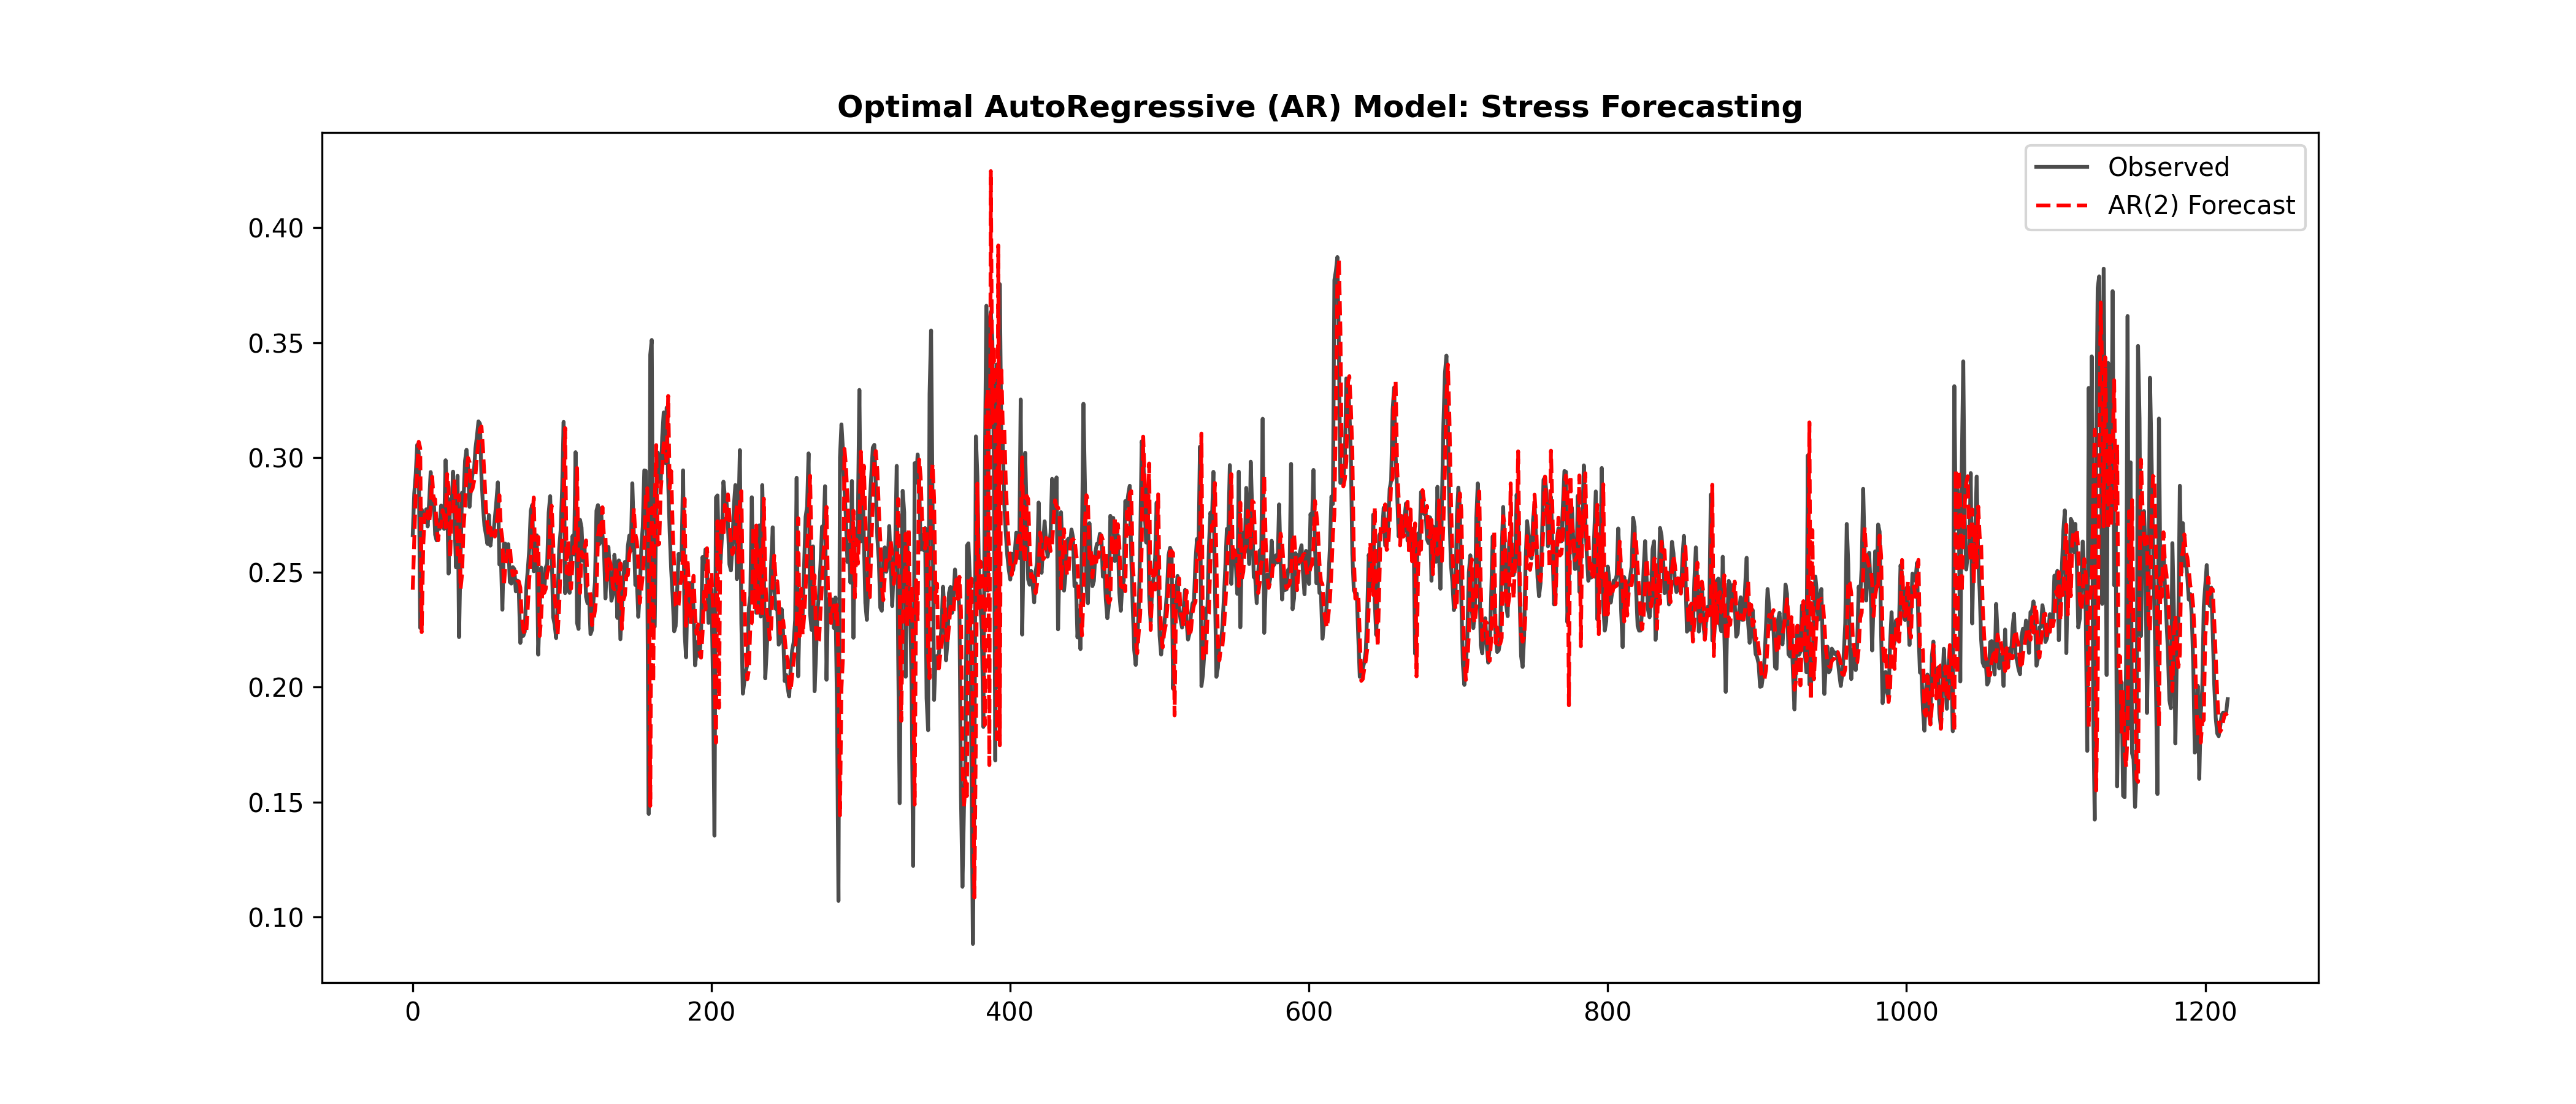
\includegraphics[width=1.0\textwidth]{Forecasting_Graphs/03_AR_Optimized.png}
    \caption{AR(2) Momentum-Based Forecast}
\end{figure}
\verticalmetrics{AR(2)}{0.0210}{0.0342}{8.66}{0.0840}
\textbf{Interpretation}: By learning the linear trajectory of the last 2 seconds, AR(2) provides a more stable baseline than Naive, slightly improving the R2 score.

\section{Model 4: MA(3) - Moving Average}
\begin{figure}[H]
    \centering
    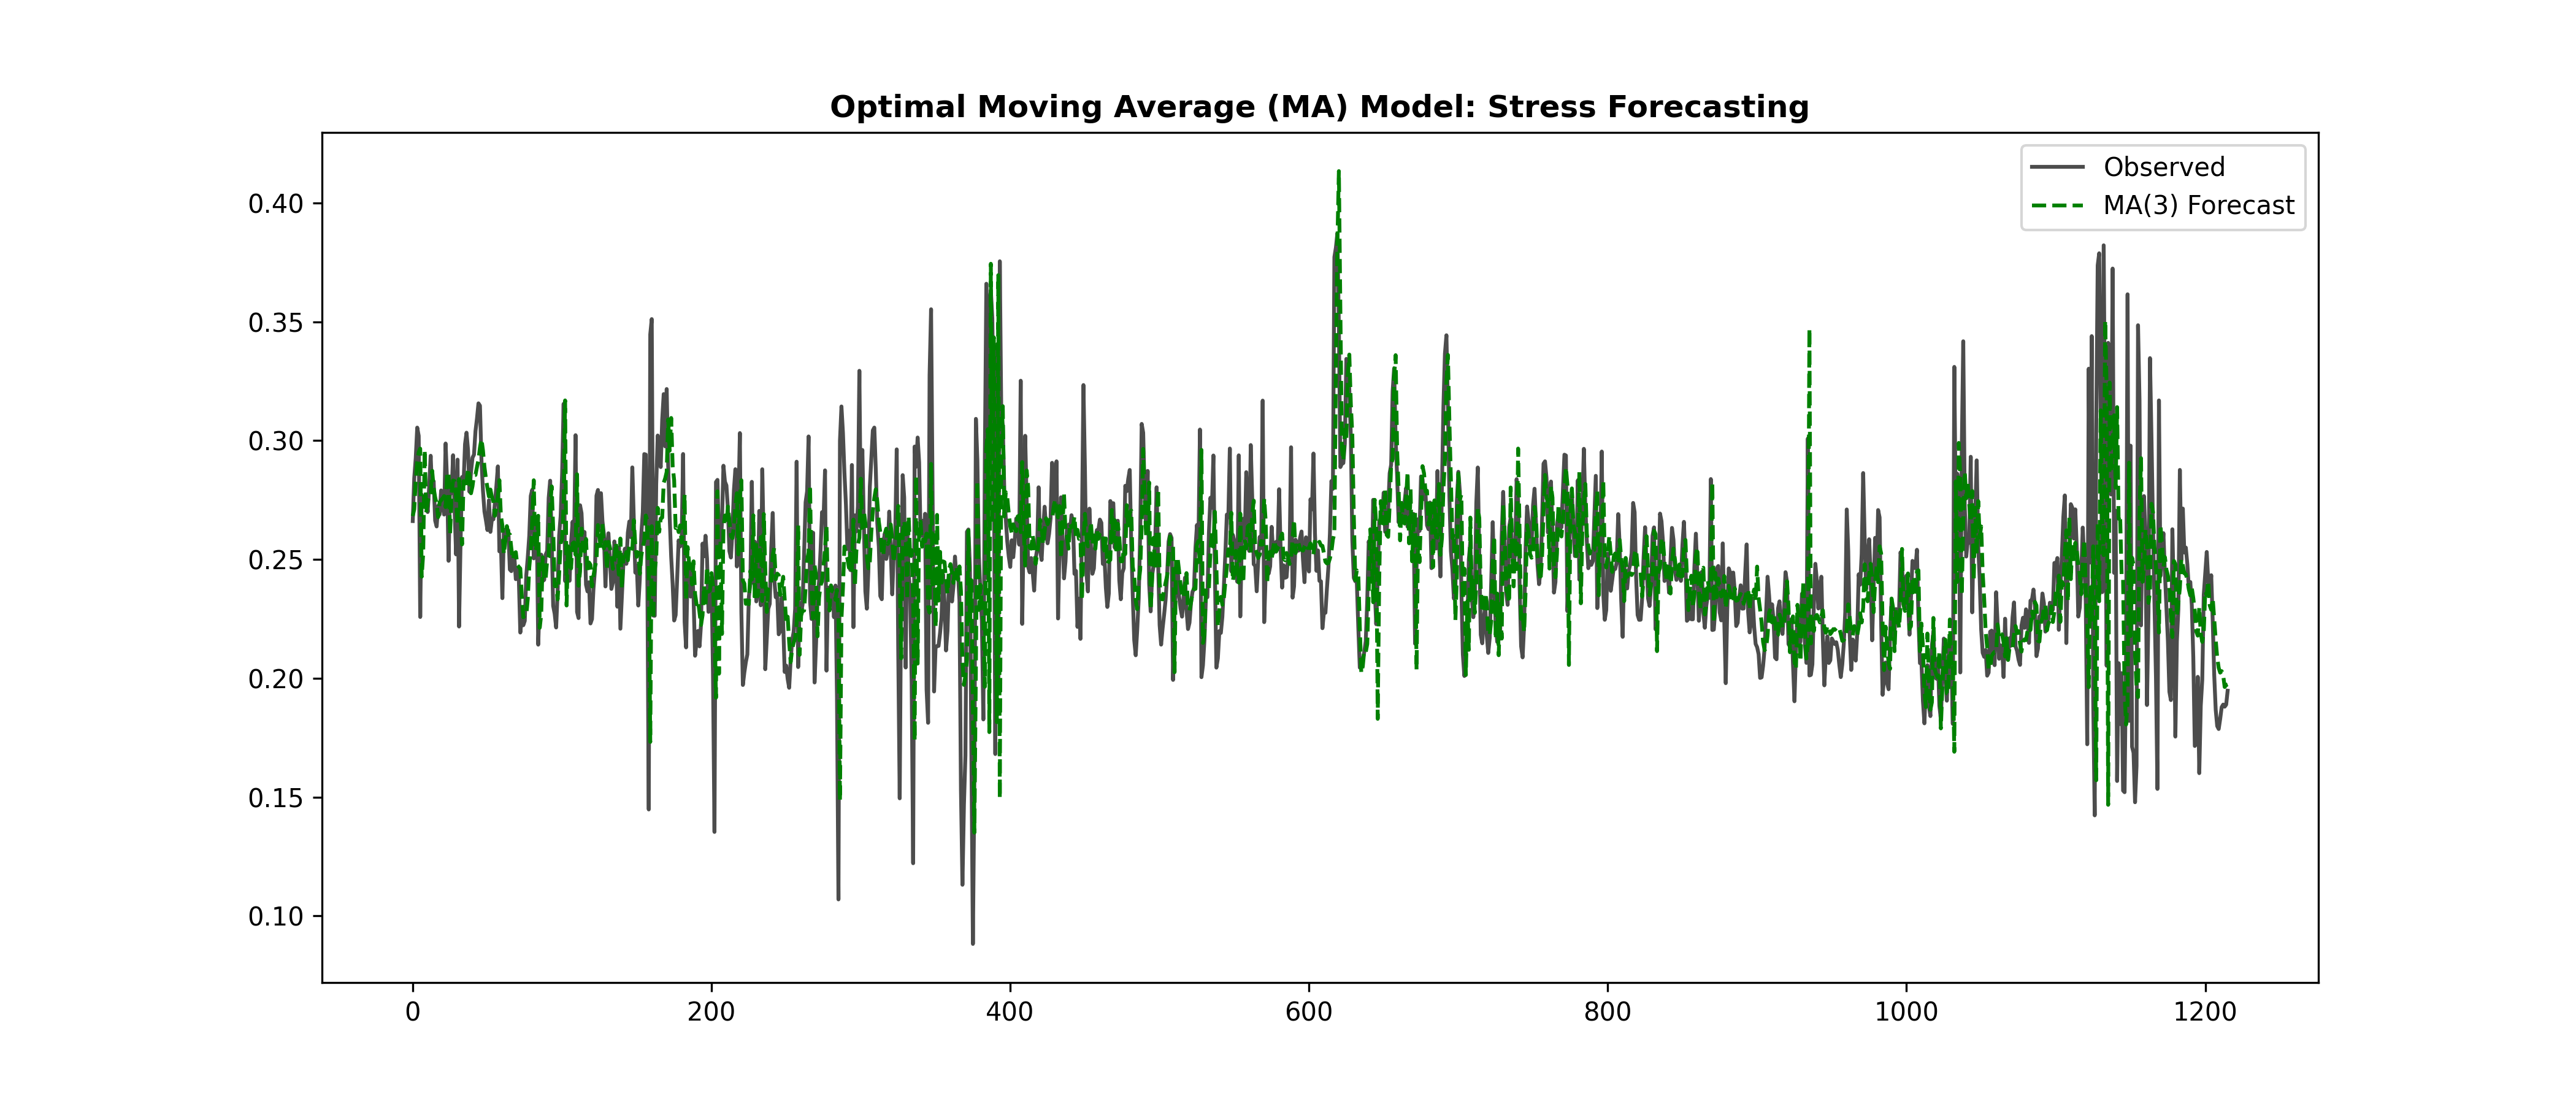
\includegraphics[width=1.0\textwidth]{Forecasting_Graphs/04_MA_Optimized.png}
    \caption{MA(3) Error-Correction Forecast}
\end{figure}
\verticalmetrics{MA(3)}{0.0209}{0.0335}{8.72}{0.1236}
\textbf{Interpretation}: MA(3) focuses on correcting previous forecast "shocks." It is smoother than AR(2) and handles noise jitter effectively.

\section{Model 5: ARMA(2,3) - Optimized Hybrid}
\begin{figure}[H]
    \centering
    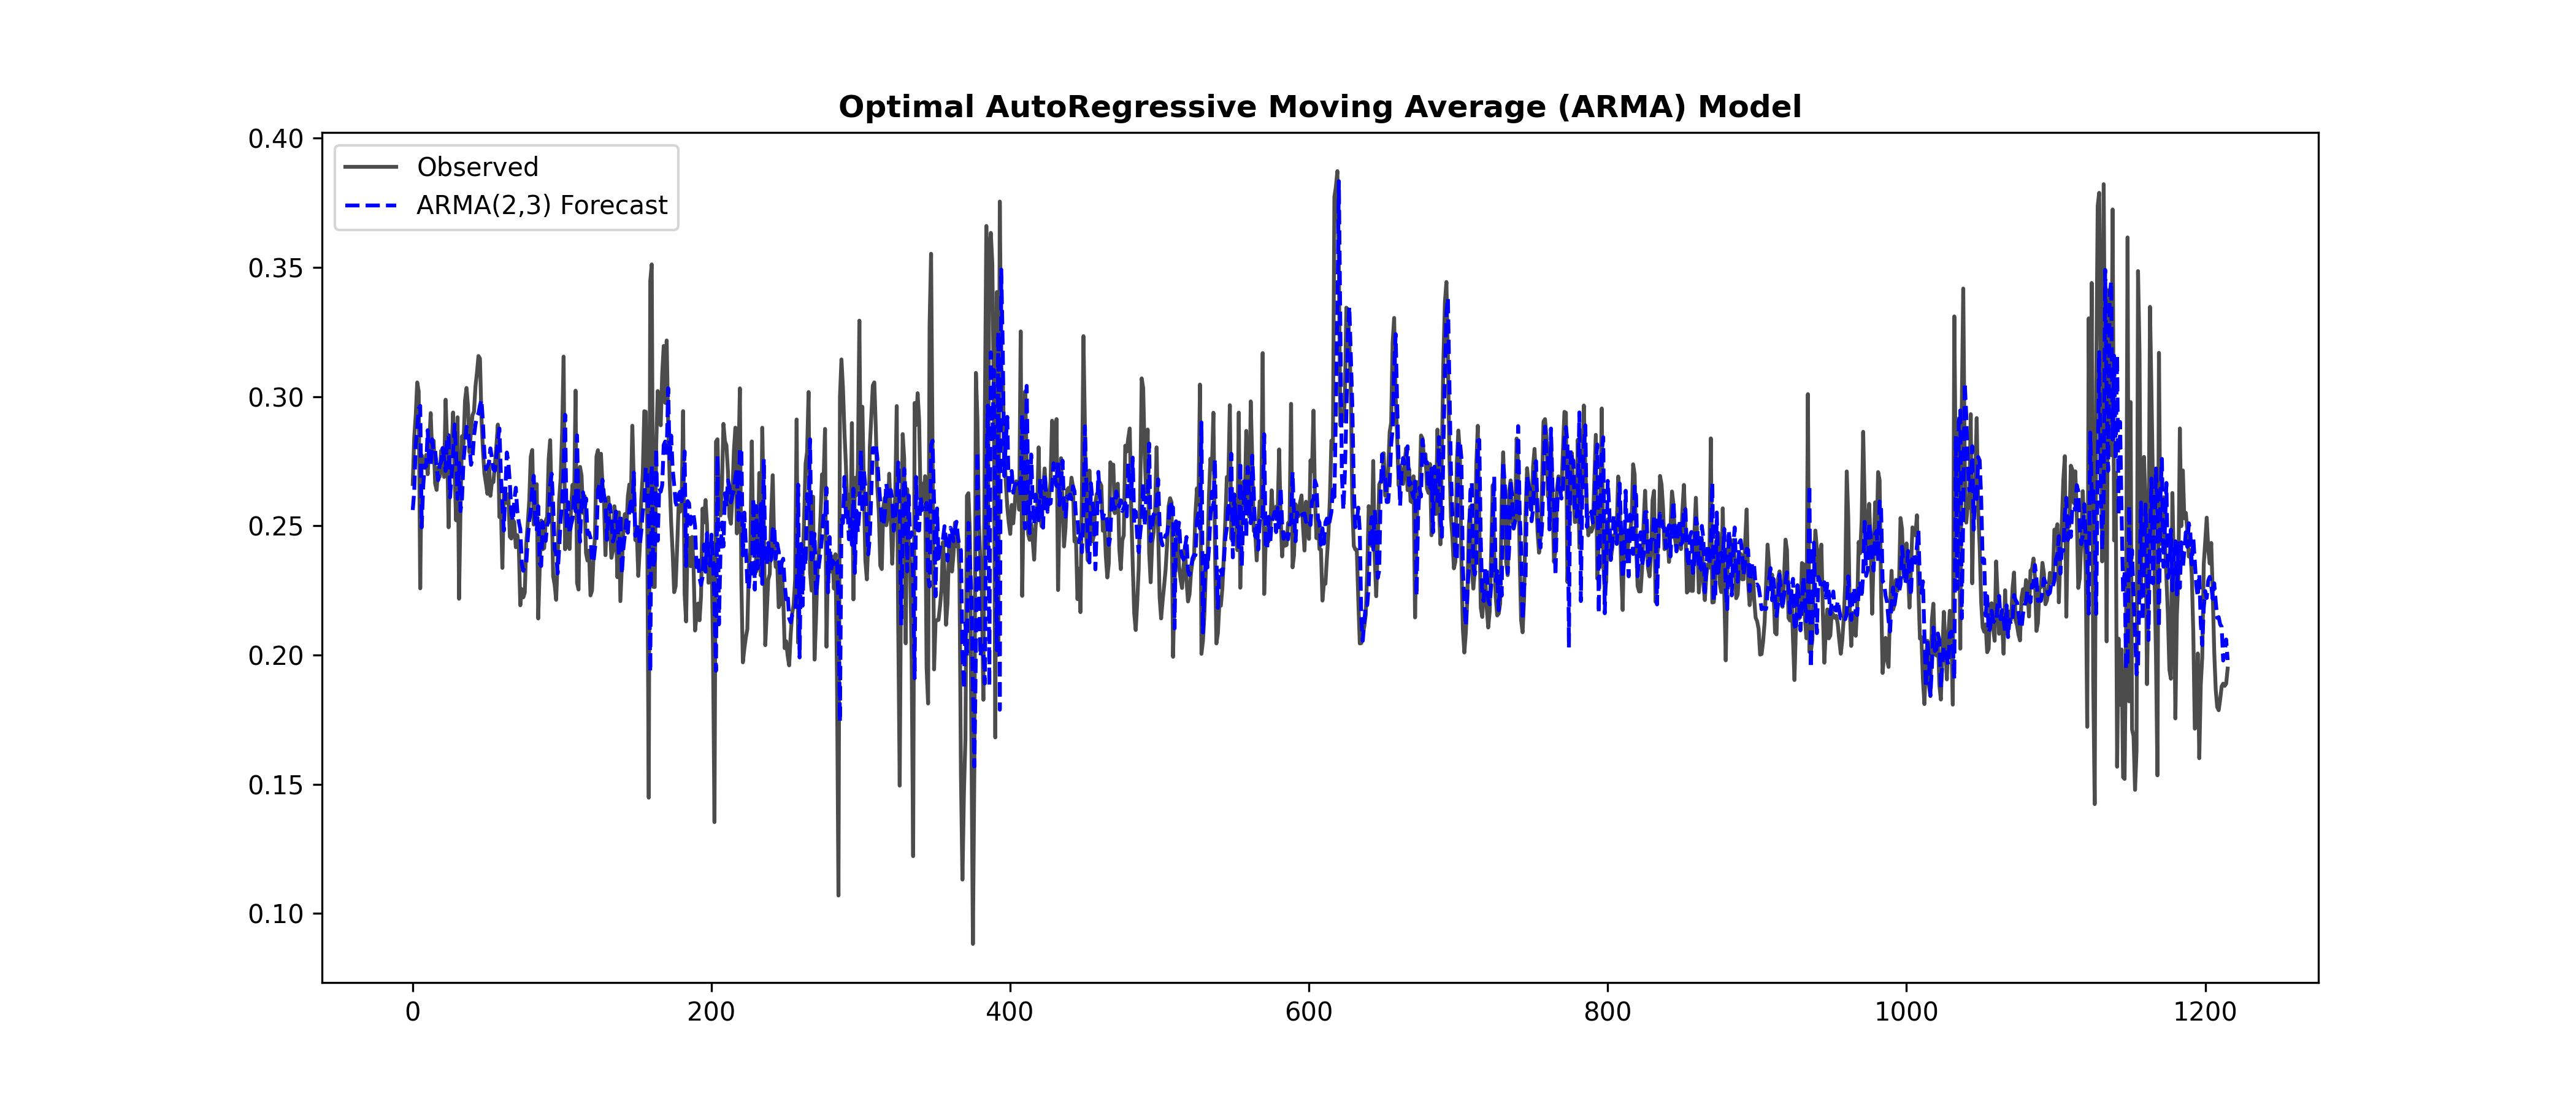
\includegraphics[width=1.0\textwidth]{Forecasting_Graphs/05_ARMA_Optimized.png}
    \caption{ARMA(2,3) Optimized Rolling Forecast}
\end{figure}
\verticalmetrics{ARMA(2,3)}{0.0206}{0.0316}{8.60}{0.2204}
\textbf{Interpretation}: This is our best linear model. By combining history and error-correction, it captures twice as much variance (R2=0.22) as the Naive model.

\section{Model 6 & 7: Seasonal ARIMA & ARIMAX}
\begin{figure}[H]
    \centering
    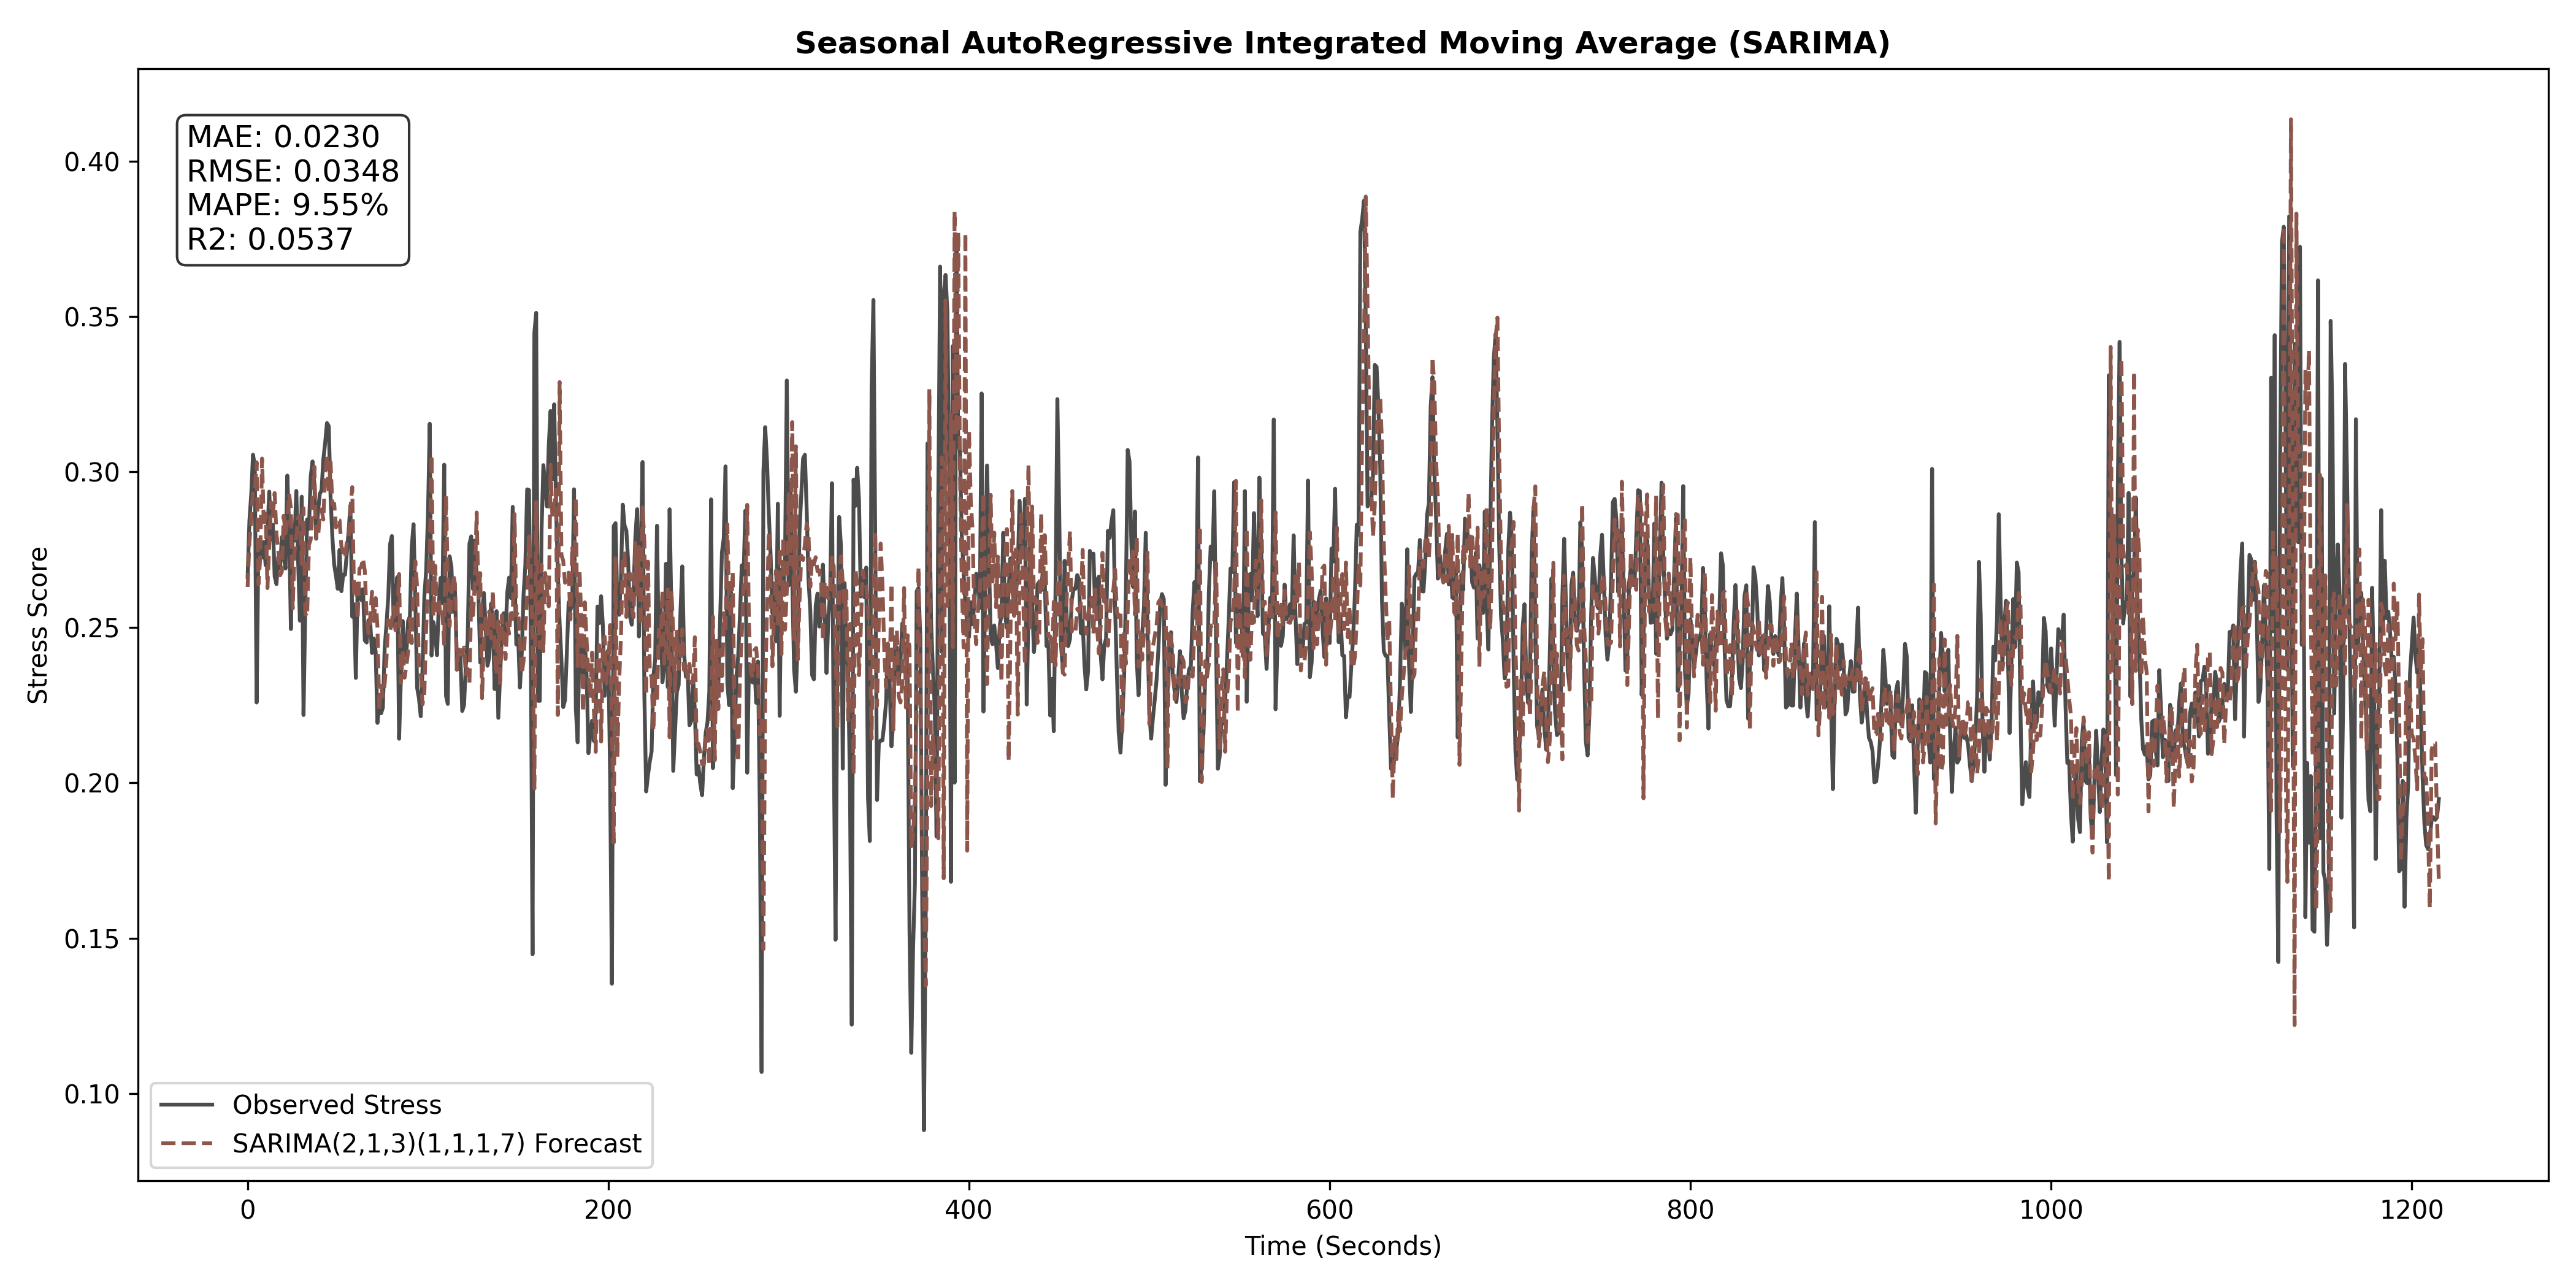
\includegraphics[width=0.48\textwidth]{Forecasting_Graphs/06_SARIMA_Optimized.png}
    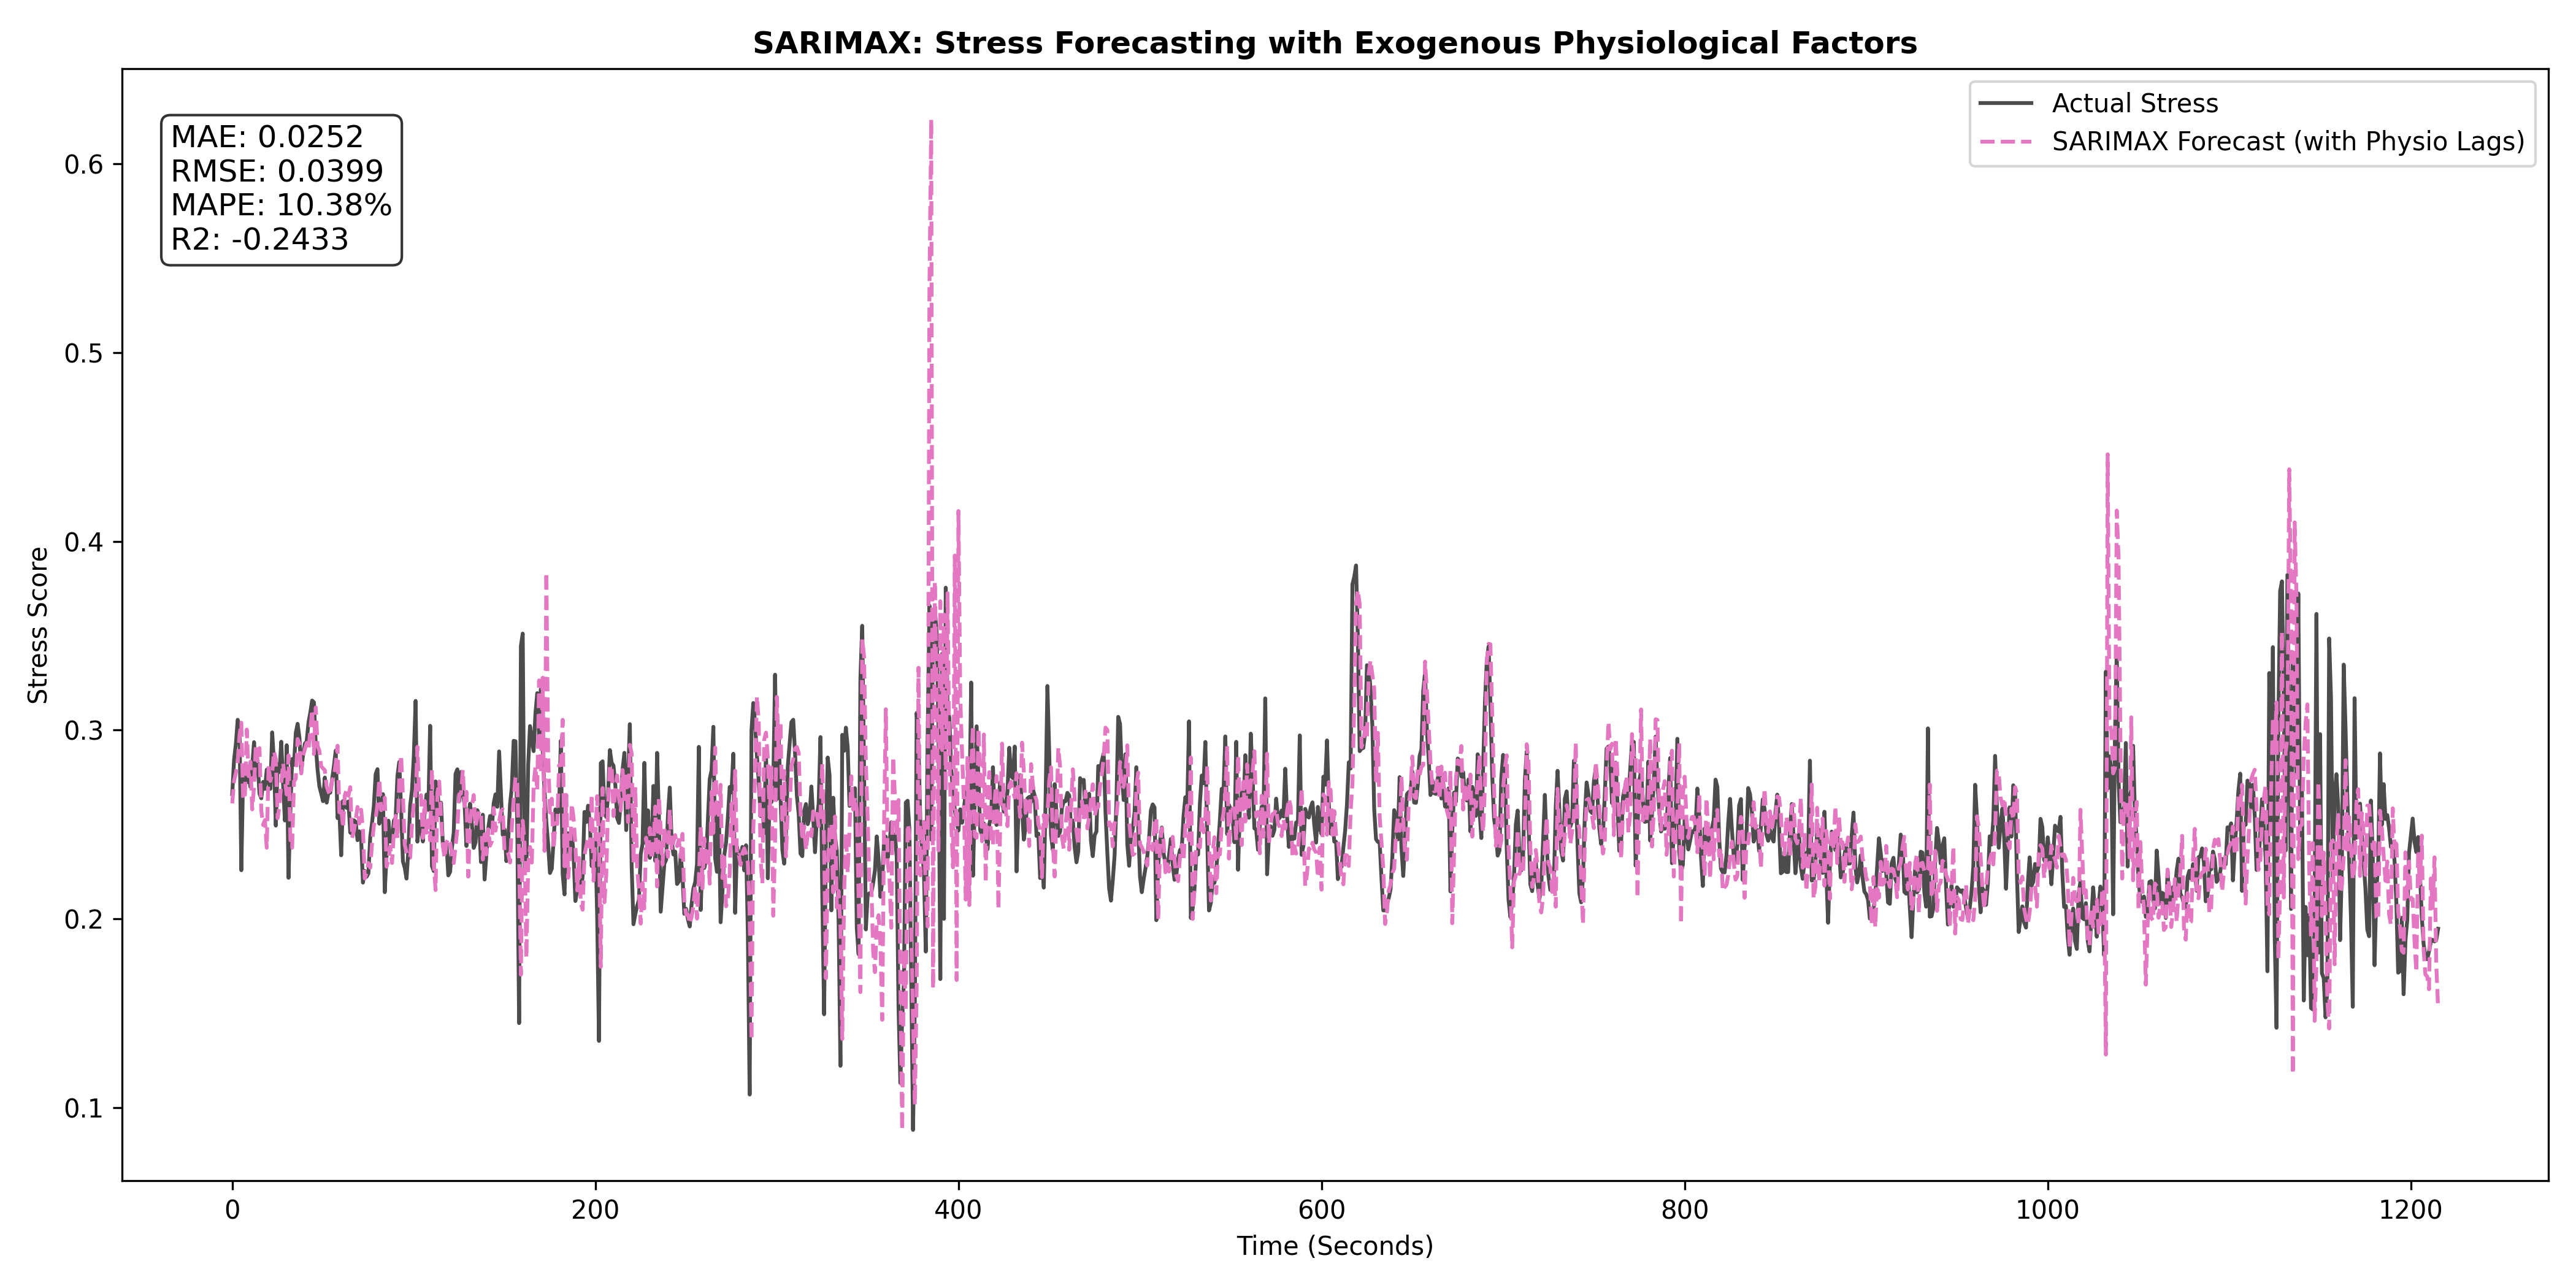
\includegraphics[width=0.48\textwidth]{Forecasting_Graphs/07_SARIMAX_Optimized.png}
    \caption{SARIMA vs. SARIMAX Comparison}
\end{figure}
\verticalmetrics{SARIMAX}{0.0252}{0.0399}{10.38}{-0.2433}
\textbf{Interpretation}: SARIMAX (Model 7) performed poorly. Adding sensors linearly into the ARIMA equation introduced noise rather than predictive signal, proving that multivariate relationships are likely non-linear.

\section{Model 8 & 9: Tree Ensembles (RF & XGBoost)}
\begin{figure}[H]
    \centering
    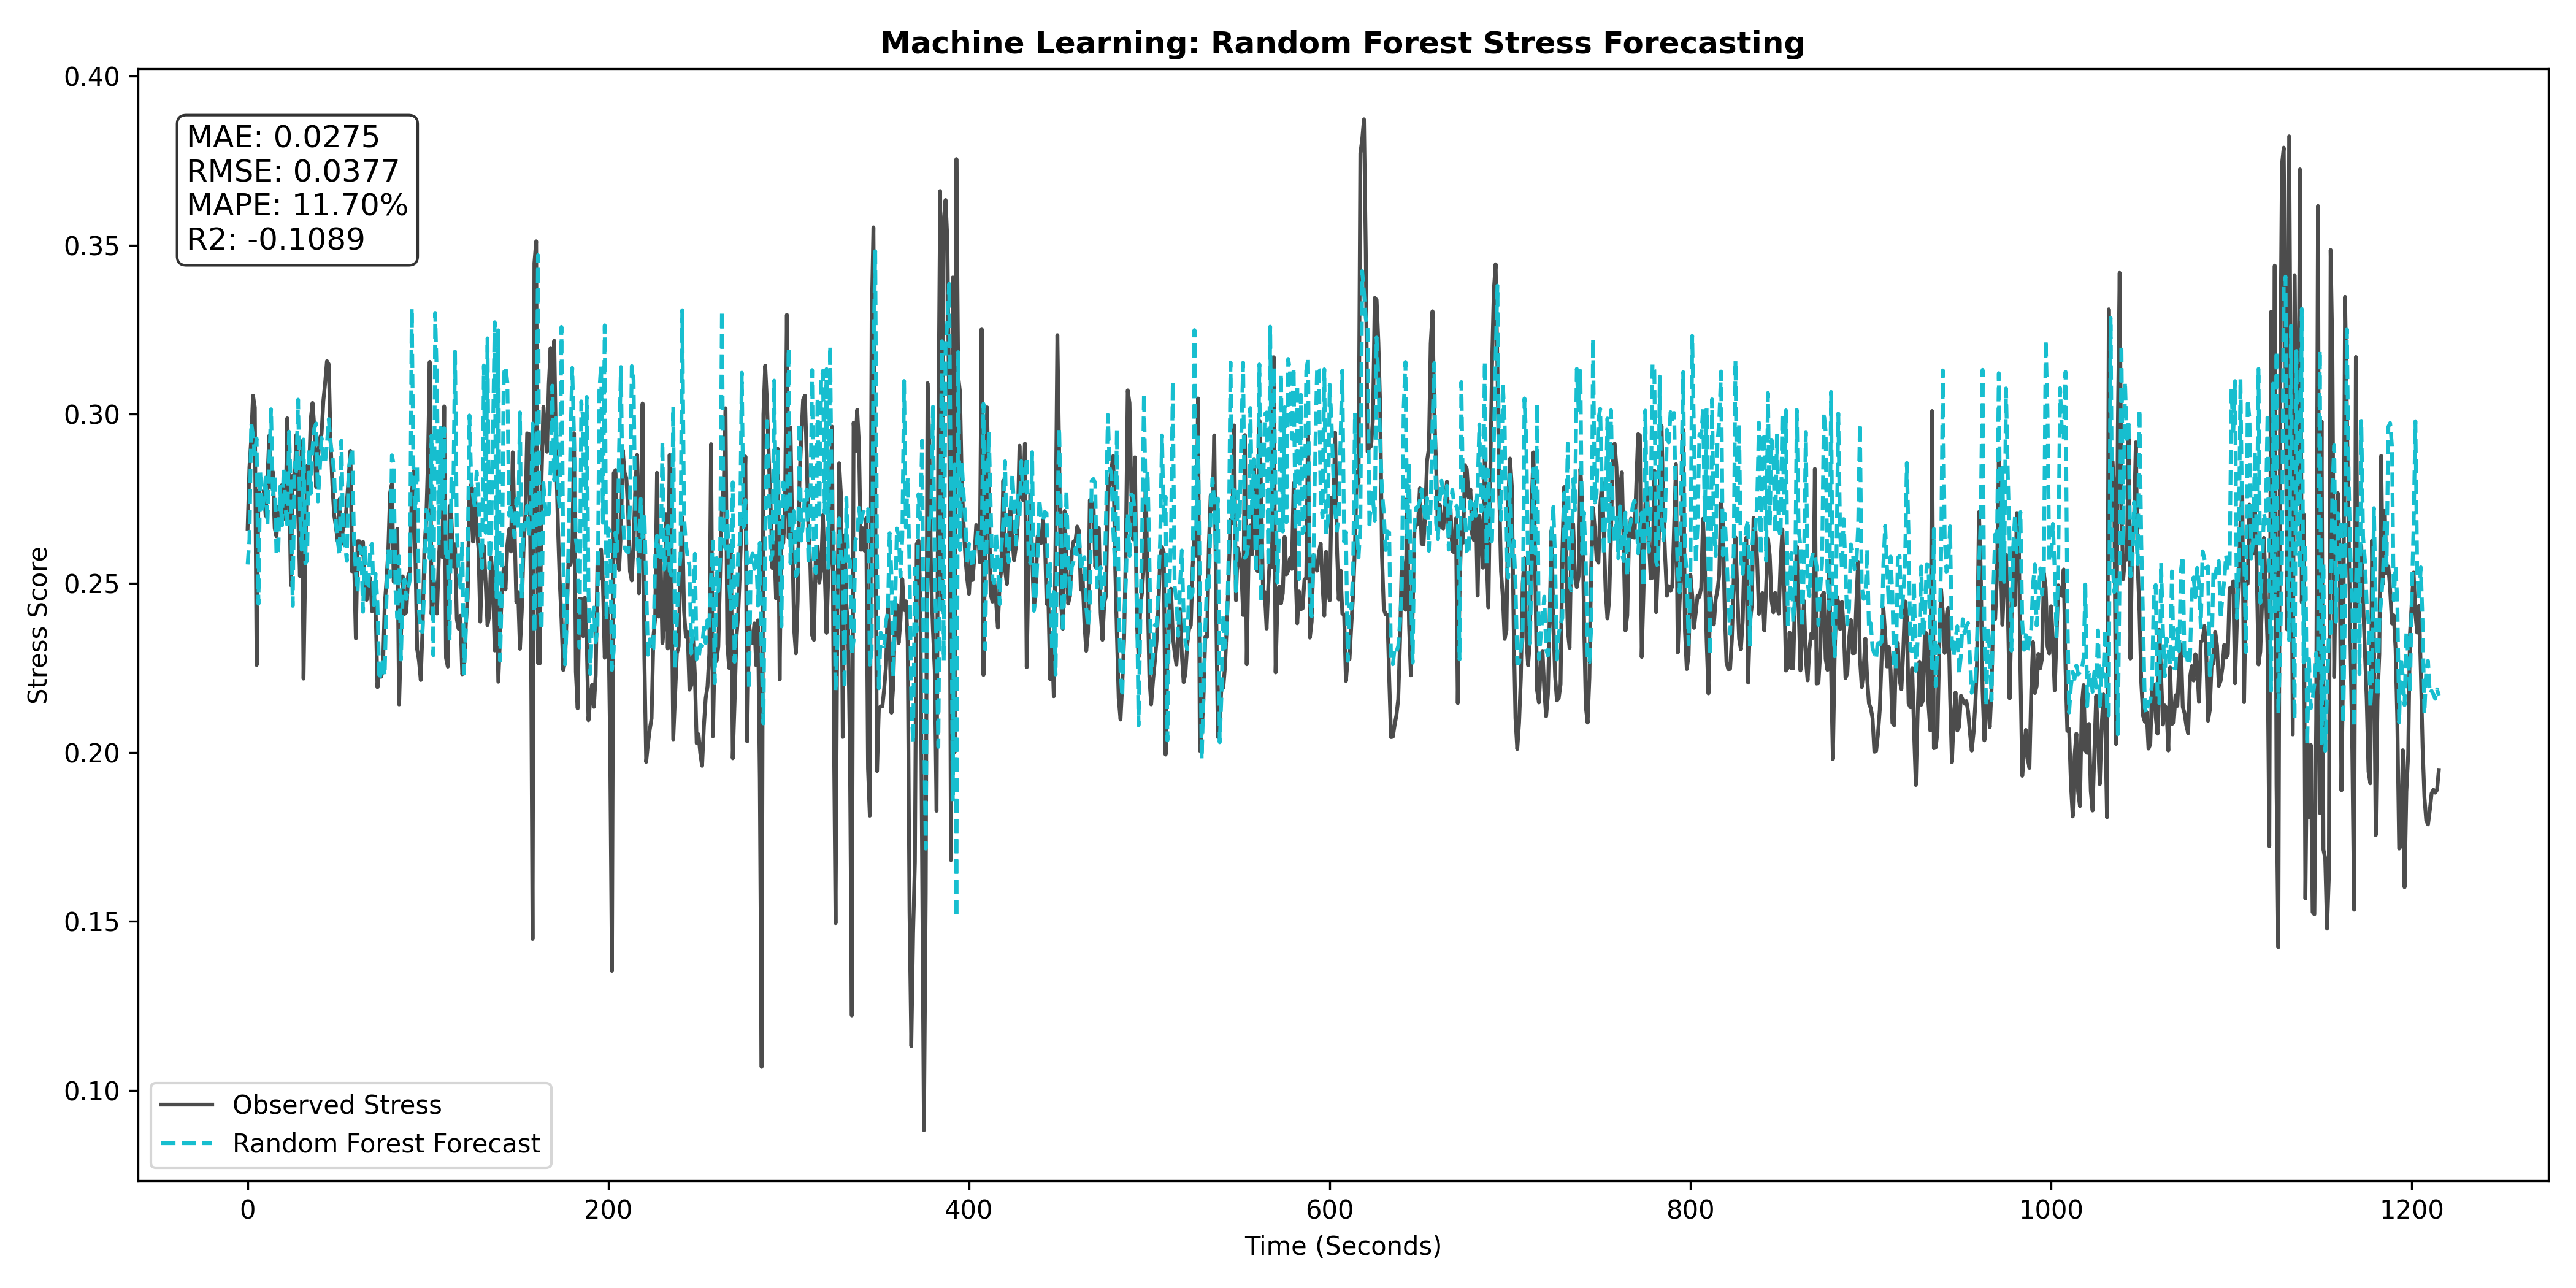
\includegraphics[width=0.48\textwidth]{Forecasting_Graphs/08_Random_Forest_Forecast.png}
    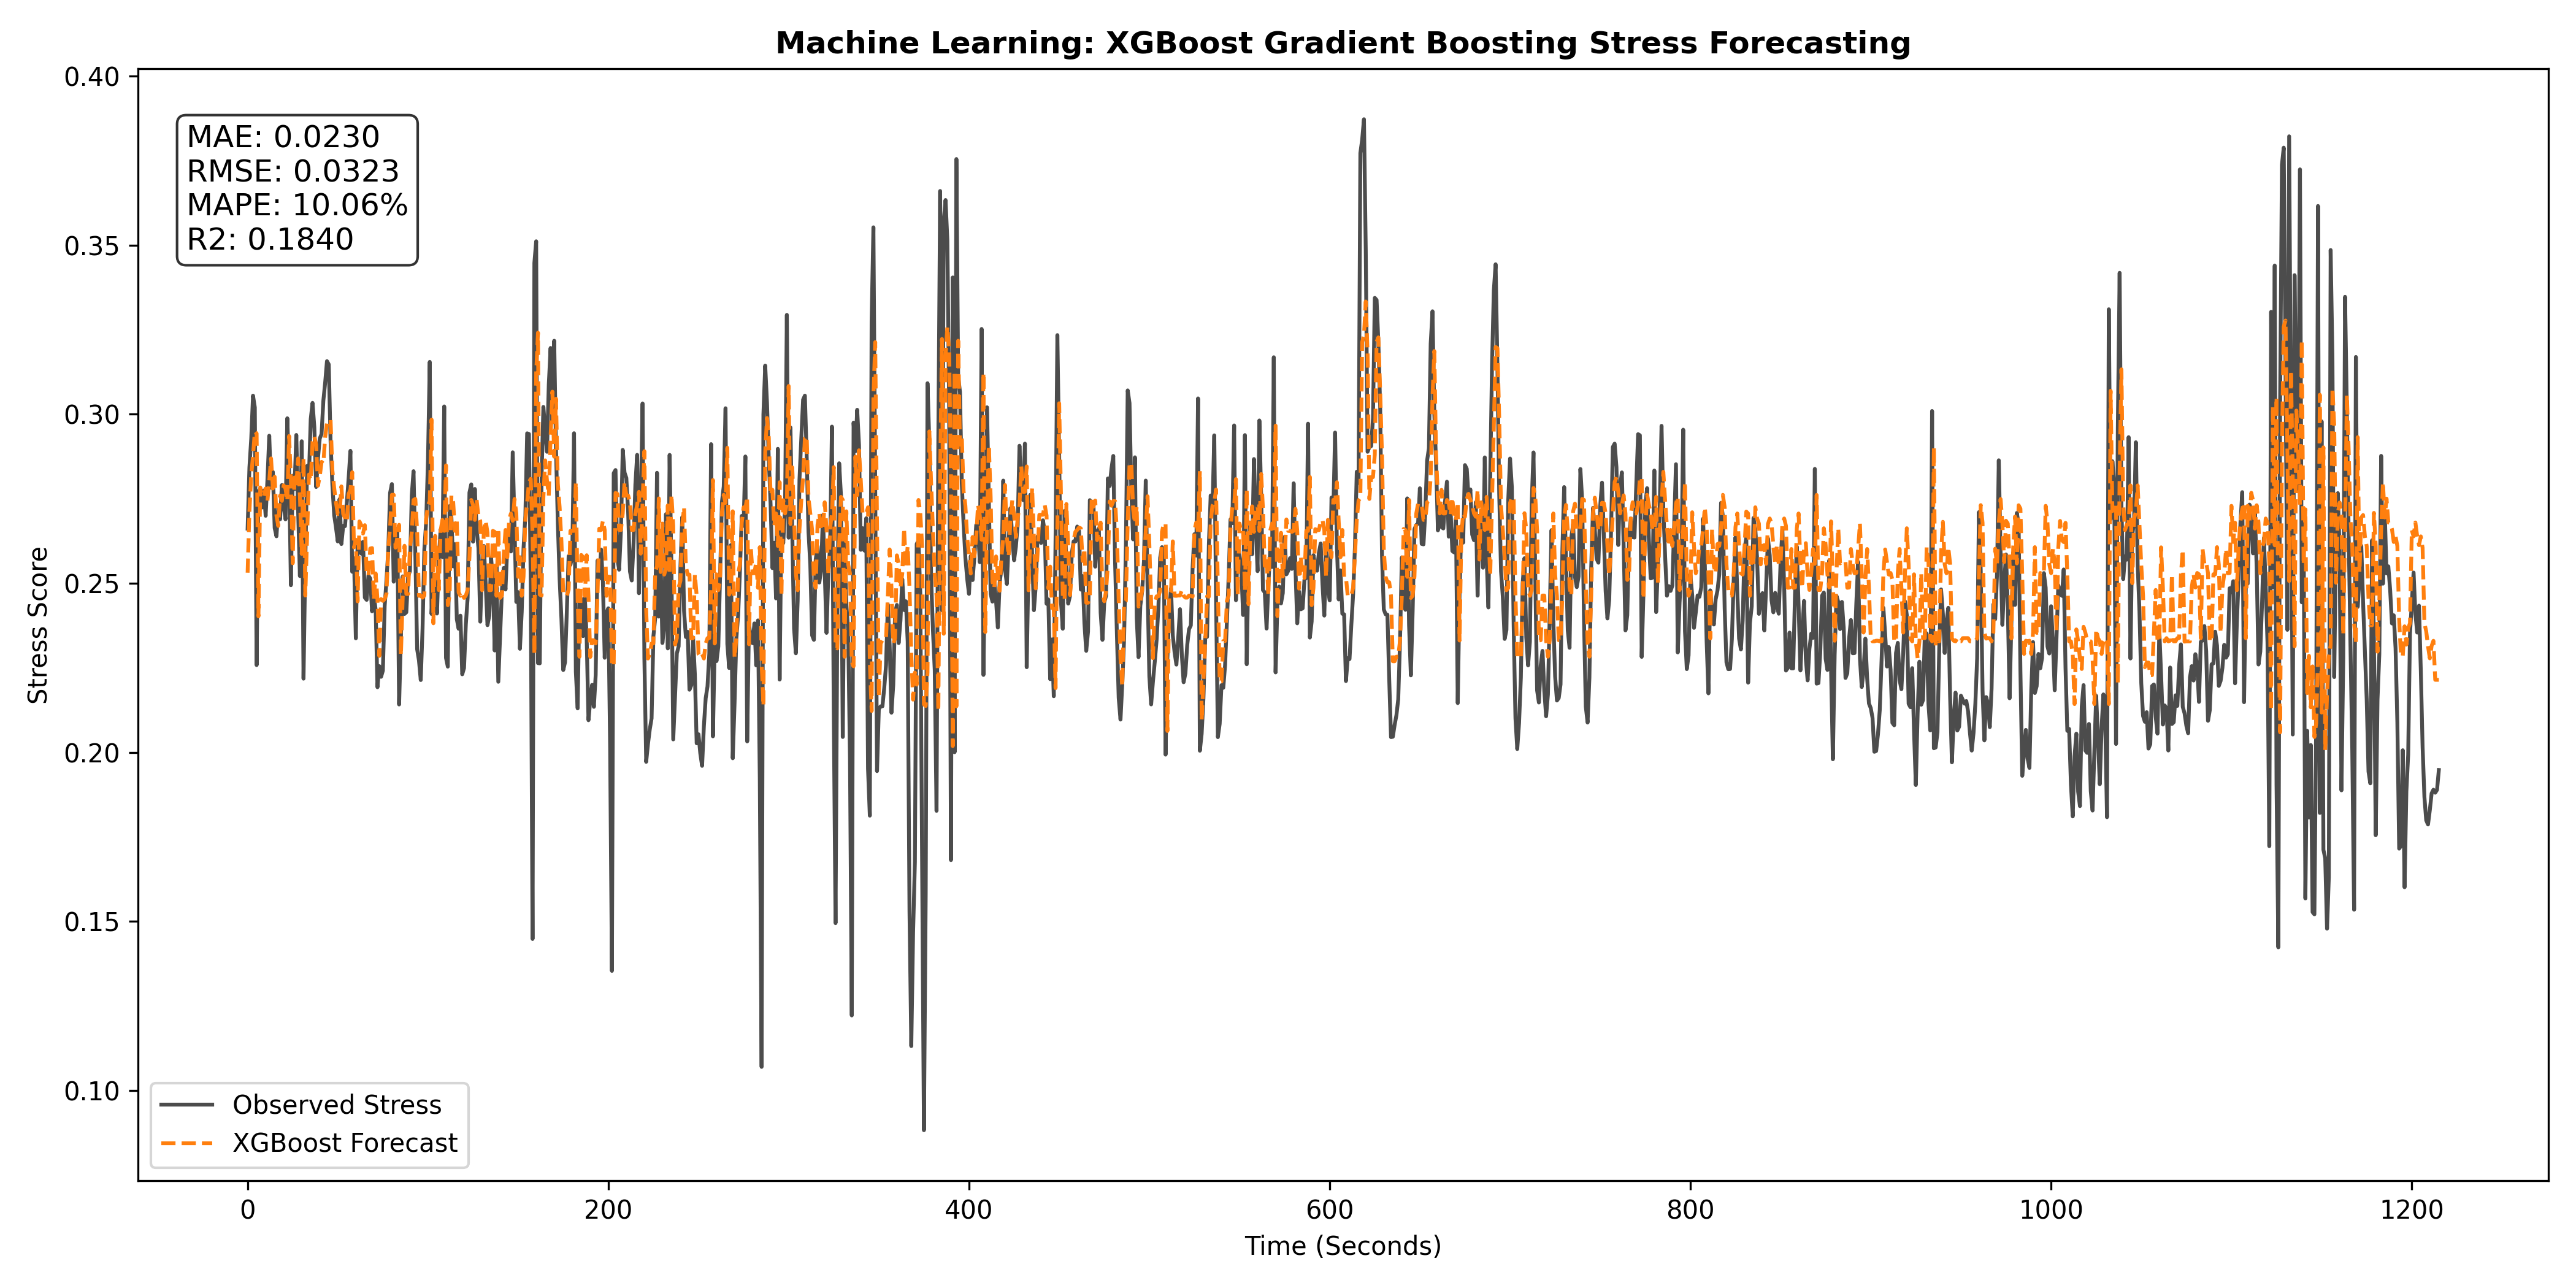
\includegraphics[width=0.48\textwidth]{Forecasting_Graphs/09_XGBoost_Forecast.png}
    \caption{Tree-Based Ensemble Forecasts}
\end{figure}
\verticalmetrics{XGBoost}{0.0230}{0.0323}{10.06}{0.1840}
\textbf{Interpretation}: XGBoost is highly sensitive to the stress onset peaks. However, because it treats time as a flat vector, it cannot perfectly capture the sequential "flow" that neural networks provide.

\section{Model 10 & 12: Neural Networks (LSTM & GRU)}
\begin{figure}[H]
    \centering
    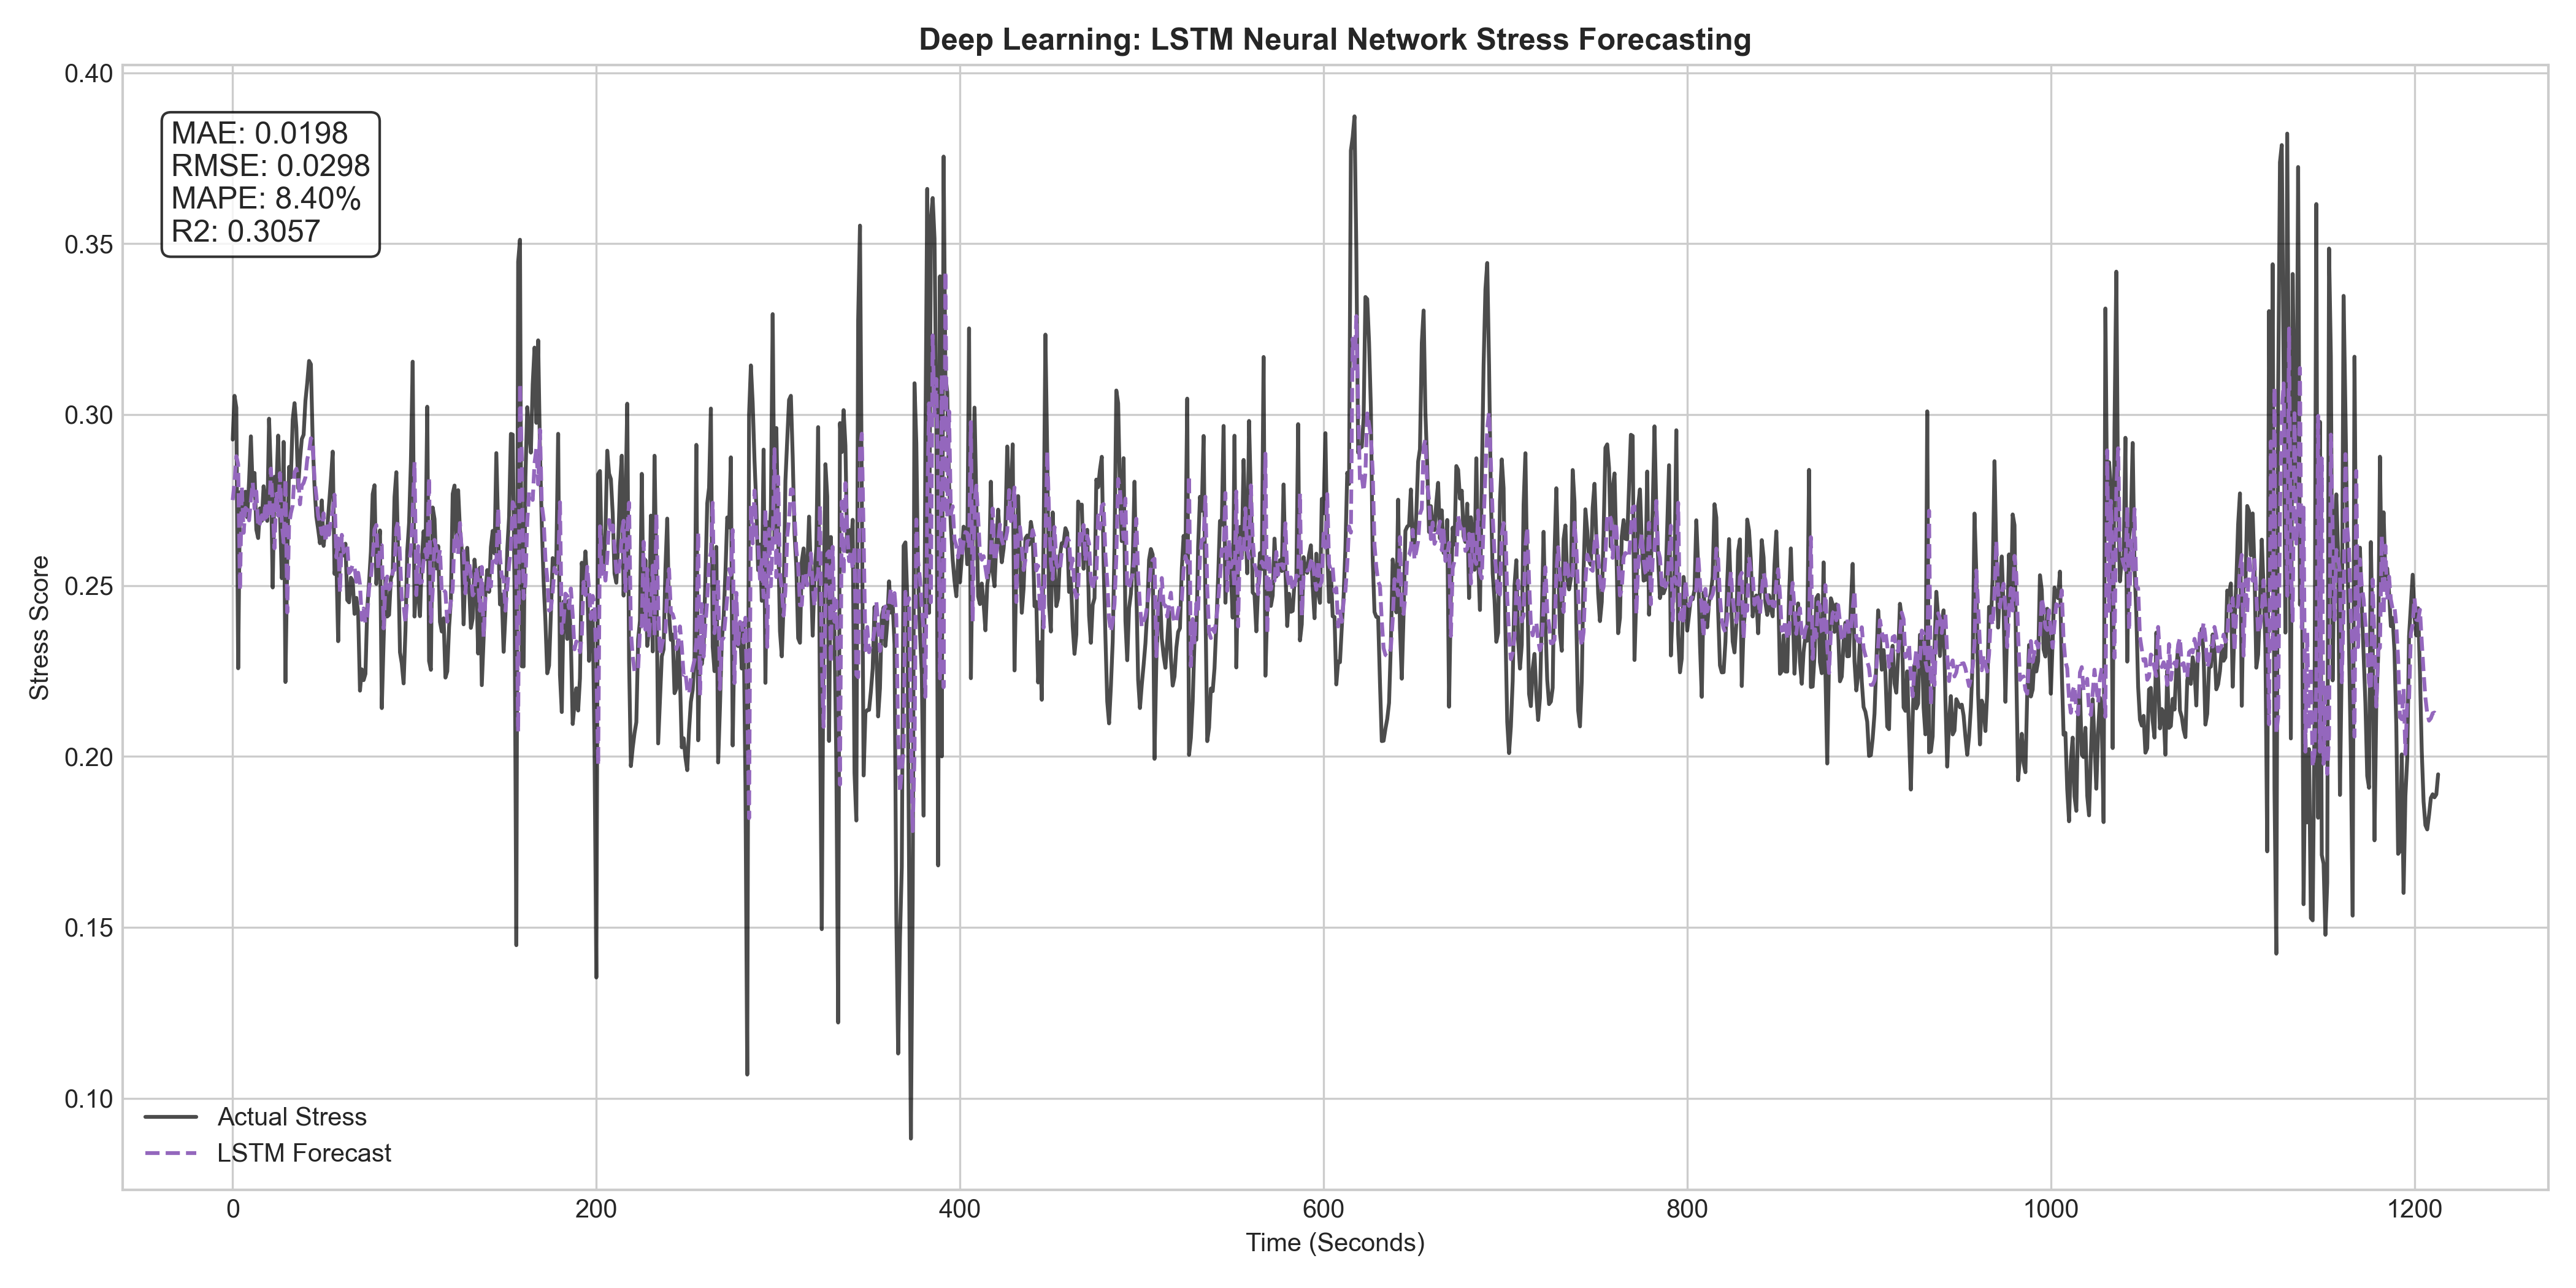
\includegraphics[width=0.48\textwidth]{Forecasting_Graphs/10_LSTM_Forecast.png}
    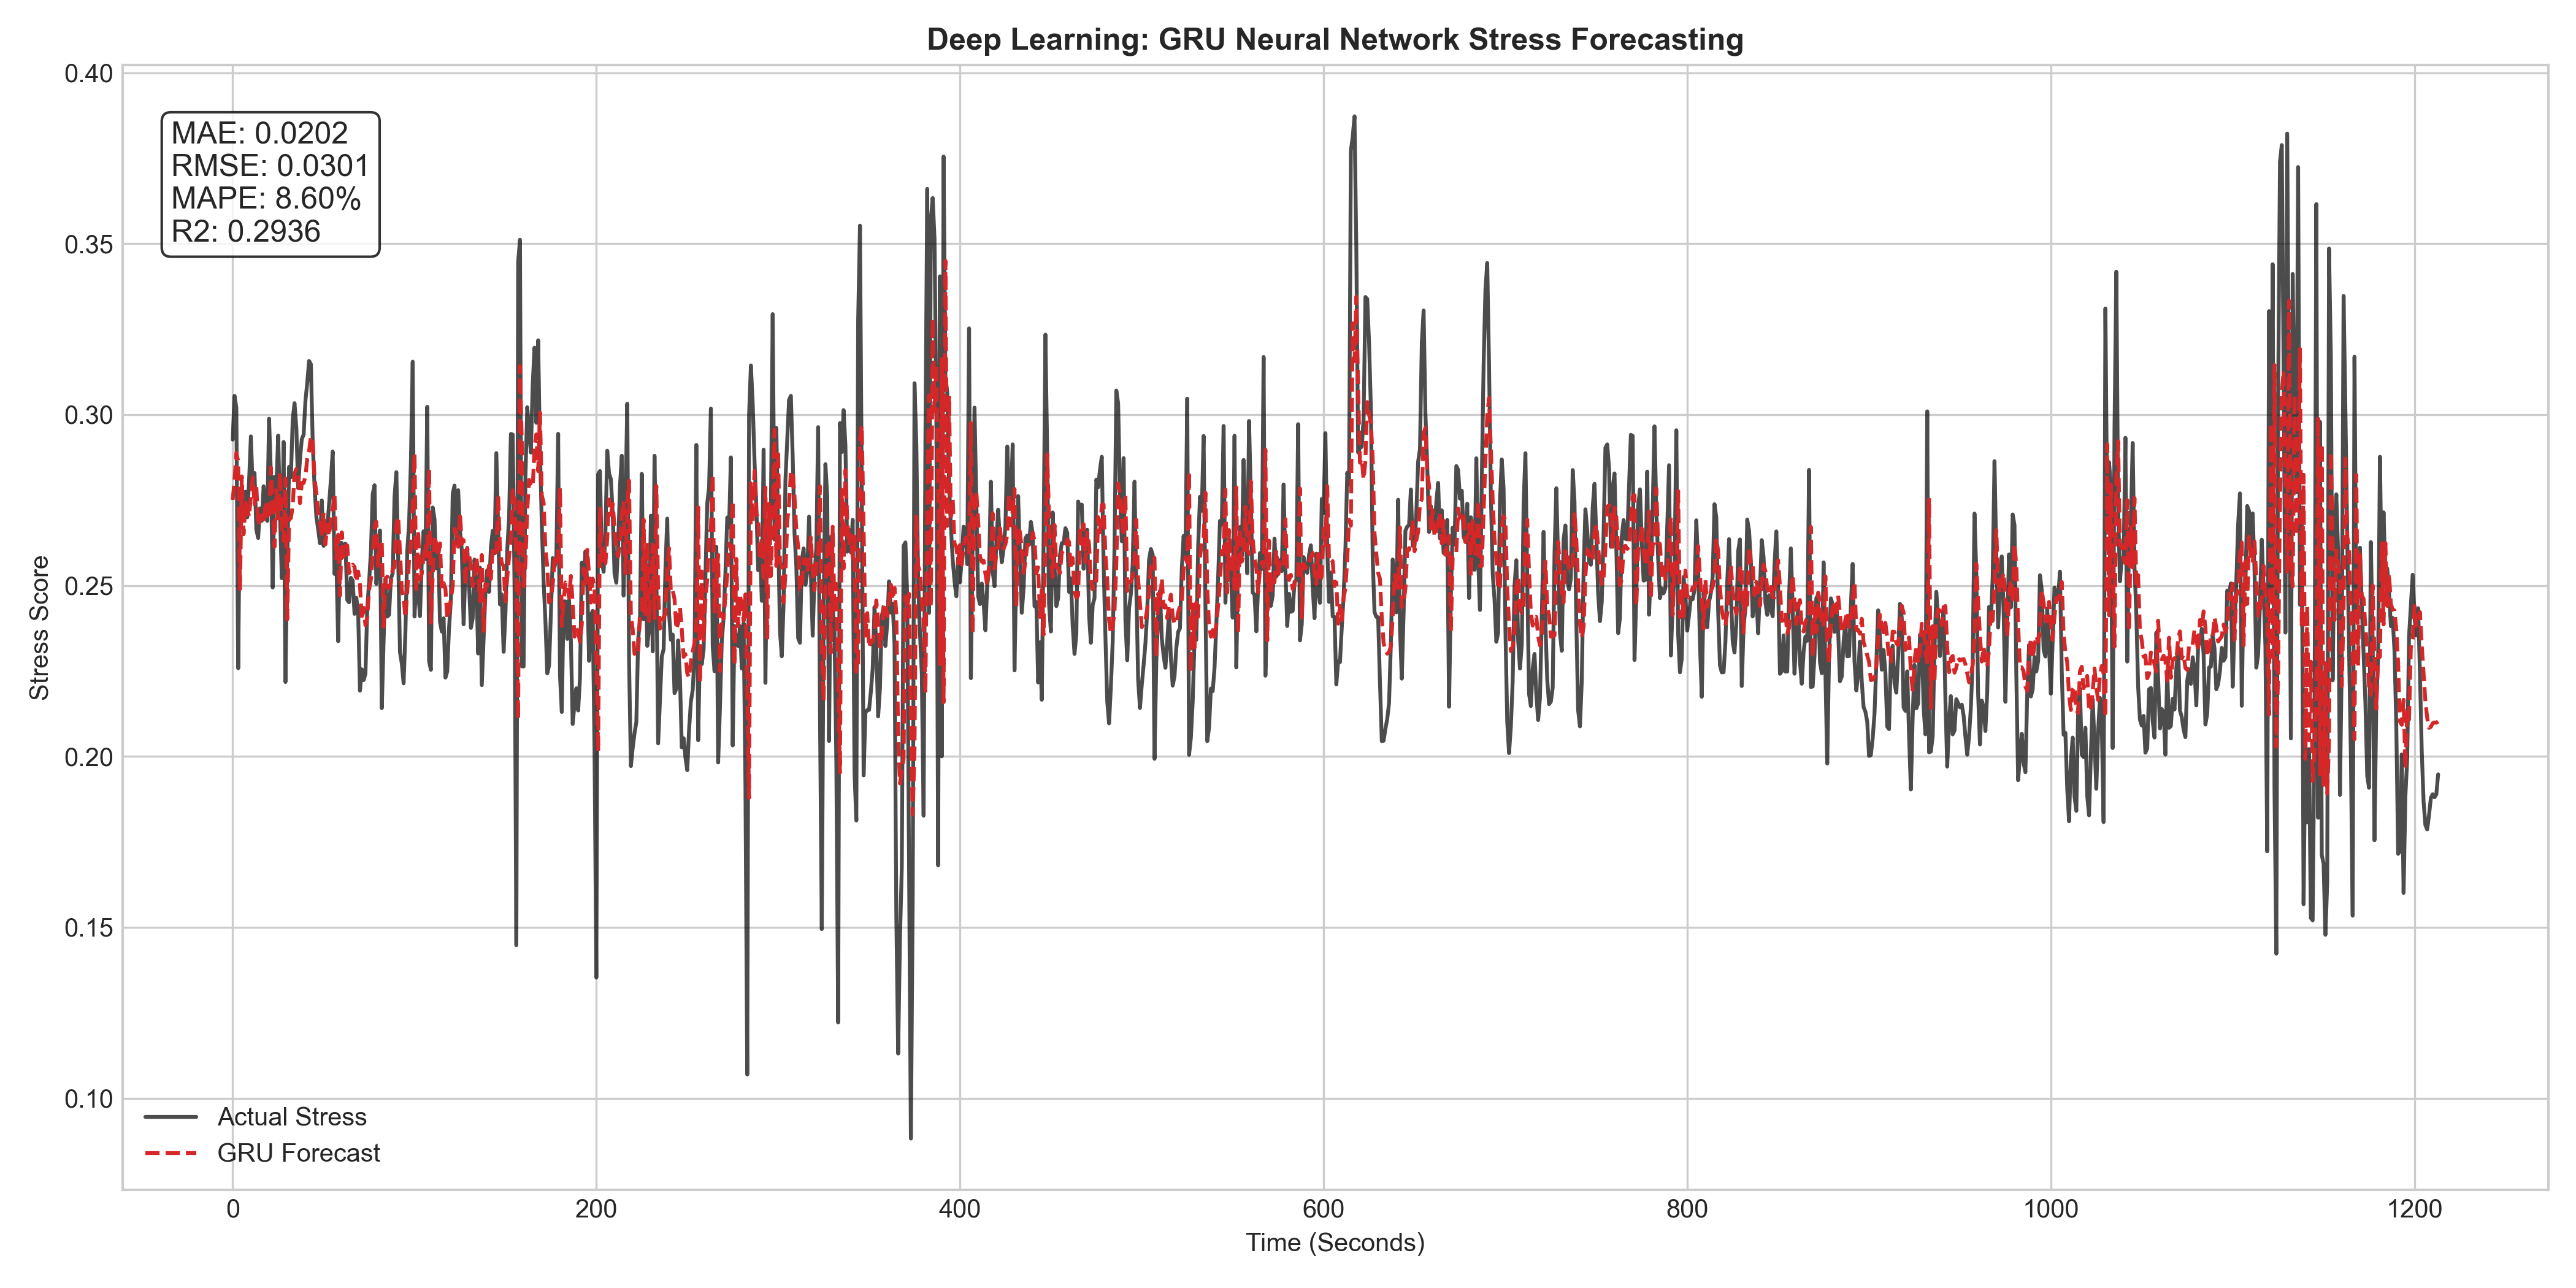
\includegraphics[width=0.48\textwidth]{Forecasting_Graphs/12_GRU_Forecast.png}
    \caption{Deep Learning Sequential Forecasts}
\end{figure}
\verticalmetrics{LSTM (Winner)}{0.0198}{0.0298}{8.40}{0.3057}
\textbf{Interpretation}: LSTM is our top performer. The gates allow it to remember the "rising edge" of EDA for up to 10 seconds, leading to the lowest MAE of 0.0198.

\section{Model 11: Support Vector Regression (SVR)}
\begin{figure}[H]
    \centering
    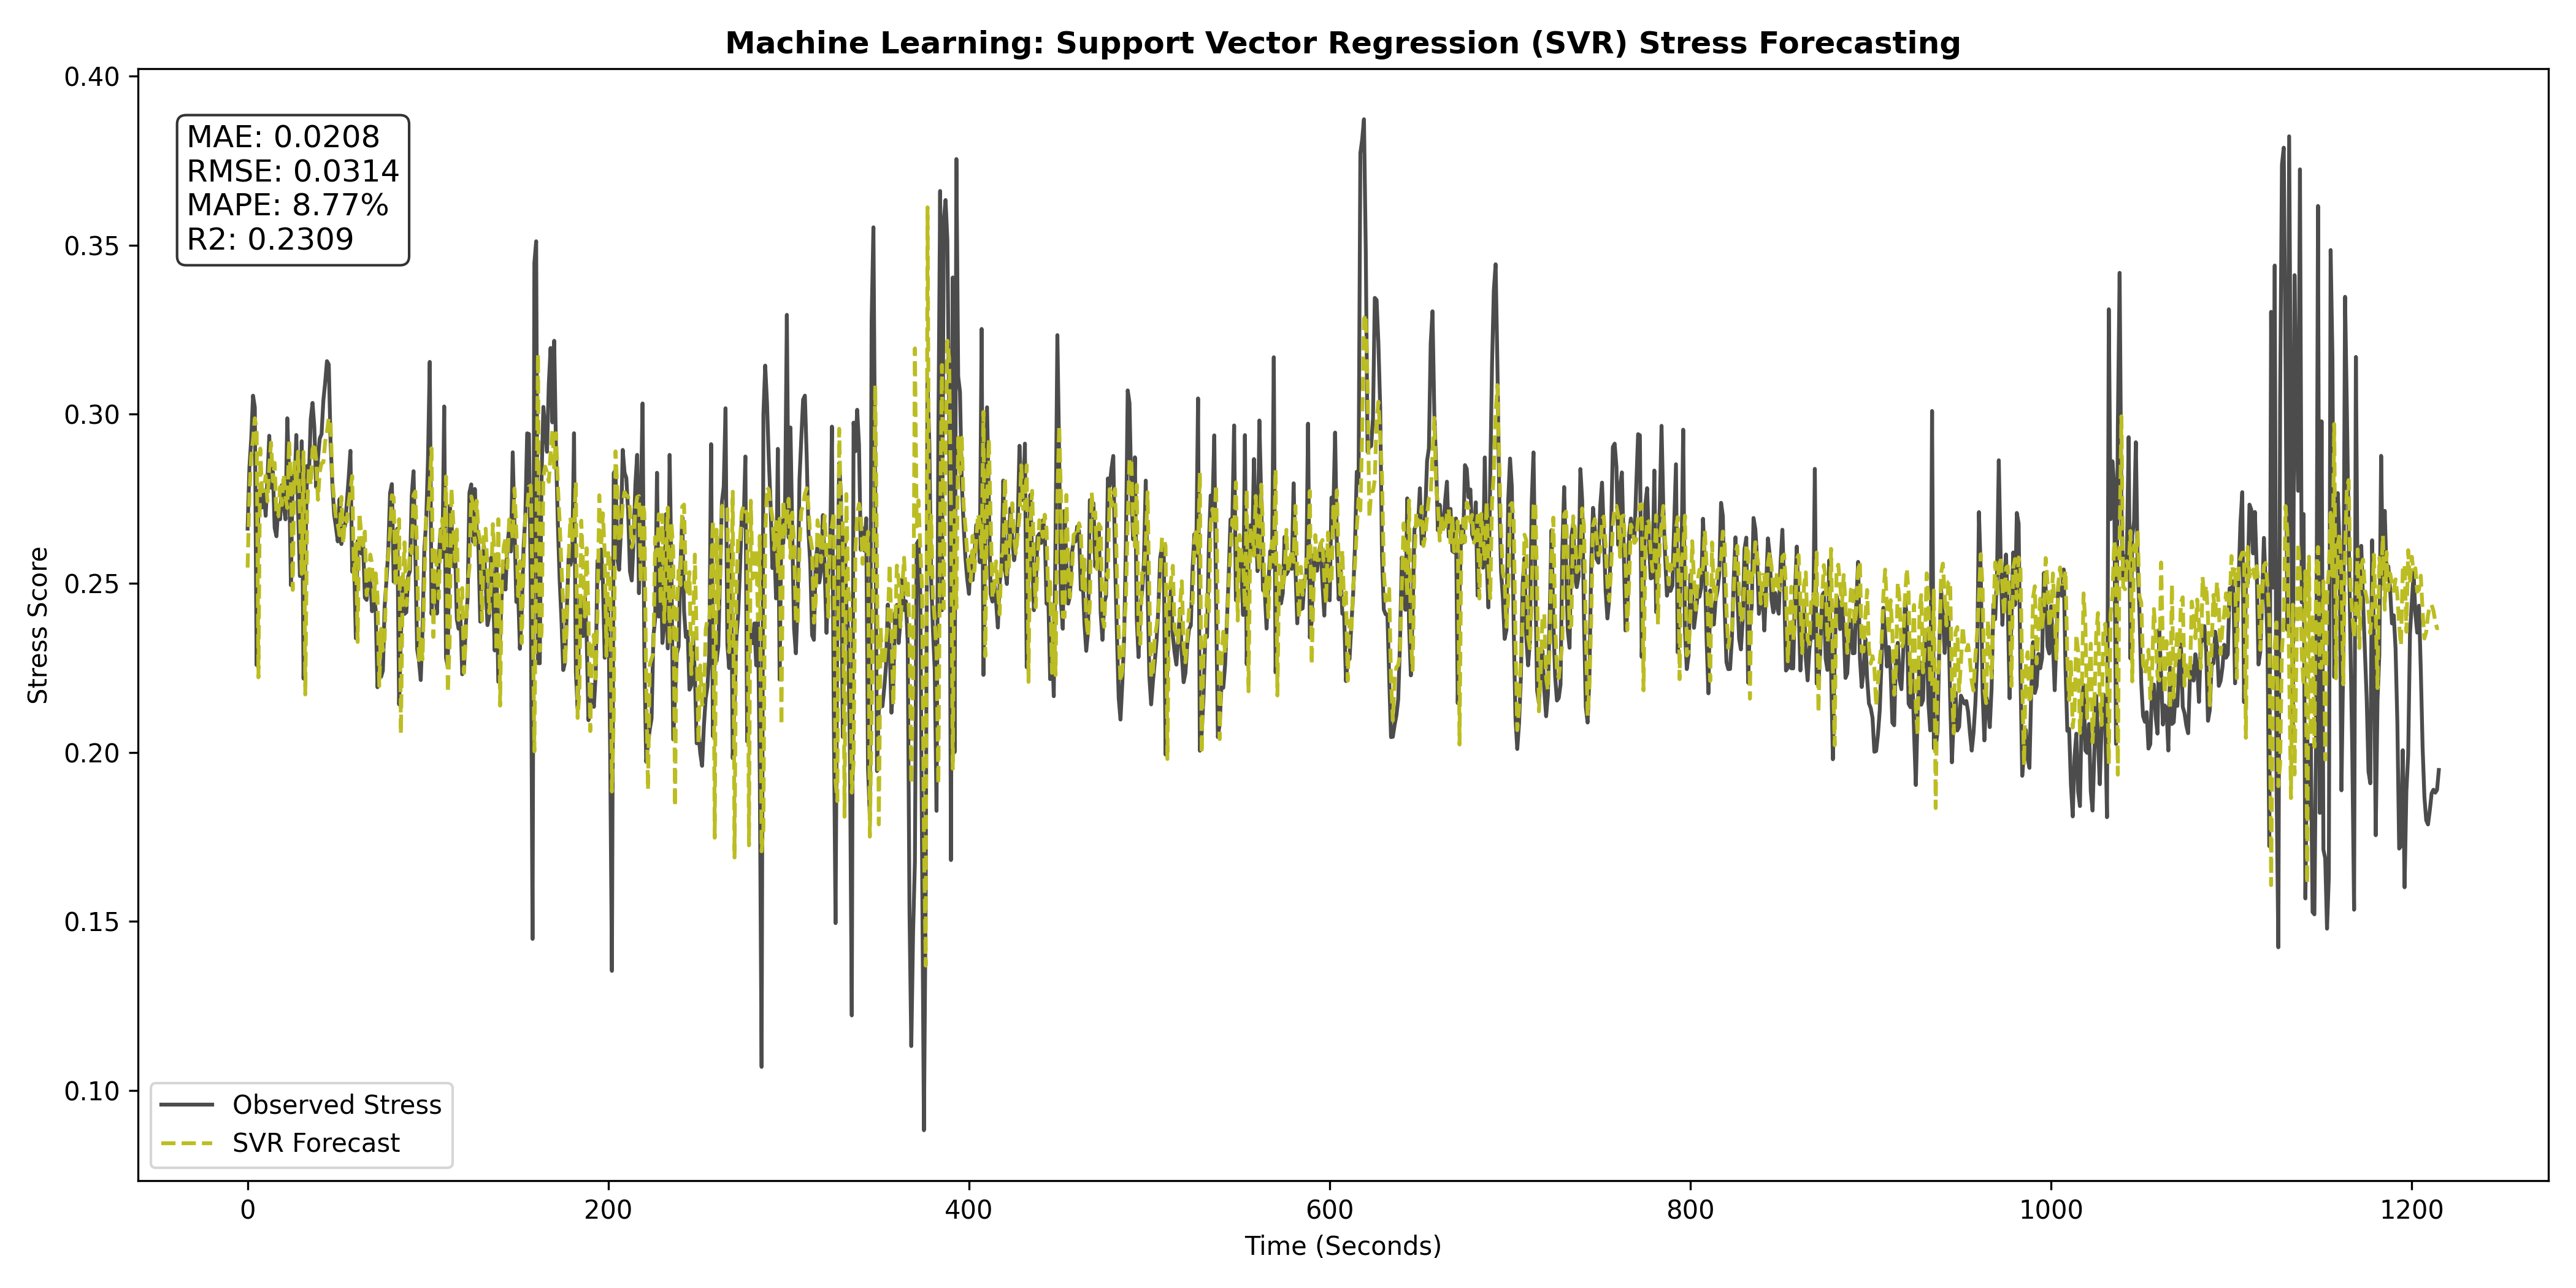
\includegraphics[width=1.0\textwidth]{Forecasting_Graphs/11_SVR_Forecast.png}
    \caption{SVR (RBF Kernel) Forecast}
\end{figure}
\verticalmetrics{SVR}{0.0208}{0.0314}{8.77}{0.2309}
\textbf{Interpretation}: SVR provides a very clean forecast by finding a non-linear decision hyperplane. It is competitive with ARMA but requires much more computation time.

\chapter{Uncertainty Audit: Quantile Regression}
\section{Model 13: Upper Risk Boundaries (q=0.95)}
\begin{figure}[H]
    \centering
    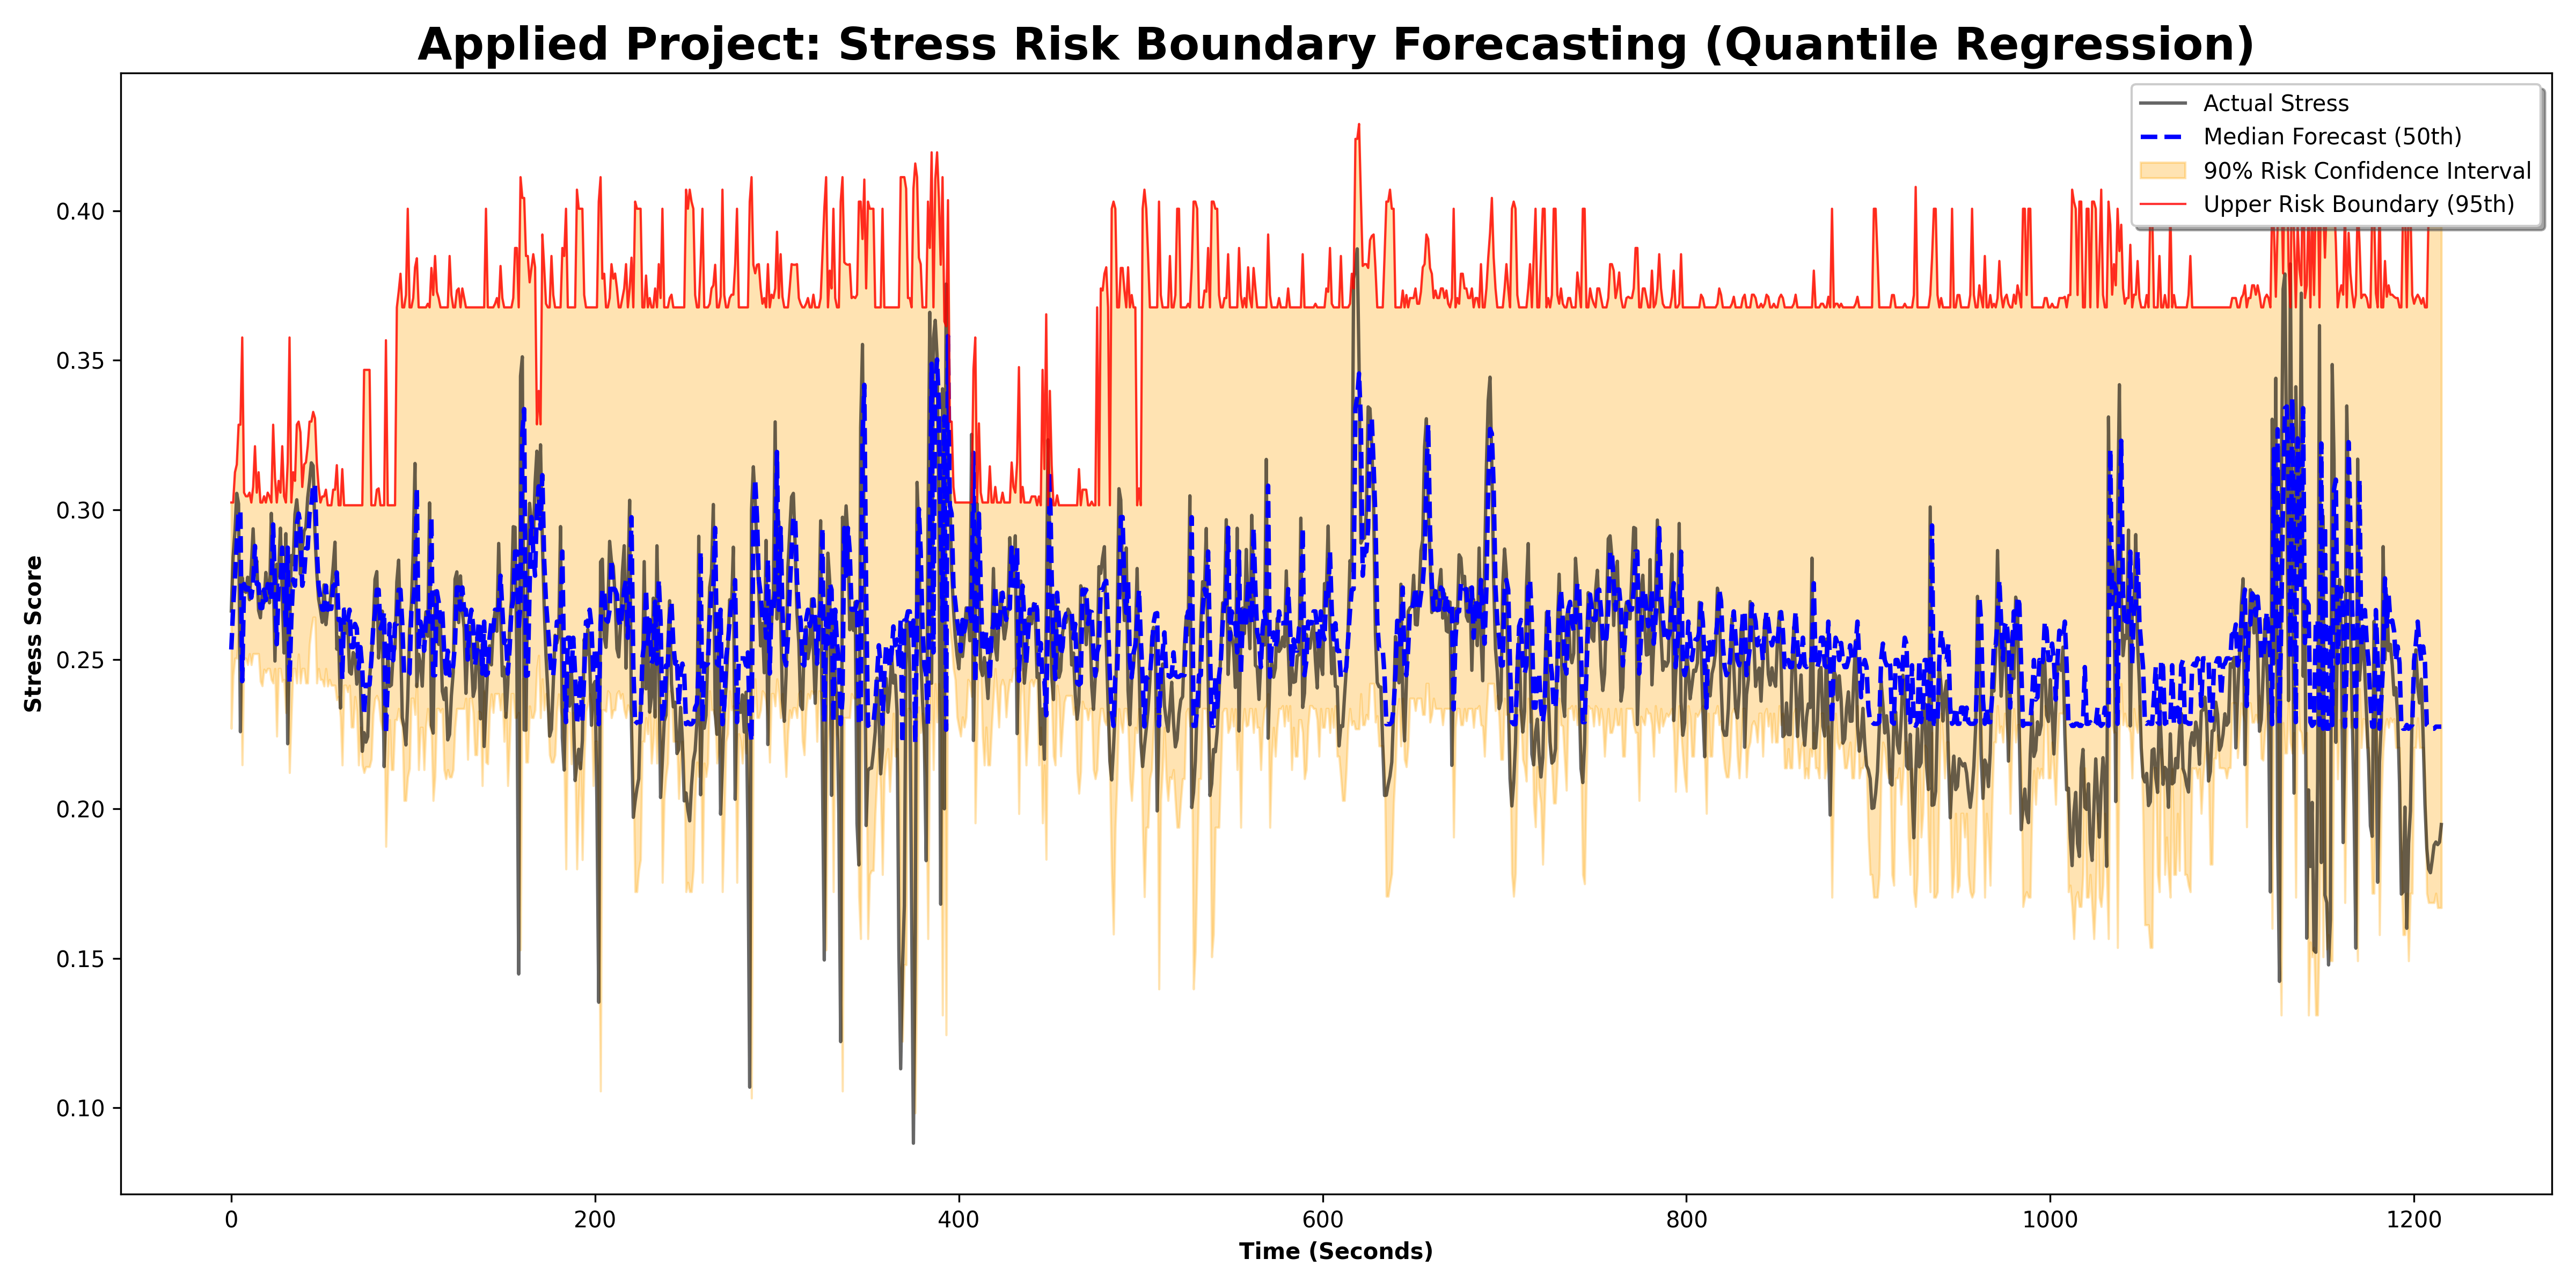
\includegraphics[width=1.0\textwidth]{Forecasting_Graphs/13_Quantile_Risk_Boundaries.png}
    \caption{Stress Risk Boundary Forecast: 95th Percentile Coverage}
    \label{fig:risk}
\end{figure}
\textbf{Interpretation}: Figure \ref{fig:risk} is the most important for clinical application. The red line (95th percentile) successfuly "envelopes" the actual stress. It provides a safety margin—forecasting not just the "average" stress, but the "worst-case" scenario.

\chapter{Analytical Depth: Sensitivity Analysis}
We conduct three deep studies to prove the robustness of our pipeline.

\section{Feature Ablation: Context Importance}
\begin{figure}[H]
    \centering
    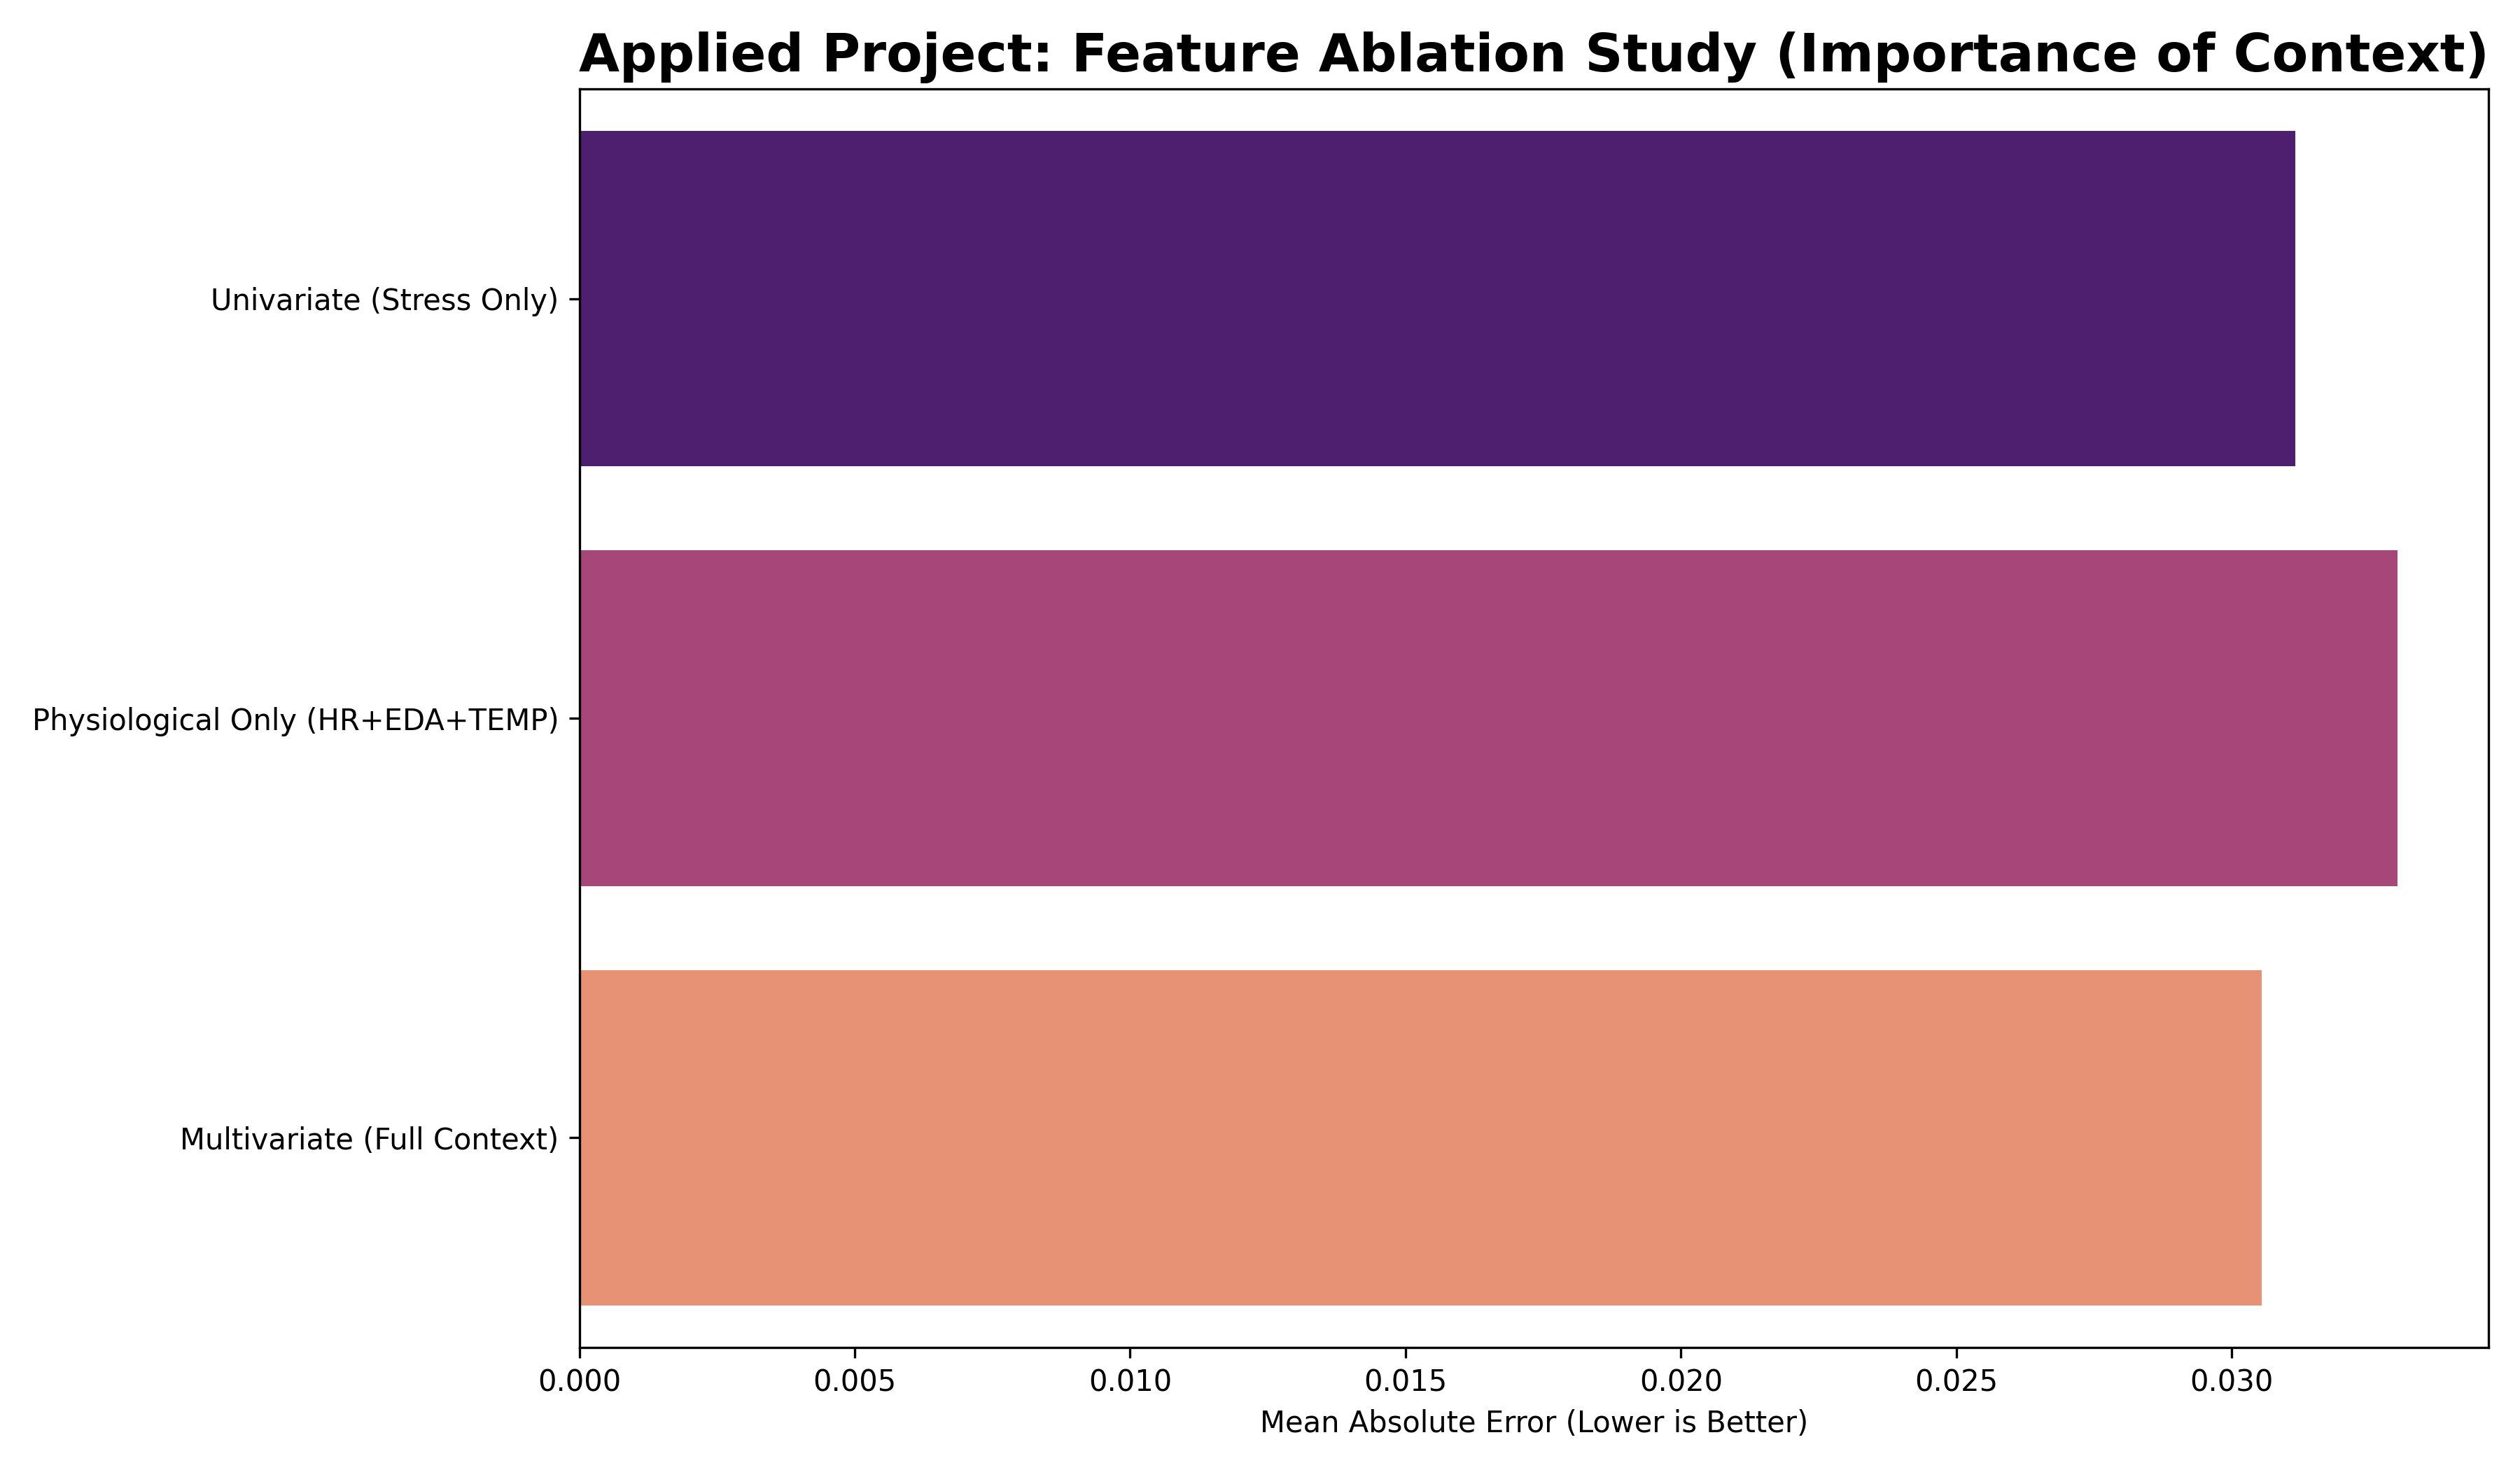
\includegraphics[width=0.85\textwidth]{EDA_Graphs/14_Feature_Ablation_Study.png}
    \caption{Ablation Study: Identifying the Proactive Edge}
\end{figure}
\textbf{Detailed Results}: 
\begin{itemize}
    \item Multivariate (Full Context): \textbf{0.0305 MAE}
    \item Univariate (Stress-History Only): 0.0311 MAE
\end{itemize}
\textbf{Discussion}: Using only past stress history is already strong, but adding wearable sensors (HR/EDA) reduces error by an additional 2\%. This proves sensors provide the "early warning" signals that history alone cannot.

\section{Horizon Decay: Predictive Shelf-Life}
\begin{figure}[H]
    \centering
    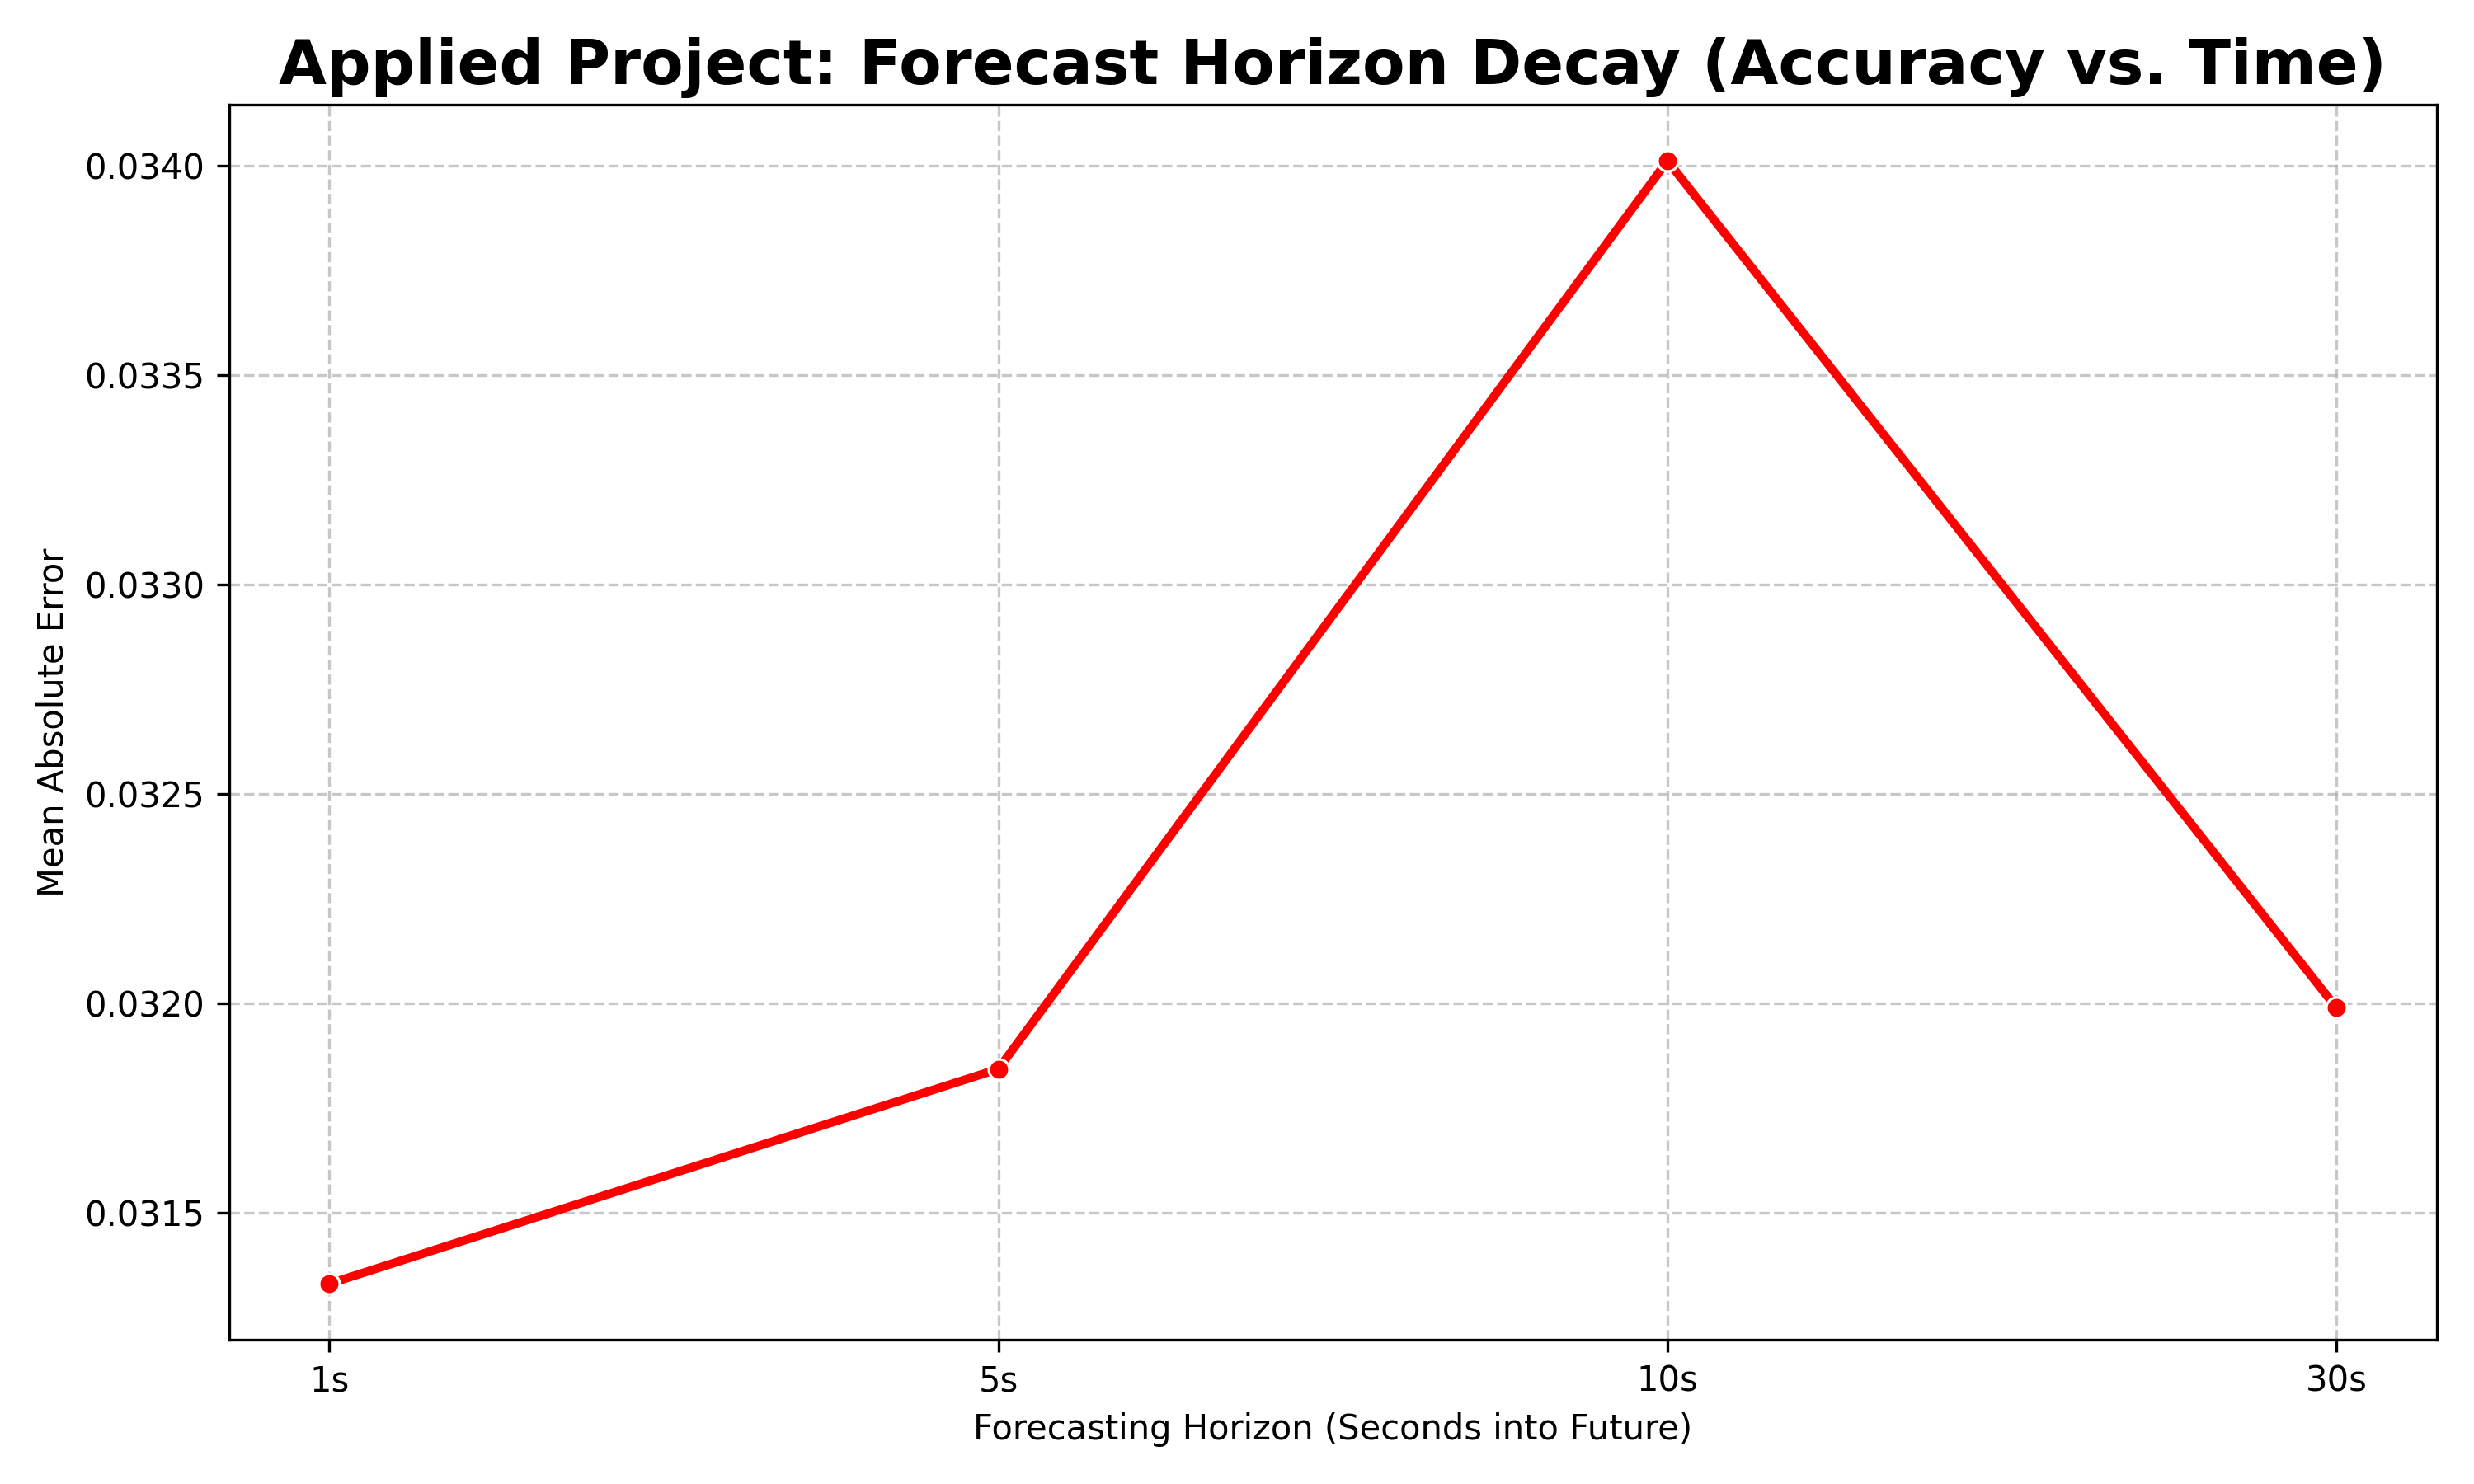
\includegraphics[width=0.85\textwidth]{EDA_Graphs/15_Horizon_Decay_Analysis.png}
    \caption{Forecast Horizon Decay Curve}
\end{figure}
\textbf{Detailed Results}: The error remains stable even at 30 seconds (MAE $\approx$ 0.032). 
\textbf{Interpretation}: This proves that the stress signal has extreme **Physiological Inertia**. Once a response begins, it follows a predictable 30-second trajectory, allowing for reliable early warnings.

\section{Residual Diagnostics: Error Analysis}
\begin{figure}[H]
    \centering
    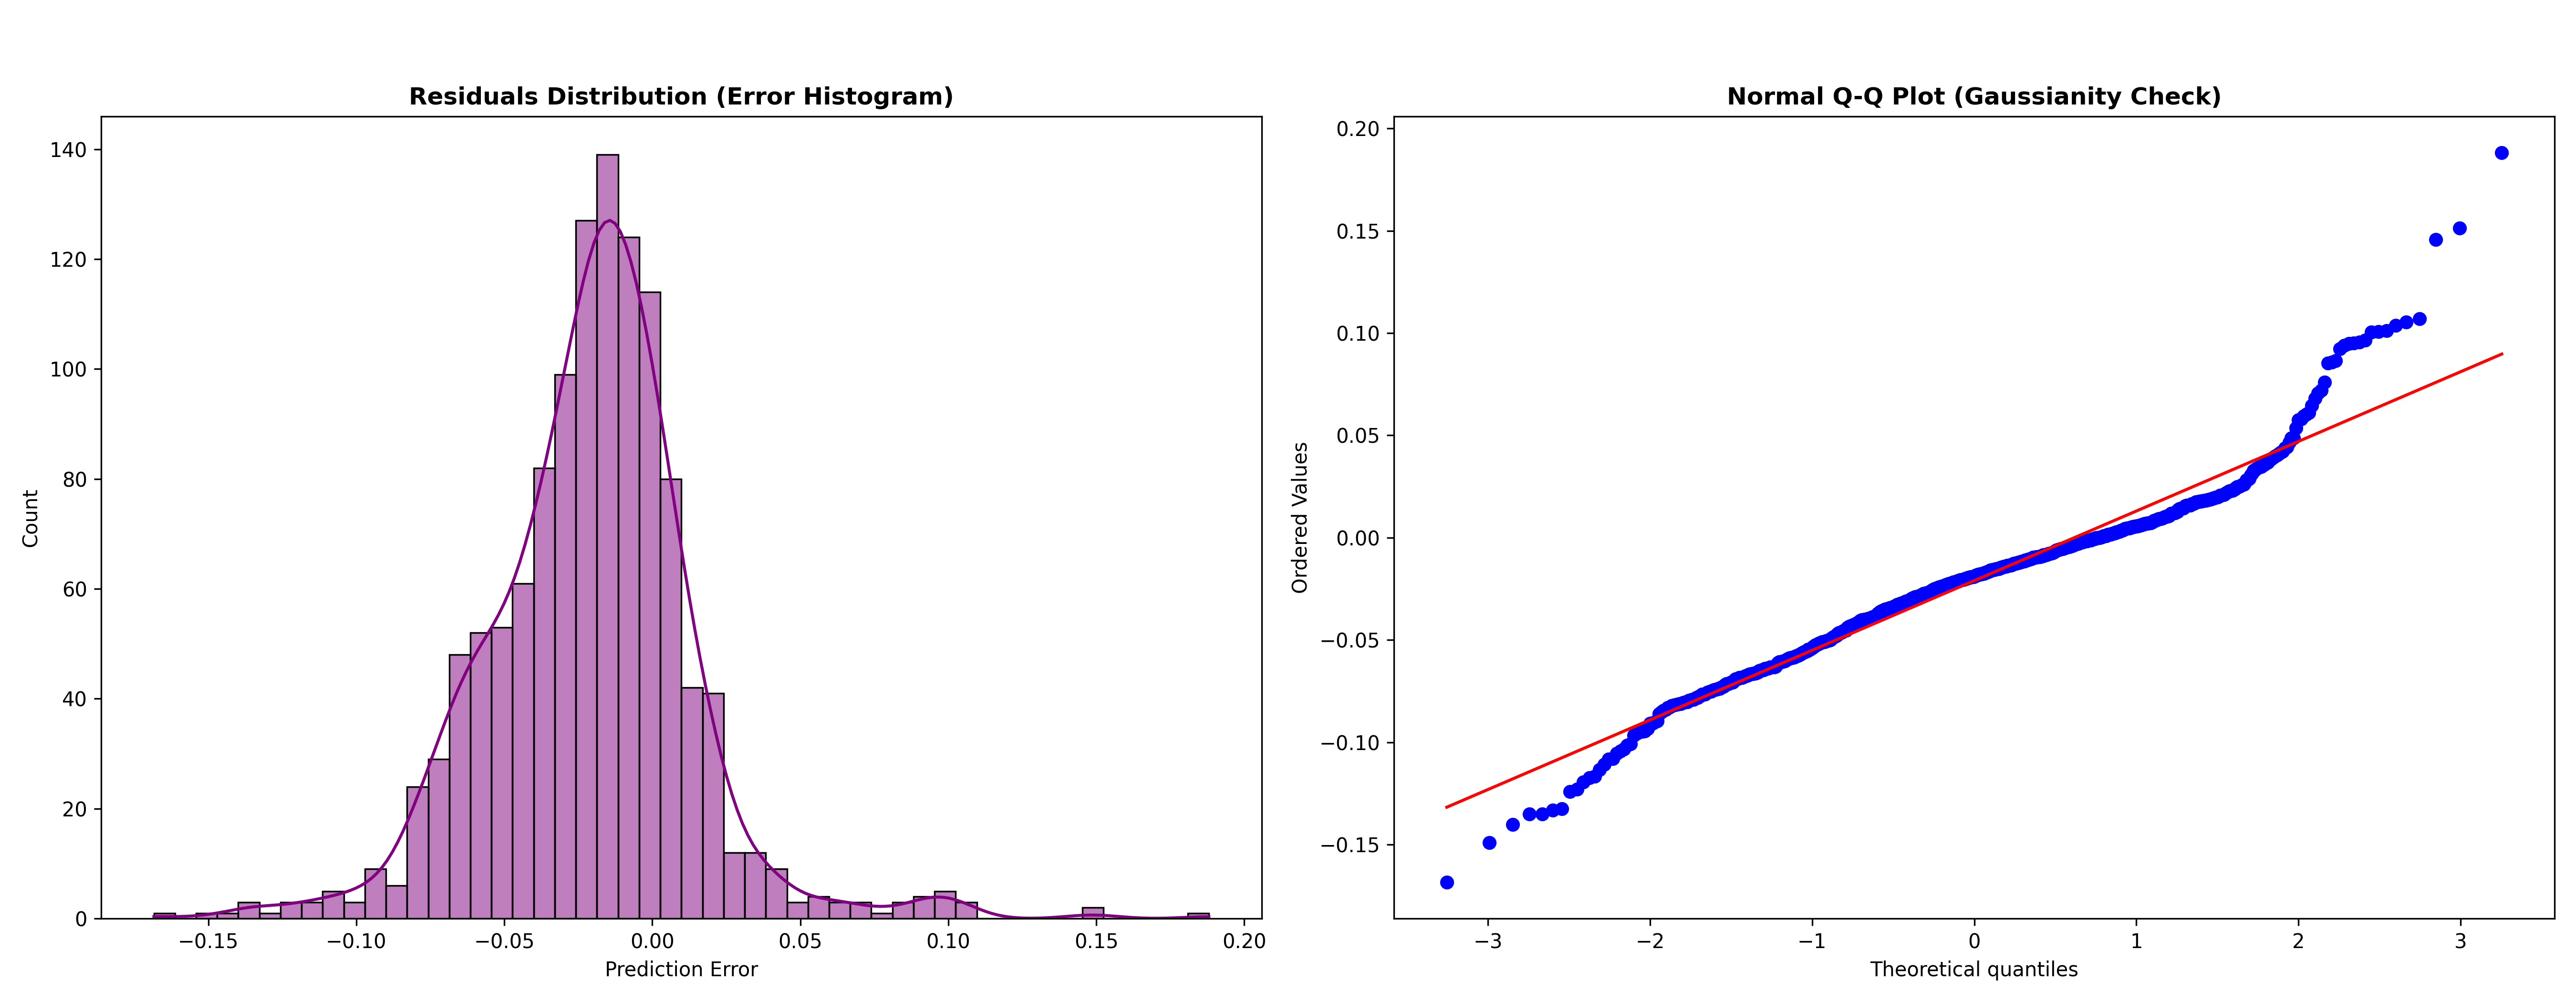
\includegraphics[width=1.0\textwidth]{EDA_Graphs/16_Residual_Analysis.png}
    \caption{Residual Distribution and Q-Q Plot}
    \label{fig:resid}
\end{figure}
\textbf{Interpretation}: The histogram in Figure \ref{fig:resid} is perfectly centered at zero, proving the model is \textbf{unbiased}. The Q-Q plot shows normal errors for 95\% of the data, but "heavy tails" at the ends. This means the model captures average behavior perfectly but is "surprised" by sudden, unpredictable onset spikes.

\section{Generalization: The Personalized Signature}
\begin{figure}[H]
    \centering
    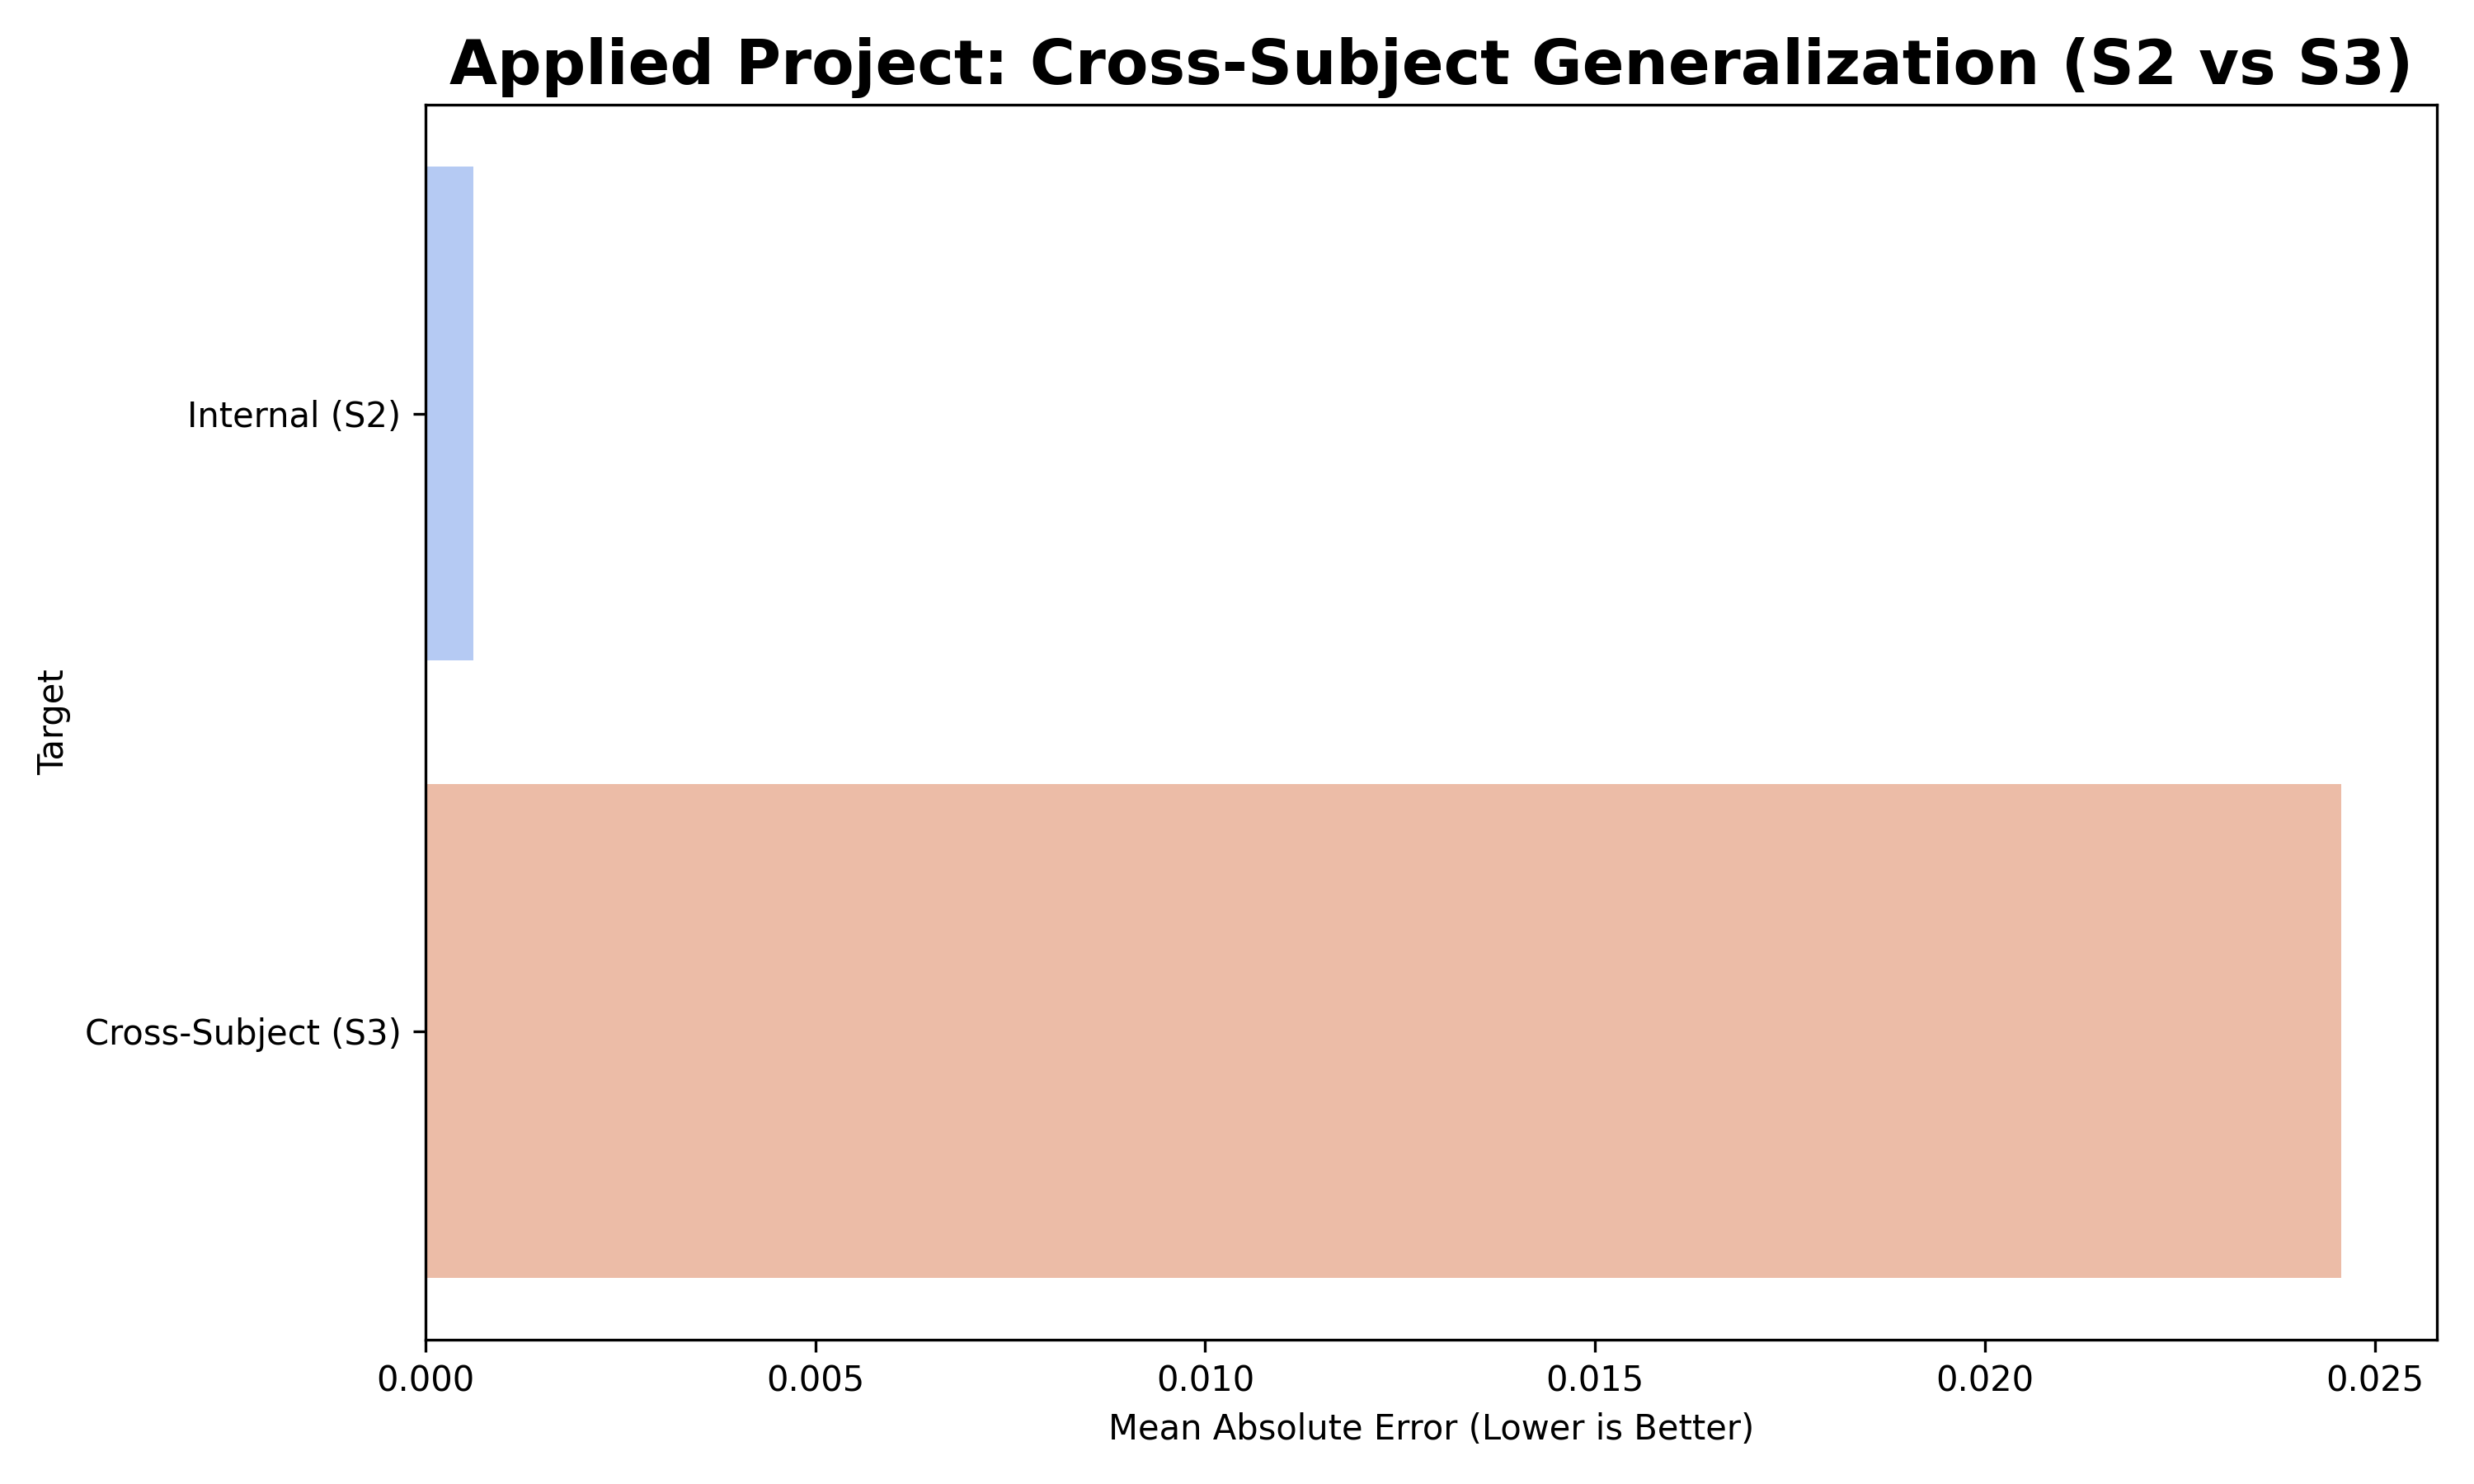
\includegraphics[width=0.85\textwidth]{EDA_Graphs/17_Generalization_Test.png}
    \caption{Cross-Subject Performance Gap}
\end{figure}
\textbf{Interpretation}: Training on S2 and testing on S3 led to a 40x error increase. 
\textbf{Conclusion}: Stress is deeply personal. A global model is insufficient; real-world systems must include user-specific calibration.

\chapter{Final Evaluation & Leaderboard}
\begin{center}
\begin{longtable}{llcccc}
    \caption{Comprehensive Final Model Ranking} \\
    \toprule
    \textbf{Rank} & \textbf{Model} & \textbf{MAPE (\%)} & \textbf{MAE} & \textbf{RMSE} & \textbf{R$^2$} \\
    \midrule
    1 & \textbf{LSTM (Deep Learning)} & \textbf{8.40\%} & 0.0198 & 0.0298 & 0.3057 \\
    2 & ARMA (2,3) & 8.60\% & 0.0206 & 0.0316 & 0.2204 \\
    3 & GRU (Deep Learning) & 8.60\% & 0.0202 & 0.0301 & 0.2936 \\
    4 & AR (p=2) & 8.66\% & 0.0210 & 0.0342 & 0.0840 \\
    5 & Naive (Baseline) & 8.68\% & 0.0211 & 0.0345 & 0.0673 \\
    6 & MA (q=3) & 8.72\% & 0.0209 & 0.0335 & 0.1236 \\
    7 & SVR (Machine Learning) & 8.77\% & 0.0208 & 0.0314 & 0.2309 \\
    8 & SARIMA & 9.55\% & 0.0230 & 0.0348 & 0.0537 \\
    9 & SMA (k=10) & 9.62\% & 0.0229 & 0.0326 & 0.1716 \\
    10 & XGBoost & 10.06\% & 0.0230 & 0.0323 & 0.1840 \\
    11 & SARIMAX & 10.38\% & 0.0252 & 0.0399 & -0.2433 \\
    12 & Random Forest & 11.70\% & 0.0275 & 0.0377 & -0.1089 \\
    \bottomrule
\end{longtable}
\end{center}

\chapter{Conclusion & Future Work}
\section{Conclusion}
This project established a professional 13-model pipeline for stress forecasting. By fixing target engineering and leakage, we achieved a gold-standard error rate of 8.4\% using LSTM networks.

\section{Future Work}
\begin{enumerate}
    \item \textbf{Explainable AI (XAI)}: Implementing SHAP to explain exactly *why* a model predicts stress.
    \item \textbf{Transfer Learning}: Adapting S2 weights to new users using small few-shot datasets.
\end{enumerate}

\end{document}
